%%____________________________________________________________________________||
\section{Results}
\label{app:results}

\subsection{Tabulated presentation of pre-fit result (signal and
  control regions)}
\label{app:results-tables-pre}

\subsubsection{Signal region}

\begin{table}[!h]
  \topcaption{
    Observed data counts and pre-fit background expectations in
    the signal region for the \texttt{eq1j} topology. The
    uncertainties in the background expectations include statistical
    contributions only. 
  }
  \label{tab:result-eq1j}
  \tiny
  \centering
  \begin{tabular}{rrllrrcl}
    \hline
    \njet\T\B & \nb & \scalht [GeV] & \mht [GeV] & Data & \multicolumn{3}{c}{SM} \\ 
    \hline
1 & 0 & $ 200- 400$ & $200-400$ & 291353 & 254856.1 &$\pm$&  424.1 \\
1 & 0 & $ 400- 600$ & $200-400$ &   8572 &   7342.2 &$\pm$&   30.1 \\
1 & 0 & $ 600- 900$ & $200-400$ &    878 &    680.1 &$\pm$&    4.0 \\
1 & 0 & $ 900- \infty$ & $200-400$ &     57 &     56.9 &$\pm$&    0.9 \\
1 & 1 & $ 200- 400$ & $200-400$ &  11072 &   8864.3 &$\pm$&   29.0 \\
1 & 1 & $ 400- 600$ & $200-400$ &    406 &    334.6 &$\pm$&    2.7 \\
1 & 1 & $ 600- \infty$ & $200-400$ &     71 &     41.5 &$\pm$&    0.5 \\
    \hline
  \end{tabular}
\end{table}

\begin{table}[!h]
  \topcaption{
    Observed data counts and pre-fit background expectations in
    the signal region for the \texttt{ge2a} topology. The
    uncertainties in the background expectations include statistical
    contributions only. 
  }
  \label{tab:result-ge2a}
  \tiny
  \centering
  \begin{tabular}{rrllrrcl}
    \hline
    \njet\T\B & \nb & \scalht [GeV] & \mht [GeV] & Data & \multicolumn{3}{c}{SM} \\ 
    \hline
$\geq 2${\it a} & 0 & $ 200- 400$ & $200-400$ & 116868 & 101411.4 &$\pm$&  392.8 \\
$\geq 2${\it a} & 0 & $ 400- 600$ & $200-400$ &   2932 &   2909.4 &$\pm$&  119.9 \\
$\geq 2${\it a} & 0 & $ 400- 600$ & $400-600$ &   2800 &   2582.2 &$\pm$&   99.5 \\
$\geq 2${\it a} & 0 & $ 600- 900$ & $200-400$ &     67 &     65.3 &$\pm$&    2.1 \\
$\geq 2${\it a} & 0 & $ 600- 900$ & $400-600$ &     73 &     63.0 &$\pm$&    1.9 \\
$\geq 2${\it a} & 0 & $ 600- 900$ & $600-900$ &    177 &    157.1 &$\pm$&    3.9 \\
$\geq 2${\it a} & 0 & $ 900- \infty$ & $200-400$ &     28 &     31.8 &$\pm$&    0.8 \\
$\geq 2${\it a} & 0 & $ 900- \infty$ & $400-600$ &     54 &     50.3 &$\pm$&    0.9 \\
$\geq 2${\it a} & 1 & $ 200- 400$ & $200-400$ &  16307 &  13333.6 &$\pm$&   57.9 \\
$\geq 2${\it a} & 1 & $ 400- 600$ & $200-400$ &   1042 &    969.1 &$\pm$&   39.6 \\
$\geq 2${\it a} & 1 & $ 400- 600$ & $400-600$ &    310 &    275.8 &$\pm$&   10.8 \\
$\geq 2${\it a} & 1 & $ 600- 900$ & $200-400$ &     12 &     18.6 &$\pm$&    0.8 \\
$\geq 2${\it a} & 1 & $ 600- 900$ & $400-600$ &     12 &     11.1 &$\pm$&    0.5 \\
$\geq 2${\it a} & 1 & $ 600- 900$ & $600-900$ &     22 &     16.9 &$\pm$&    0.5 \\
$\geq 2${\it a} & 1 & $ 900- \infty$ & $200-400$ &      5 &      3.9 &$\pm$&    0.2 \\
$\geq 2${\it a} & 1 & $ 900- \infty$ & $400-600$ &      7 &      6.3 &$\pm$&    0.2 \\
$\geq 2${\it a} & 2 & $ 200- 400$ & $200-400$ &   2200 &   1856.5 &$\pm$&   13.9 \\
$\geq 2${\it a} & 2 & $ 400- 600$ & $200-400$ &    410 &    373.9 &$\pm$&   15.4 \\
$\geq 2${\it a} & 2 & $ 400- 600$ & $400-600$ &     35 &     23.9 &$\pm$&    1.2 \\
$\geq 2${\it a} & 2 & $ 600- 900$ & $200-400$ &      5 &      6.3 &$\pm$&    0.4 \\
$\geq 2${\it a} & 2 & $ 600- 900$ & $400-600$ &      3 &      2.2 &$\pm$&    0.2 \\
$\geq 2${\it a} & 2 & $ 600- 900$ & $600-900$ &      2 &      1.4 &$\pm$&    0.1 \\
$\geq 2${\it a} & 2 & $ 900- \infty$ & $200-400$ &      1 &      0.6 &$\pm$&    0.1 \\
$\geq 2${\it a} & 2 & $ 900- \infty$ & $400-600$ &      0 &      0.4 &$\pm$&    0.0 \\
$\geq 2${\it a} & 3 & $ 200- 400$ & $200-400$ &     92 &     70.7 &$\pm$&    1.1 \\
$\geq 2${\it a} & 3 & $ 400- 600$ & $200-400$ &     38 &     34.4 &$\pm$&    1.3 \\
$\geq 2${\it a} & 3 & $ 400- 600$ & $400-600$ &      2 &      0.6 &$\pm$&    0.1 \\
$\geq 2${\it a} & 3 & $ 600- \infty$ & $200-400$ &      1 &      0.9 &$\pm$&    0.1 \\
$\geq 2${\it a} & 3 & $ 600- \infty$ & $400-600$ &      0 &      0.2 &$\pm$&    0.0 \\
$\geq 2${\it a} & 3 & $ 600- \infty$ & $600-900$ &      0 &      0.1 &$\pm$&    0.0 \\
    \hline
  \end{tabular}
\end{table}

\begin{table}[!h]
  \topcaption{
    Observed data counts and pre-fit background expectations in
    the signal region for the \texttt{eq2j} topology. The
    uncertainties in the background expectations include statistical
    contributions only. 
  }
  \label{tab:result-eq2j}
  \tiny
  \centering
  \begin{tabular}{rrllrrcl}
    \hline
    \njet\T\B & \nb & \scalht [GeV] & \mht [GeV] & Data & \multicolumn{3}{c}{SM} \\ 
    \hline
2 & 0 & $ 200- 400$ & $200-400$ &  34934 &  29224.5 &$\pm$&  147.1 \\
2 & 0 & $ 400- 600$ & $200-400$ &   3468 &   3274.3 &$\pm$&   55.0 \\
2 & 0 & $ 400- 600$ & $400-600$ &   2568 &   2176.9 &$\pm$&   35.2 \\
2 & 0 & $ 600- 900$ & $200-400$ &    226 &    276.7 &$\pm$&    5.3 \\
2 & 0 & $ 600- 900$ & $400-600$ &    253 &    268.4 &$\pm$&    5.0 \\
2 & 0 & $ 600- 900$ & $600-900$ &    303 &    284.6 &$\pm$&    5.0 \\
2 & 0 & $ 900-1200$ & $200-400$ &    165 &    179.3 &$\pm$&    3.0 \\
2 & 0 & $ 900-1200$ & $400-600$ &    125 &    130.9 &$\pm$&    2.4 \\
2 & 0 & $ 900-1200$ & $600-900$ &     97 &     78.7 &$\pm$&    1.6 \\
2 & 0 & $ 900-1200$ & $900-\infty$ &     25 &     29.3 &$\pm$&    0.8 \\
2 & 0 & $1200- \infty$ & $200-400$ &      9 &     11.8 &$\pm$&    0.6 \\
2 & 0 & $1200- \infty$ & $400-600$ &     26 &     33.4 &$\pm$&    1.2 \\
2 & 0 & $1200- \infty$ & $600-900$ &     22 &     28.0 &$\pm$&    1.0 \\
2 & 0 & $1200- \infty$ & $900-\infty$ &     19 &     20.9 &$\pm$&    0.7 \\
2 & 1 & $ 200- 400$ & $200-400$ &   3850 &   3006.6 &$\pm$&   20.8 \\
2 & 1 & $ 400- 600$ & $200-400$ &    327 &    277.4 &$\pm$&    5.3 \\
2 & 1 & $ 400- 600$ & $400-600$ &    240 &    219.3 &$\pm$&    4.2 \\
2 & 1 & $ 600- 900$ & $200-400$ &     22 &     26.9 &$\pm$&    0.6 \\
2 & 1 & $ 600- 900$ & $400-600$ &     39 &     25.5 &$\pm$&    0.7 \\
2 & 1 & $ 600- 900$ & $600-900$ &     31 &     27.1 &$\pm$&    0.7 \\
2 & 1 & $ 900-1200$ & $200-400$ &     17 &     19.3 &$\pm$&    0.4 \\
2 & 1 & $ 900-1200$ & $400-600$ &     15 &     14.9 &$\pm$&    0.4 \\
2 & 1 & $ 900-1200$ & $600-900$ &     12 &      7.4 &$\pm$&    0.2 \\
2 & 1 & $ 900-1200$ & $900-\infty$ &      6 &      3.2 &$\pm$&    0.1 \\
2 & 1 & $1200- \infty$ & $200-400$ &      1 &      1.1 &$\pm$&    0.1 \\
2 & 1 & $1200- \infty$ & $400-600$ &      6 &      3.4 &$\pm$&    0.1 \\
2 & 1 & $1200- \infty$ & $600-900$ &      1 &      2.1 &$\pm$&    0.1 \\
2 & 1 & $1200- \infty$ & $900-\infty$ &      4 &      2.0 &$\pm$&    0.1 \\
2 & 2 & $ 200- 400$ & $200-400$ &    254 &    196.1 &$\pm$&    4.4 \\
2 & 2 & $ 400- 600$ & $200-400$ &     22 &     13.2 &$\pm$&    0.5 \\
2 & 2 & $ 400- 600$ & $400-600$ &     18 &     15.2 &$\pm$&    0.6 \\
2 & 2 & $ 600- \infty$ & $200-400$ &      1 &      1.8 &$\pm$&    0.1 \\
2 & 2 & $ 600- \infty$ & $400-600$ &      2 &      1.9 &$\pm$&    0.1 \\
2 & 2 & $ 600- \infty$ & $600-900$ &      2 &      2.3 &$\pm$&    0.1 \\
    \hline
  \end{tabular}
\end{table}

\begin{table}[!h]
  \topcaption{
    Observed data counts and pre-fit background expectations in
    the signal region for the \texttt{eq3j} topology. The
    uncertainties in the background expectations include statistical
    contributions only. 
  }
  \label{tab:result-eq3j}
  \tiny
  \centering
  \begin{tabular}{rrllrrcl}
    \hline
    \njet\T\B & \nb & \scalht [GeV] & \mht [GeV] & Data & \multicolumn{3}{c}{SM} \\ 
    \hline
3 & 0 & $ 200- 400$ & $200-400$ &  11815 &  10504.3 &$\pm$&   82.8 \\
3 & 0 & $ 400- 600$ & $200-400$ &   7120 &   6666.9 &$\pm$&   34.0 \\
3 & 0 & $ 400- 600$ & $400-600$ &   1463 &   1391.0 &$\pm$&   11.6 \\
3 & 0 & $ 600- 900$ & $200-400$ &    668 &    698.5 &$\pm$&   24.7 \\
3 & 0 & $ 600- 900$ & $400-600$ &    593 &    582.0 &$\pm$&   20.3 \\
3 & 0 & $ 600- 900$ & $600-900$ &    246 &    231.4 &$\pm$&    7.9 \\
3 & 0 & $ 900-1200$ & $200-400$ &    245 &    275.3 &$\pm$&    3.3 \\
3 & 0 & $ 900-1200$ & $400-600$ &    164 &    182.3 &$\pm$&    2.4 \\
3 & 0 & $ 900-1200$ & $600-900$ &    101 &    109.8 &$\pm$&    1.7 \\
3 & 0 & $ 900-1200$ & $900-\infty$ &     19 &     28.2 &$\pm$&    0.8 \\
3 & 0 & $1200- \infty$ & $200-400$ &     21 &     22.5 &$\pm$&    0.8 \\
3 & 0 & $1200- \infty$ & $400-600$ &     28 &     54.2 &$\pm$&    1.4 \\
3 & 0 & $1200- \infty$ & $600-900$ &     31 &     36.1 &$\pm$&    0.9 \\
3 & 0 & $1200- \infty$ & $900-\infty$ &     17 &     22.0 &$\pm$&    0.6 \\
3 & 1 & $ 200- 400$ & $200-400$ &   2703 &   2242.6 &$\pm$&   19.1 \\
3 & 1 & $ 400- 600$ & $200-400$ &   1212 &   1125.8 &$\pm$&    7.7 \\
3 & 1 & $ 400- 600$ & $400-600$ &    301 &    222.4 &$\pm$&    3.1 \\
3 & 1 & $ 600- 900$ & $200-400$ &    110 &     94.6 &$\pm$&    3.4 \\
3 & 1 & $ 600- 900$ & $400-600$ &     96 &     77.9 &$\pm$&    2.8 \\
3 & 1 & $ 600- 900$ & $600-900$ &     42 &     32.7 &$\pm$&    1.2 \\
3 & 1 & $ 900-1200$ & $200-400$ &     39 &     41.2 &$\pm$&    0.7 \\
3 & 1 & $ 900-1200$ & $400-600$ &     24 &     23.9 &$\pm$&    0.4 \\
3 & 1 & $ 900-1200$ & $600-900$ &     10 &     15.4 &$\pm$&    0.3 \\
3 & 1 & $ 900-1200$ & $900-\infty$ &      6 &      4.4 &$\pm$&    0.3 \\
3 & 1 & $1200- \infty$ & $200-400$ &      3 &      3.4 &$\pm$&    0.1 \\
3 & 1 & $1200- \infty$ & $400-600$ &      5 &      7.5 &$\pm$&    0.2 \\
3 & 1 & $1200- \infty$ & $600-900$ &      7 &      5.1 &$\pm$&    0.2 \\
3 & 1 & $1200- \infty$ & $900-\infty$ &      4 &      3.5 &$\pm$&    0.1 \\
3 & 2 & $ 200- 400$ & $200-400$ &    495 &    418.2 &$\pm$&    5.7 \\
3 & 2 & $ 400- 600$ & $200-400$ &    229 &    208.3 &$\pm$&    3.0 \\
3 & 2 & $ 400- 600$ & $400-600$ &     34 &     27.0 &$\pm$&    0.8 \\
3 & 2 & $ 600- 900$ & $200-400$ &     10 &      9.1 &$\pm$&    0.4 \\
3 & 2 & $ 600- 900$ & $400-600$ &      9 &      9.3 &$\pm$&    0.5 \\
3 & 2 & $ 600- 900$ & $600-900$ &      2 &      3.2 &$\pm$&    0.1 \\
3 & 2 & $ 900-1200$ & $200-400$ &      4 &      3.5 &$\pm$&    0.2 \\
3 & 2 & $ 900-1200$ & $400-600$ &      2 &      1.8 &$\pm$&    0.1 \\
3 & 2 & $ 900-1200$ & $600-900$ &      2 &      1.3 &$\pm$&    0.1 \\
3 & 2 & $ 900-1200$ & $900-\infty$ &      0 &      0.4 &$\pm$&    0.1 \\
3 & 2 & $1200- \infty$ & $200-400$ &      1 &      0.3 &$\pm$&    0.0 \\
3 & 2 & $1200- \infty$ & $400-600$ &      0 &      0.7 &$\pm$&    0.0 \\
3 & 2 & $1200- \infty$ & $600-900$ &      0 &      0.4 &$\pm$&    0.0 \\
3 & 2 & $1200- \infty$ & $900-\infty$ &      0 &      0.3 &$\pm$&    0.0 \\
3 & 3 & $ 200- 400$ & $200-400$ &     16 &     12.1 &$\pm$&    0.3 \\
3 & 3 & $ 400- 600$ & $200-400$ &     10 &      7.9 &$\pm$&    0.2 \\
3 & 3 & $ 400- 600$ & $400-600$ &      2 &      0.8 &$\pm$&    0.1 \\
3 & 3 & $ 600- \infty$ & $200-400$ &      3 &      0.4 &$\pm$&    0.0 \\
3 & 3 & $ 600- \infty$ & $400-600$ &      3 &      0.3 &$\pm$&    0.0 \\
3 & 3 & $ 600- \infty$ & $600-900$ &      0 &      0.2 &$\pm$&    0.0 \\
    \hline
  \end{tabular}
\end{table}

\begin{table}[!h]
  \topcaption{
    Observed data counts and pre-fit background expectations in
    the signal region for the \texttt{eq4j} topology. The
    uncertainties in the background expectations include statistical
    contributions only. 
  }
  \label{tab:result-eq4j}
  \tiny
  \centering
  \begin{tabular}{rrllrrcl}
    \hline
    \njet\T\B & \nb & \scalht [GeV] & \mht [GeV] & Data & \multicolumn{3}{c}{SM} \\ 
    \hline
4 & 0 & $ 400- 600$ & $200-400$ &   4324 &   4749.1 &$\pm$&   27.6 \\
4 & 0 & $ 400- 600$ & $400-600$ &    437 &    460.4 &$\pm$&    6.4 \\
4 & 0 & $ 600- 900$ & $200-400$ &    751 &    937.0 &$\pm$&    6.6 \\
4 & 0 & $ 600- 900$ & $400-600$ &    484 &    521.7 &$\pm$&    4.5 \\
4 & 0 & $ 600- 900$ & $600-900$ &    110 &    103.7 &$\pm$&    1.6 \\
4 & 0 & $ 900-1200$ & $200-400$ &    186 &    251.2 &$\pm$&    3.2 \\
4 & 0 & $ 900-1200$ & $400-600$ &    111 &    142.9 &$\pm$&    2.2 \\
4 & 0 & $ 900-1200$ & $600-900$ &     66 &     71.7 &$\pm$&    1.3 \\
4 & 0 & $ 900-1200$ & $900-\infty$ &     13 &     10.6 &$\pm$&    0.5 \\
4 & 0 & $1200- \infty$ & $200-400$ &     13 &     23.8 &$\pm$&    0.7 \\
4 & 0 & $1200- \infty$ & $400-600$ &     32 &     43.0 &$\pm$&    1.0 \\
4 & 0 & $1200- \infty$ & $600-900$ &     28 &     26.8 &$\pm$&    0.6 \\
4 & 0 & $1200- \infty$ & $900-\infty$ &     15 &     13.9 &$\pm$&    0.3 \\
4 & 1 & $ 400- 600$ & $200-400$ &   1497 &   1444.4 &$\pm$&    9.2 \\
4 & 1 & $ 400- 600$ & $400-600$ &    109 &    109.8 &$\pm$&    2.2 \\
4 & 1 & $ 600- 900$ & $200-400$ &    184 &    196.6 &$\pm$&    2.1 \\
4 & 1 & $ 600- 900$ & $400-600$ &    106 &    100.9 &$\pm$&    1.3 \\
4 & 1 & $ 600- 900$ & $600-900$ &     19 &     17.2 &$\pm$&    0.4 \\
4 & 1 & $ 900-1200$ & $200-400$ &     60 &     53.8 &$\pm$&    0.8 \\
4 & 1 & $ 900-1200$ & $400-600$ &     19 &     27.7 &$\pm$&    0.5 \\
4 & 1 & $ 900-1200$ & $600-900$ &     11 &     12.3 &$\pm$&    0.3 \\
4 & 1 & $ 900-1200$ & $900-\infty$ &      1 &      1.8 &$\pm$&    0.1 \\
4 & 1 & $1200- \infty$ & $200-400$ &      7 &      5.2 &$\pm$&    0.2 \\
4 & 1 & $1200- \infty$ & $400-600$ &     11 &     10.6 &$\pm$&    0.2 \\
4 & 1 & $1200- \infty$ & $600-900$ &      7 &      4.8 &$\pm$&    0.1 \\
4 & 1 & $1200- \infty$ & $900-\infty$ &      4 &      2.9 &$\pm$&    0.1 \\
4 & 2 & $ 400- 600$ & $200-400$ &    524 &    490.0 &$\pm$&    5.0 \\
4 & 2 & $ 400- 600$ & $400-600$ &     29 &     24.0 &$\pm$&    0.9 \\
4 & 2 & $ 600- 900$ & $200-400$ &     50 &     39.2 &$\pm$&    0.9 \\
4 & 2 & $ 600- 900$ & $400-600$ &     19 &     19.9 &$\pm$&    0.6 \\
4 & 2 & $ 600- 900$ & $600-900$ &      1 &      2.4 &$\pm$&    0.1 \\
4 & 2 & $ 900-1200$ & $200-400$ &     10 &      8.7 &$\pm$&    0.3 \\
4 & 2 & $ 900-1200$ & $400-600$ &      7 &      4.1 &$\pm$&    0.2 \\
4 & 2 & $ 900-1200$ & $600-900$ &      0 &      1.7 &$\pm$&    0.1 \\
4 & 2 & $ 900-1200$ & $900-\infty$ &      1 &      0.3 &$\pm$&    0.0 \\
4 & 2 & $1200- \infty$ & $200-400$ &      1 &      0.7 &$\pm$&    0.1 \\
4 & 2 & $1200- \infty$ & $400-600$ &      0 &      1.5 &$\pm$&    0.1 \\
4 & 2 & $1200- \infty$ & $600-900$ &      0 &      0.5 &$\pm$&    0.0 \\
4 & 2 & $1200- \infty$ & $900-\infty$ &      1 &      0.4 &$\pm$&    0.0 \\
4 & 3 & $ 400- 600$ & $200-400$ &     35 &     36.8 &$\pm$&    0.6 \\
4 & 3 & $ 400- 600$ & $400-600$ &      1 &      1.6 &$\pm$&    0.1 \\
4 & 3 & $ 600- 900$ & $200-400$ &      6 &      2.5 &$\pm$&    0.1 \\
4 & 3 & $ 600- 900$ & $400-600$ &      0 &      1.2 &$\pm$&    0.1 \\
4 & 3 & $ 600- 900$ & $600-900$ &      0 &      0.2 &$\pm$&    0.0 \\
4 & 3 & $ 900- \infty$ & $200-400$ &      0 &      0.7 &$\pm$&    0.0 \\
4 & 3 & $ 900- \infty$ & $400-600$ &      0 &      0.4 &$\pm$&    0.0 \\
4 & 3 & $ 900- \infty$ & $600-900$ &      0 &      0.1 &$\pm$&    0.0 \\
4 & 3 & $ 900- \infty$ & $900-\infty$ &      0 &      0.0 &$\pm$&    0.0 \\
    \hline
  \end{tabular}
\end{table}

\begin{table}[!h]
  \topcaption{
    Observed data counts and pre-fit background expectations in
    the signal region for the \texttt{eq5j} topology. The
    uncertainties in the background expectations include statistical
    contributions only. 
  }
  \label{tab:result-eq5j}
  \tiny
  \centering
  \begin{tabular}{rrllrrcl}
    \hline
    \njet\T\B & \nb & \scalht [GeV] & \mht [GeV] & Data & \multicolumn{3}{c}{SM} \\ 
    \hline
5 & 0 & $ 400- 600$ & $200-400$ &   1132 &   1250.0 &$\pm$&  164.1 \\
5 & 0 & $ 400- 600$ & $400-600$ &     59 &     74.0 &$\pm$&   10.6 \\
5 & 0 & $ 600- 900$ & $200-400$ &    435 &    561.4 &$\pm$&   19.4 \\
5 & 0 & $ 600- 900$ & $400-600$ &    201 &    197.5 &$\pm$&    6.8 \\
5 & 0 & $ 600- 900$ & $600-900$ &     17 &     25.9 &$\pm$&    1.1 \\
5 & 0 & $ 900-1200$ & $200-400$ &    124 &    149.9 &$\pm$&    2.4 \\
5 & 0 & $ 900-1200$ & $400-600$ &     59 &     68.1 &$\pm$&    1.5 \\
5 & 0 & $ 900-1200$ & $600-900$ &     28 &     30.7 &$\pm$&    0.8 \\
5 & 0 & $1200- \infty$ & $200-400$ &      7 &     18.1 &$\pm$&    0.6 \\
5 & 0 & $1200- \infty$ & $400-600$ &     16 &     23.1 &$\pm$&    0.7 \\
5 & 0 & $1200- \infty$ & $600-900$ &      7 &     13.2 &$\pm$&    0.4 \\
5 & 0 & $1200- \infty$ & $900-\infty$ &      6 &      6.2 &$\pm$&    0.2 \\
5 & 1 & $ 400- 600$ & $200-400$ &    591 &    608.6 &$\pm$&   79.9 \\
5 & 1 & $ 400- 600$ & $400-600$ &     22 &     22.0 &$\pm$&    3.3 \\
5 & 1 & $ 600- 900$ & $200-400$ &    198 &    194.1 &$\pm$&    7.1 \\
5 & 1 & $ 600- 900$ & $400-600$ &     50 &     55.2 &$\pm$&    2.1 \\
5 & 1 & $ 600- 900$ & $600-900$ &     11 &      5.9 &$\pm$&    0.3 \\
5 & 1 & $ 900-1200$ & $200-400$ &     33 &     41.0 &$\pm$&    0.7 \\
5 & 1 & $ 900-1200$ & $400-600$ &     15 &     16.9 &$\pm$&    0.4 \\
5 & 1 & $ 900-1200$ & $600-900$ &      9 &      6.9 &$\pm$&    0.2 \\
5 & 1 & $1200- \infty$ & $200-400$ &      4 &      4.5 &$\pm$&    0.1 \\
5 & 1 & $1200- \infty$ & $400-600$ &      3 &      6.1 &$\pm$&    0.2 \\
5 & 1 & $1200- \infty$ & $600-900$ &      5 &      2.8 &$\pm$&    0.1 \\
5 & 1 & $1200- \infty$ & $900-\infty$ &      2 &      1.6 &$\pm$&    0.1 \\
5 & 2 & $ 400- 600$ & $200-400$ &    284 &    273.9 &$\pm$&   36.1 \\
5 & 2 & $ 400- 600$ & $400-600$ &     10 &      4.8 &$\pm$&    0.7 \\
5 & 2 & $ 600- 900$ & $200-400$ &     63 &     67.5 &$\pm$&    2.7 \\
5 & 2 & $ 600- 900$ & $400-600$ &     16 &     16.5 &$\pm$&    0.8 \\
5 & 2 & $ 600- 900$ & $600-900$ &      0 &      1.3 &$\pm$&    0.1 \\
5 & 2 & $ 900-1200$ & $200-400$ &      5 &     10.5 &$\pm$&    0.3 \\
5 & 2 & $ 900-1200$ & $400-600$ &      5 &      3.5 &$\pm$&    0.2 \\
5 & 2 & $ 900-1200$ & $600-900$ &      1 &      1.5 &$\pm$&    0.1 \\
5 & 2 & $1200- \infty$ & $200-400$ &      0 &      1.0 &$\pm$&    0.1 \\
5 & 2 & $1200- \infty$ & $400-600$ &      2 &      1.2 &$\pm$&    0.1 \\
5 & 2 & $1200- \infty$ & $600-900$ &      1 &      0.4 &$\pm$&    0.0 \\
5 & 2 & $1200- \infty$ & $900-\infty$ &      1 &      0.3 &$\pm$&    0.0 \\
5 & 3 & $ 400- 600$ & $200-400$ &     25 &     28.0 &$\pm$&    3.7 \\
5 & 3 & $ 400- 600$ & $400-600$ &      1 &      0.3 &$\pm$&    0.1 \\
5 & 3 & $ 600- 900$ & $200-400$ &      7 &      7.5 &$\pm$&    0.4 \\
5 & 3 & $ 600- 900$ & $400-600$ &      3 &      1.5 &$\pm$&    0.1 \\
5 & 3 & $ 600- 900$ & $600-900$ &      0 &      0.1 &$\pm$&    0.0 \\
5 & 3 & $ 900- \infty$ & $200-400$ &      0 &      1.1 &$\pm$&    0.0 \\
5 & 3 & $ 900- \infty$ & $400-600$ &      0 &      0.4 &$\pm$&    0.0 \\
5 & 3 & $ 900- \infty$ & $600-900$ &      0 &      0.2 &$\pm$&    0.0 \\
5 & $\geq 4$ & $ 400- \infty$ & $200-400$ &      2 &      1.8 &$\pm$&    0.3 \\
5 & $\geq 4$ & $ 400- \infty$ & $400-600$ &      1 &      0.1 &$\pm$&    0.0 \\
    \hline
  \end{tabular}
\end{table}

\begin{table}[!h]
  \topcaption{
    Observed data counts and pre-fit background expectations in
    the signal region for the \texttt{ge6j} topology. The
    uncertainties in the background expectations include statistical
    contributions only. 
  }
  \label{tab:result-ge6j}
  \tiny
  \centering
  \begin{tabular}{rrllrrcl}
    \hline
    \njet\T\B & \nb & \scalht [GeV] & \mht [GeV] & Data & \multicolumn{3}{c}{SM} \\ 
    \hline
$\geq 6$ & 0 & $ 400- 600$ & $200-400$ &    164 &    193.7 &$\pm$&  358.5 \\
$\geq 6$ & 0 & $ 600- 900$ & $200-400$ &    210 &    278.0 &$\pm$&   13.0 \\
$\geq 6$ & 0 & $ 600- 900$ & $400-600$ &     56 &     68.1 &$\pm$&    3.3 \\
$\geq 6$ & 0 & $ 900-1200$ & $200-400$ &     64 &     94.4 &$\pm$&    1.7 \\
$\geq 6$ & 0 & $ 900-1200$ & $400-600$ &     35 &     40.1 &$\pm$&    1.1 \\
$\geq 6$ & 0 & $ 900-1200$ & $600-900$ &      6 &      6.1 &$\pm$&    0.3 \\
$\geq 6$ & 0 & $1200- \infty$ & $200-400$ &     12 &     18.3 &$\pm$&    0.5 \\
$\geq 6$ & 0 & $1200- \infty$ & $400-600$ &      9 &     16.8 &$\pm$&    0.5 \\
$\geq 6$ & 0 & $1200- \infty$ & $600-900$ &     11 &      8.6 &$\pm$&    0.3 \\
$\geq 6$ & 0 & $1200- \infty$ & $900-\infty$ &      5 &      2.8 &$\pm$&    0.1 \\
$\geq 6$ & 1 & $ 400- 600$ & $200-400$ &    121 &    135.4 &$\pm$&  249.5 \\
$\geq 6$ & 1 & $ 600- 900$ & $200-400$ &    148 &    154.3 &$\pm$&    7.5 \\
$\geq 6$ & 1 & $ 600- 900$ & $400-600$ &     26 &     25.4 &$\pm$&    1.4 \\
$\geq 6$ & 1 & $ 900-1200$ & $200-400$ &     42 &     41.7 &$\pm$&    0.6 \\
$\geq 6$ & 1 & $ 900-1200$ & $400-600$ &     12 &     13.8 &$\pm$&    0.4 \\
$\geq 6$ & 1 & $ 900-1200$ & $600-900$ &      0 &      1.7 &$\pm$&    0.1 \\
$\geq 6$ & 1 & $1200- \infty$ & $200-400$ &      6 &      7.4 &$\pm$&    0.2 \\
$\geq 6$ & 1 & $1200- \infty$ & $400-600$ &      5 &      5.9 &$\pm$&    0.2 \\
$\geq 6$ & 1 & $1200- \infty$ & $600-900$ &      5 &      2.6 &$\pm$&    0.1 \\
$\geq 6$ & 1 & $1200- \infty$ & $900-\infty$ &      0 &      0.8 &$\pm$&    0.0 \\
$\geq 6$ & 2 & $ 400- 600$ & $200-400$ &     58 &     69.5 &$\pm$&  129.2 \\
$\geq 6$ & 2 & $ 600- 900$ & $200-400$ &     85 &     74.4 &$\pm$&    3.7 \\
$\geq 6$ & 2 & $ 600- 900$ & $400-600$ &      8 &      8.5 &$\pm$&    0.6 \\
$\geq 6$ & 2 & $ 900-1200$ & $200-400$ &     11 &     17.9 &$\pm$&    0.4 \\
$\geq 6$ & 2 & $ 900-1200$ & $400-600$ &      3 &      4.6 &$\pm$&    0.2 \\
$\geq 6$ & 2 & $ 900-1200$ & $600-900$ &      0 &      0.5 &$\pm$&    0.1 \\
$\geq 6$ & 2 & $1200- \infty$ & $200-400$ &      0 &      2.5 &$\pm$&    0.1 \\
$\geq 6$ & 2 & $1200- \infty$ & $400-600$ &      0 &      1.6 &$\pm$&    0.1 \\
$\geq 6$ & 2 & $1200- \infty$ & $600-900$ &      2 &      0.6 &$\pm$&    0.0 \\
$\geq 6$ & 2 & $1200- \infty$ & $900-\infty$ &      0 &      0.2 &$\pm$&    0.0 \\
$\geq 6$ & 3 & $ 400- 600$ & $200-400$ &     14 &      8.9 &$\pm$&   17.0 \\
$\geq 6$ & 3 & $ 600- 900$ & $200-400$ &     20 &     11.1 &$\pm$&    0.6 \\
$\geq 6$ & 3 & $ 600- 900$ & $400-600$ &      3 &      1.1 &$\pm$&    0.1 \\
$\geq 6$ & 3 & $ 900-1200$ & $200-400$ &      4 &      3.0 &$\pm$&    0.1 \\
$\geq 6$ & 3 & $ 900-1200$ & $400-600$ &      0 &      0.7 &$\pm$&    0.1 \\
$\geq 6$ & 3 & $ 900-1200$ & $600-900$ &      0 &      0.1 &$\pm$&    0.0 \\
$\geq 6$ & 3 & $1200- \infty$ & $200-400$ &      1 &      0.4 &$\pm$&    0.0 \\
$\geq 6$ & 3 & $1200- \infty$ & $400-600$ &      0 &      0.2 &$\pm$&    0.0 \\
$\geq 6$ & 3 & $1200- \infty$ & $600-900$ &      1 &      0.1 &$\pm$&    0.0 \\
$\geq 6$ & 3 & $1200- \infty$ & $900-\infty$ &      0 &      0.0 &$\pm$&    0.0 \\
$\geq 6$ & $\geq 4$ & $ 400- 600$ & $200-400$ &      4 &      2.5 &$\pm$&    5.0 \\
    \hline
  \end{tabular}
\end{table}

\clearpage 
\subsubsection{Control regions}

\begin{table}[!h]
  \topcaption{
    Observed data counts and pre-fit background expectations in
    the \mj and \mmj control regions for the \texttt{eq1j} topology. The
    uncertainties in the background expectations include statistical
    contributions only. 
  }
  \label{tab:result-eq1j}
  \tiny
  \centering
  \begin{tabular}{lrrlrrcl}
    \hline
    Region\T\B & \njet & \nb & \scalht [GeV] & Data & \multicolumn{3}{c}{SM} \\ 
    \hline
    \hline
  \end{tabular}
\end{table}

\begin{table}[!h]
  \topcaption{
    Observed data counts and pre-fit background expectations in
    the \mj and \mmj control regions for the \texttt{ge2a} topology. The
    uncertainties in the background expectations include statistical
    contributions only. 
  }
  \label{tab:result-ge2a}
  \tiny
  \centering
  \begin{tabular}{lrrlrrcl}
    \hline
    Region\T\B & \njet & \nb & \scalht [GeV] & Data & \multicolumn{3}{c}{SM} \\ 
    \hline
\mj & $\geq 2${\it a} & 0 & $ 200- 250$ &  23634 &  22226.2 &$\pm$&   80.5 \\
\mj & $\geq 2${\it a} & 0 & $ 250- 300$ &  22465 &  20617.4 &$\pm$&   78.4 \\
\mj & $\geq 2${\it a} & 0 & $ 300- 350$ &  16561 &  15550.5 &$\pm$&   66.9 \\
\mj & $\geq 2${\it a} & 0 & $ 350- 400$ &  10147 &   9903.9 &$\pm$&   51.7 \\
\mj & $\geq 2${\it a} & 0 & $ 400- 500$ &   8813 &   8590.1 &$\pm$&   41.8 \\
\mj & $\geq 2${\it a} & 0 & $ 500- 600$ &   2527 &   2512.7 &$\pm$&   13.8 \\
\mj & $\geq 2${\it a} & 0 & $ 600- 750$ &   1000 &    912.5 &$\pm$&    4.5 \\
\mj & $\geq 2${\it a} & 0 & $ 750- 900$ &    214 &    185.4 &$\pm$&    1.8 \\
\mj & $\geq 2${\it a} & 0 & $ 900- \infty$ &     71 &     71.4 &$\pm$&    0.9 \\
\mj & $\geq 2${\it a} & 1 & $ 200- 250$ &   4399 &   3668.5 &$\pm$&   13.9 \\
\mj & $\geq 2${\it a} & 1 & $ 250- 300$ &   5272 &   4537.7 &$\pm$&   14.9 \\
\mj & $\geq 2${\it a} & 1 & $ 300- 350$ &   4386 &   3758.3 &$\pm$&   14.3 \\
\mj & $\geq 2${\it a} & 1 & $ 350- 400$ &   3098 &   2776.5 &$\pm$&   12.2 \\
\mj & $\geq 2${\it a} & 1 & $ 400- 500$ &   3038 &   2596.0 &$\pm$&   11.2 \\
\mj & $\geq 2${\it a} & 1 & $ 500- 600$ &    912 &    791.6 &$\pm$&    5.4 \\
\mj & $\geq 2${\it a} & 1 & $ 600- 750$ &    337 &    290.2 &$\pm$&    2.8 \\
\mj & $\geq 2${\it a} & 1 & $ 750- 900$ &     78 &     56.2 &$\pm$&    0.7 \\
\mj & $\geq 2${\it a} & 1 & $ 900- \infty$ &     17 &     16.7 &$\pm$&    0.3 \\
\mj & $\geq 2${\it a} & 2 & $ 200- 250$ &    281 &    263.7 &$\pm$&    3.1 \\
\mj & $\geq 2${\it a} & 2 & $ 250- 300$ &    685 &    589.8 &$\pm$&    4.2 \\
\mj & $\geq 2${\it a} & 2 & $ 300- 350$ &    971 &    882.9 &$\pm$&    5.7 \\
\mj & $\geq 2${\it a} & 2 & $ 350- 400$ &    952 &    869.3 &$\pm$&    5.5 \\
\mj & $\geq 2${\it a} & 2 & $ 400- 500$ &    982 &    941.9 &$\pm$&    5.8 \\
\mj & $\geq 2${\it a} & 2 & $ 500- 600$ &    331 &    287.3 &$\pm$&    2.8 \\
\mj & $\geq 2${\it a} & 2 & $ 600- 750$ &    104 &    109.7 &$\pm$&    1.6 \\
\mj & $\geq 2${\it a} & 2 & $ 750- 900$ &     23 &     19.3 &$\pm$&    0.4 \\
\mj & $\geq 2${\it a} & 2 & $ 900- \infty$ &     10 &      4.7 &$\pm$&    0.2 \\
\mj & $\geq 2${\it a} & 3 & $ 200- 250$ &      2 &      2.9 &$\pm$&    0.2 \\
\mj & $\geq 2${\it a} & 3 & $ 250- 300$ &     11 &     17.7 &$\pm$&    0.3 \\
\mj & $\geq 2${\it a} & 3 & $ 300- 350$ &     48 &     43.9 &$\pm$&    0.5 \\
\mj & $\geq 2${\it a} & 3 & $ 350- 400$ &     67 &     55.5 &$\pm$&    0.6 \\
\mj & $\geq 2${\it a} & 3 & $ 400- 500$ &     84 &     71.4 &$\pm$&    0.7 \\
\mj & $\geq 2${\it a} & 3 & $ 500- 600$ &     40 &     25.9 &$\pm$&    0.4 \\
\mj & $\geq 2${\it a} & 3 & $ 600- \infty$ &     24 &     12.9 &$\pm$&    0.2 \\
\mmj & $\geq 2${\it a} & 0 & $ 200- 250$ &   2511 &   2276.9 &$\pm$&   21.0 \\
\mmj & $\geq 2${\it a} & 0 & $ 250- 300$ &   2415 &   2180.0 &$\pm$&   18.3 \\
\mmj & $\geq 2${\it a} & 0 & $ 300- 350$ &   1784 &   1678.4 &$\pm$&   12.4 \\
\mmj & $\geq 2${\it a} & 0 & $ 350- 400$ &   1111 &   1071.1 &$\pm$&    6.9 \\
\mmj & $\geq 2${\it a} & 0 & $ 400- 500$ &    966 &    951.6 &$\pm$&    4.7 \\
\mmj & $\geq 2${\it a} & 0 & $ 500- 600$ &    287 &    289.7 &$\pm$&    2.0 \\
\mmj & $\geq 2${\it a} & 0 & $ 600- 750$ &    123 &    109.8 &$\pm$&    0.8 \\
\mmj & $\geq 2${\it a} & 0 & $ 750- 900$ &     20 &     22.4 &$\pm$&    0.4 \\
\mmj & $\geq 2${\it a} & 0 & $ 900- \infty$ &      8 &     10.0 &$\pm$&    0.3 \\
\mmj & $\geq 2${\it a} & $\geq 1$ & $ 200- 250$ &    339 &    256.4 &$\pm$&    4.1 \\
\mmj & $\geq 2${\it a} & $\geq 1$ & $ 250- 300$ &    302 &    278.7 &$\pm$&    3.8 \\
\mmj & $\geq 2${\it a} & $\geq 1$ & $ 300- 350$ &    270 &    227.5 &$\pm$&    2.7 \\
\mmj & $\geq 2${\it a} & $\geq 1$ & $ 350- 400$ &    234 &    154.3 &$\pm$&    1.7 \\
\mmj & $\geq 2${\it a} & $\geq 1$ & $ 400- 500$ &    186 &    169.0 &$\pm$&    1.3 \\
\mmj & $\geq 2${\it a} & $\geq 1$ & $ 500- 600$ &     63 &     52.8 &$\pm$&    0.6 \\
\mmj & $\geq 2${\it a} & $\geq 1$ & $ 600- 750$ &     24 &     19.9 &$\pm$&    0.4 \\
\mmj & $\geq 2${\it a} & $\geq 1$ & $ 750- 900$ &      7 &      3.6 &$\pm$&    0.1 \\
\mmj & $\geq 2${\it a} & $\geq 1$ & $ 900- \infty$ &      5 &      1.9 &$\pm$&    0.1 \\
\mmj & $\geq 2${\it a} & $\geq 1$ & $ 600- \infty$ &      1 &      0.2 &$\pm$&    0.0 \\
    \hline
  \end{tabular}
\end{table}

\begin{table}[!h]
  \topcaption{
    Observed data counts and pre-fit background expectations in
    the \mj and \mmj control regions for the \texttt{eq2j} topology. The
    uncertainties in the background expectations include statistical
    contributions only. 
  }
  \label{tab:result-eq2j}
  \tiny
  \centering
  \begin{tabular}{lrrlrrcl}
    \hline
    Region\T\B & \njet & \nb & \scalht [GeV] & Data & \multicolumn{3}{c}{SM} \\ 
    \hline
\mj & 2 & 0 & $1050-1200$ &    171 &    207.0 &$\pm$&    1.9 \\
\mj & 2 & 0 & $1200- \infty$ &    209 &    293.4 &$\pm$&    1.3 \\
\mj & 2 & 0 & $ 200- 250$ &   3096 &   2741.3 &$\pm$&   28.0 \\
\mj & 2 & 0 & $ 250- 300$ &   5046 &   4550.4 &$\pm$&   37.2 \\
\mj & 2 & 0 & $ 300- 350$ &   4125 &   3779.5 &$\pm$&   34.2 \\
\mj & 2 & 0 & $ 350- 400$ &   3273 &   3130.7 &$\pm$&   29.2 \\
\mj & 2 & 0 & $ 400- 500$ &   5128 &   5037.1 &$\pm$&   32.4 \\
\mj & 2 & 0 & $ 500- 600$ &   2871 &   2964.4 &$\pm$&   14.5 \\
\mj & 2 & 0 & $ 600- 750$ &   1932 &   2150.7 &$\pm$&    7.7 \\
\mj & 2 & 0 & $ 750- 900$ &    829 &    930.8 &$\pm$&    5.2 \\
\mj & 2 & 0 & $ 900-1050$ &    379 &    446.4 &$\pm$&    3.5 \\
\mj & 2 & 1 & $1050-1200$ &     24 &     23.7 &$\pm$&    0.4 \\
\mj & 2 & 1 & $1200- \infty$ &     38 &     37.1 &$\pm$&    0.3 \\
\mj & 2 & 1 & $ 200- 250$ &    665 &    500.8 &$\pm$&    5.5 \\
\mj & 2 & 1 & $ 250- 300$ &   1034 &    869.7 &$\pm$&    7.3 \\
\mj & 2 & 1 & $ 300- 350$ &    697 &    530.9 &$\pm$&    5.3 \\
\mj & 2 & 1 & $ 350- 400$ &    480 &    355.6 &$\pm$&    4.4 \\
\mj & 2 & 1 & $ 400- 500$ &    664 &    563.7 &$\pm$&    5.2 \\
\mj & 2 & 1 & $ 500- 600$ &    449 &    345.4 &$\pm$&    2.9 \\
\mj & 2 & 1 & $ 600- 750$ &    298 &    259.4 &$\pm$&    2.1 \\
\mj & 2 & 1 & $ 750- 900$ &    110 &    108.1 &$\pm$&    1.1 \\
\mj & 2 & 1 & $ 900-1050$ &     46 &     52.4 &$\pm$&    0.7 \\
\mj & 2 & 2 & $ 200- 250$ &     38 &     30.4 &$\pm$&    1.1 \\
\mj & 2 & 2 & $ 250- 300$ &     46 &     52.6 &$\pm$&    1.3 \\
\mj & 2 & 2 & $ 300- 350$ &     45 &     27.3 &$\pm$&    0.9 \\
\mj & 2 & 2 & $ 350- 400$ &     16 &     17.6 &$\pm$&    0.7 \\
\mj & 2 & 2 & $ 400- 500$ &     40 &     41.4 &$\pm$&    1.1 \\
\mj & 2 & 2 & $ 500- 600$ &     47 &     26.7 &$\pm$&    0.8 \\
\mj & 2 & 2 & $ 600- 750$ &     22 &     22.6 &$\pm$&    0.6 \\
\mj & 2 & 2 & $ 750- 900$ &      6 &      9.5 &$\pm$&    0.4 \\
\mj & 2 & 2 & $ 900- \infty$ &      7 &      7.7 &$\pm$&    0.2 \\
\mmj & 2 & 0 & $1050-1200$ &     21 &     26.8 &$\pm$&    0.5 \\
\mmj & 2 & 0 & $1200- \infty$ &     19 &     30.2 &$\pm$&    0.4 \\
\mmj & 2 & 0 & $ 200- 250$ &    298 &    259.0 &$\pm$&    6.9 \\
\mmj & 2 & 0 & $ 250- 300$ &    554 &    491.4 &$\pm$&    9.2 \\
\mmj & 2 & 0 & $ 300- 350$ &    507 &    460.9 &$\pm$&    6.7 \\
\mmj & 2 & 0 & $ 350- 400$ &    423 &    378.3 &$\pm$&    4.2 \\
\mmj & 2 & 0 & $ 400- 500$ &    590 &    608.3 &$\pm$&    3.5 \\
\mmj & 2 & 0 & $ 500- 600$ &    336 &    354.0 &$\pm$&    2.1 \\
\mmj & 2 & 0 & $ 600- 750$ &    255 &    251.1 &$\pm$&    1.4 \\
\mmj & 2 & 0 & $ 750- 900$ &    112 &    110.0 &$\pm$&    0.9 \\
\mmj & 2 & 0 & $ 900-1050$ &     45 &     49.9 &$\pm$&    0.7 \\
\mmj & 2 & $\geq 1$ & $1050-1200$ &      4 &      2.6 &$\pm$&    0.1 \\
\mmj & 2 & $\geq 1$ & $1200- \infty$ &      3 &      4.1 &$\pm$&    0.1 \\
\mmj & 2 & $\geq 1$ & $ 200- 250$ &     44 &     28.1 &$\pm$&    1.3 \\
\mmj & 2 & $\geq 1$ & $ 250- 300$ &     70 &     54.4 &$\pm$&    1.9 \\
\mmj & 2 & $\geq 1$ & $ 300- 350$ &     59 &     52.4 &$\pm$&    1.3 \\
\mmj & 2 & $\geq 1$ & $ 350- 400$ &     56 &     40.2 &$\pm$&    0.7 \\
\mmj & 2 & $\geq 1$ & $ 400- 500$ &     77 &     65.2 &$\pm$&    0.7 \\
\mmj & 2 & $\geq 1$ & $ 500- 600$ &     41 &     41.2 &$\pm$&    0.4 \\
\mmj & 2 & $\geq 1$ & $ 600- 750$ &     34 &     30.0 &$\pm$&    0.3 \\
\mmj & 2 & $\geq 1$ & $ 750- 900$ &     15 &     12.5 &$\pm$&    0.2 \\
\mmj & 2 & $\geq 1$ & $ 900-1050$ &      8 &      5.7 &$\pm$&    0.1 \\
\mmj & 2 & $\geq 1$ & $ 900- \infty$ &      1 &      0.5 &$\pm$&    0.0 \\
    \hline
  \end{tabular}
\end{table}

\begin{table}[!h]
  \topcaption{
    Observed data counts and pre-fit background expectations in
    the \mj and \mmj control regions for the \texttt{eq3j} topology. The
    uncertainties in the background expectations include statistical
    contributions only. 
  }
  \label{tab:result-eq3j}
  \tiny
  \centering
  \begin{tabular}{lrrlrrcl}
    \hline
    Region\T\B & \njet & \nb & \scalht [GeV] & Data & \multicolumn{3}{c}{SM} \\ 
    \hline
\mj & 3 & 0 & $1050-1200$ &    278 &    322.7 &$\pm$&    2.3 \\
\mj & 3 & 0 & $1200- \infty$ &    296 &    443.9 &$\pm$&    1.5 \\
\mj & 3 & 0 & $ 200- 250$ &      9 &      9.0 &$\pm$&    1.5 \\
\mj & 3 & 0 & $ 250- 300$ &    970 &    836.7 &$\pm$&   13.4 \\
\mj & 3 & 0 & $ 300- 350$ &   2428 &   2219.0 &$\pm$&   22.1 \\
\mj & 3 & 0 & $ 350- 400$ &   2669 &   2480.7 &$\pm$&   22.3 \\
\mj & 3 & 0 & $ 400- 500$ &   4515 &   4409.1 &$\pm$&   27.9 \\
\mj & 3 & 0 & $ 500- 600$ &   2969 &   3137.3 &$\pm$&   13.4 \\
\mj & 3 & 0 & $ 600- 750$ &   2334 &   2642.5 &$\pm$&    8.1 \\
\mj & 3 & 0 & $ 750- 900$ &   1119 &   1266.8 &$\pm$&    5.1 \\
\mj & 3 & 0 & $ 900-1050$ &    477 &    621.3 &$\pm$&    3.9 \\
\mj & 3 & 1 & $1050-1200$ &     69 &     61.9 &$\pm$&    0.5 \\
\mj & 3 & 1 & $1200- \infty$ &     80 &     86.0 &$\pm$&    0.4 \\
\mj & 3 & 1 & $ 200- 250$ &      4 &      3.4 &$\pm$&    0.5 \\
\mj & 3 & 1 & $ 250- 300$ &    527 &    432.4 &$\pm$&    4.8 \\
\mj & 3 & 1 & $ 300- 350$ &   1135 &   1057.5 &$\pm$&    7.3 \\
\mj & 3 & 1 & $ 350- 400$ &   1164 &   1049.9 &$\pm$&    7.9 \\
\mj & 3 & 1 & $ 400- 500$ &   1733 &   1599.0 &$\pm$&    9.0 \\
\mj & 3 & 1 & $ 500- 600$ &    923 &    916.5 &$\pm$&    5.9 \\
\mj & 3 & 1 & $ 600- 750$ &    696 &    677.6 &$\pm$&    3.9 \\
\mj & 3 & 1 & $ 750- 900$ &    308 &    287.5 &$\pm$&    2.1 \\
\mj & 3 & 1 & $ 900-1050$ &    152 &    132.4 &$\pm$&    1.1 \\
\mj & 3 & 2 & $1050-1200$ &     12 &     10.3 &$\pm$&    0.2 \\
\mj & 3 & 2 & $1200- \infty$ &     18 &     11.7 &$\pm$&    0.1 \\
\mj & 3 & 2 & $ 250- 300$ &     89 &     77.4 &$\pm$&    1.5 \\
\mj & 3 & 2 & $ 300- 350$ &    246 &    244.5 &$\pm$&    3.1 \\
\mj & 3 & 2 & $ 350- 400$ &    289 &    285.5 &$\pm$&    3.1 \\
\mj & 3 & 2 & $ 400- 500$ &    488 &    503.3 &$\pm$&    4.2 \\
\mj & 3 & 2 & $ 500- 600$ &    291 &    285.4 &$\pm$&    3.0 \\
\mj & 3 & 2 & $ 600- 750$ &    194 &    199.7 &$\pm$&    2.2 \\
\mj & 3 & 2 & $ 750- 900$ &     63 &     76.9 &$\pm$&    1.2 \\
\mj & 3 & 2 & $ 900-1050$ &     35 &     28.1 &$\pm$&    0.5 \\
\mj & 3 & 3 & $ 300- 350$ &     10 &      8.5 &$\pm$&    0.2 \\
\mj & 3 & 3 & $ 350- 400$ &     12 &     11.5 &$\pm$&    0.2 \\
\mj & 3 & 3 & $ 400- 500$ &     13 &     21.5 &$\pm$&    0.3 \\
\mj & 3 & 3 & $ 500- 600$ &     12 &     13.3 &$\pm$&    0.3 \\
\mj & 3 & 3 & $ 600- 750$ &      8 &      9.2 &$\pm$&    0.2 \\
\mj & 3 & 3 & $ 750- 900$ &      2 &      3.6 &$\pm$&    0.1 \\
\mj & 3 & 3 & $ 900- \infty$ &      1 &      2.1 &$\pm$&    0.0 \\
\mmj & 3 & 0 & $1050-1200$ &     24 &     36.6 &$\pm$&    0.5 \\
\mmj & 3 & 0 & $1200- \infty$ &     42 &     51.2 &$\pm$&    0.5 \\
\mmj & 3 & 0 & $ 200- 250$ &      0 &      0.4 &$\pm$&    0.3 \\
\mmj & 3 & 0 & $ 250- 300$ &     88 &     64.4 &$\pm$&    3.3 \\
\mmj & 3 & 0 & $ 300- 350$ &    219 &    196.3 &$\pm$&    4.4 \\
\mmj & 3 & 0 & $ 350- 400$ &    259 &    245.1 &$\pm$&    3.2 \\
\mmj & 3 & 0 & $ 400- 500$ &    454 &    468.1 &$\pm$&    3.2 \\
\mmj & 3 & 0 & $ 500- 600$ &    334 &    341.5 &$\pm$&    2.1 \\
\mmj & 3 & 0 & $ 600- 750$ &    238 &    292.7 &$\pm$&    1.4 \\
\mmj & 3 & 0 & $ 750- 900$ &    109 &    139.7 &$\pm$&    1.1 \\
\mmj & 3 & 0 & $ 900-1050$ &     62 &     73.2 &$\pm$&    0.8 \\
\mmj & 3 & $\geq 1$ & $1050-1200$ &     10 &      6.5 &$\pm$&    0.1 \\
\mmj & 3 & $\geq 1$ & $1200- \infty$ &      7 &     10.0 &$\pm$&    0.1 \\
\mmj & 3 & $\geq 1$ & $ 200- 250$ &      0 &      0.2 &$\pm$&    0.1 \\
\mmj & 3 & $\geq 1$ & $ 250- 300$ &     15 &     12.2 &$\pm$&    0.8 \\
\mmj & 3 & $\geq 1$ & $ 300- 350$ &     51 &     37.3 &$\pm$&    1.2 \\
\mmj & 3 & $\geq 1$ & $ 350- 400$ &     40 &     45.0 &$\pm$&    0.9 \\
\mmj & 3 & $\geq 1$ & $ 400- 500$ &    102 &     91.2 &$\pm$&    1.0 \\
\mmj & 3 & $\geq 1$ & $ 500- 600$ &     85 &     71.4 &$\pm$&    0.7 \\
\mmj & 3 & $\geq 1$ & $ 600- 750$ &     64 &     64.0 &$\pm$&    0.5 \\
\mmj & 3 & $\geq 1$ & $ 750- 900$ &     26 &     29.6 &$\pm$&    0.3 \\
\mmj & 3 & $\geq 1$ & $ 900-1050$ &     13 &     16.7 &$\pm$&    0.2 \\
\mmj & 3 & $\geq 1$ & $ 900- \infty$ &      0 &      0.1 &$\pm$&    0.0 \\
    \hline
  \end{tabular}
\end{table}

\begin{table}[!h]
  \topcaption{
    Observed data counts and pre-fit background expectations in
    the \mj and \mmj control regions for the \texttt{eq4j} topology. The
    uncertainties in the background expectations include statistical
    contributions only. 
  }
  \label{tab:result-eq4j}
  \tiny
  \centering
  \begin{tabular}{lrrlrrcl}
    \hline
    Region\T\B & \njet & \nb & \scalht [GeV] & Data & \multicolumn{3}{c}{SM} \\ 
    \hline
\mj & 4 & 0 & $1050-1200$ &    192 &    281.7 &$\pm$&    2.2 \\
\mj & 4 & 0 & $1200- \infty$ &    273 &    369.2 &$\pm$&    1.3 \\
\mj & 4 & 0 & $ 400- 500$ &   1971 &   2213.7 &$\pm$&   16.3 \\
\mj & 4 & 0 & $ 500- 600$ &   1593 &   1934.6 &$\pm$&   11.2 \\
\mj & 4 & 0 & $ 600- 750$ &   1464 &   1840.7 &$\pm$&    6.8 \\
\mj & 4 & 0 & $ 750- 900$ &    750 &    945.5 &$\pm$&    4.7 \\
\mj & 4 & 0 & $ 900-1050$ &    389 &    505.4 &$\pm$&    3.4 \\
\mj & 4 & 1 & $1050-1200$ &     79 &     93.7 &$\pm$&    0.7 \\
\mj & 4 & 1 & $1200- \infty$ &    130 &    114.4 &$\pm$&    0.4 \\
\mj & 4 & 1 & $ 400- 500$ &   1676 &   1701.9 &$\pm$&    9.4 \\
\mj & 4 & 1 & $ 500- 600$ &   1193 &   1251.9 &$\pm$&    7.2 \\
\mj & 4 & 1 & $ 600- 750$ &    943 &    959.6 &$\pm$&    5.1 \\
\mj & 4 & 1 & $ 750- 900$ &    417 &    413.9 &$\pm$&    2.7 \\
\mj & 4 & 1 & $ 900-1050$ &    173 &    187.3 &$\pm$&    1.2 \\
\mj & 4 & 2 & $1050-1200$ &     25 &     29.8 &$\pm$&    0.4 \\
\mj & 4 & 2 & $1200- \infty$ &     31 &     29.7 &$\pm$&    0.2 \\
\mj & 4 & 2 & $ 400- 500$ &    801 &    847.1 &$\pm$&    5.7 \\
\mj & 4 & 2 & $ 500- 600$ &    602 &    616.6 &$\pm$&    4.5 \\
\mj & 4 & 2 & $ 600- 750$ &    383 &    443.1 &$\pm$&    3.5 \\
\mj & 4 & 2 & $ 750- 900$ &    167 &    168.5 &$\pm$&    1.7 \\
\mj & 4 & 2 & $ 900-1050$ &     60 &     67.1 &$\pm$&    0.7 \\
\mj & 4 & 3 & $ 400- 500$ &     72 &     65.0 &$\pm$&    0.6 \\
\mj & 4 & 3 & $ 500- 600$ &     65 &     47.9 &$\pm$&    0.5 \\
\mj & 4 & 3 & $ 600- 750$ &     47 &     35.3 &$\pm$&    0.4 \\
\mj & 4 & 3 & $ 750- 900$ &     19 &     14.3 &$\pm$&    0.2 \\
\mj & 4 & 3 & $ 900- \infty$ &     14 &     10.0 &$\pm$&    0.1 \\
\mmj & 4 & 0 & $1050-1200$ &     13 &     30.3 &$\pm$&    0.5 \\
\mmj & 4 & 0 & $1200- \infty$ &     39 &     40.2 &$\pm$&    0.4 \\
\mmj & 4 & 0 & $ 400- 500$ &    173 &    191.5 &$\pm$&    2.1 \\
\mmj & 4 & 0 & $ 500- 600$ &    144 &    179.9 &$\pm$&    1.6 \\
\mmj & 4 & 0 & $ 600- 750$ &    135 &    180.5 &$\pm$&    1.1 \\
\mmj & 4 & 0 & $ 750- 900$ &     63 &     97.6 &$\pm$&    0.9 \\
\mmj & 4 & 0 & $ 900-1050$ &     31 &     53.1 &$\pm$&    0.7 \\
\mmj & 4 & $\geq 1$ & $1050-1200$ &      4 &      7.9 &$\pm$&    0.1 \\
\mmj & 4 & $\geq 1$ & $1200- \infty$ &     15 &     11.1 &$\pm$&    0.1 \\
\mmj & 4 & $\geq 1$ & $ 400- 500$ &     67 &     57.1 &$\pm$&    0.8 \\
\mmj & 4 & $\geq 1$ & $ 500- 600$ &     64 &     51.7 &$\pm$&    0.6 \\
\mmj & 4 & $\geq 1$ & $ 600- 750$ &     67 &     52.6 &$\pm$&    0.4 \\
\mmj & 4 & $\geq 1$ & $ 750- 900$ &     33 &     30.3 &$\pm$&    0.3 \\
\mmj & 4 & $\geq 1$ & $ 900-1050$ &     10 &     17.2 &$\pm$&    0.2 \\
\mmj & 4 & $\geq 1$ & $ 900- \infty$ &      0 &      0.3 &$\pm$&    0.0 \\
    \hline
  \end{tabular}
\end{table}

\begin{table}[!h]
  \topcaption{
    Observed data counts and pre-fit background expectations in
    the \mj and \mmj control regions for the \texttt{eq5j} topology. The
    uncertainties in the background expectations include statistical
    contributions only. 
  }
  \label{tab:result-eq5j}
  \tiny
  \centering
  \begin{tabular}{lrrlrrcl}
    \hline
    Region\T\B & \njet & \nb & \scalht [GeV] & Data & \multicolumn{3}{c}{SM} \\ 
    \hline
\mj & 5 & 0 & $1050-1200$ &    105 &    150.6 &$\pm$&    1.4 \\
\mj & 5 & 0 & $1200- \infty$ &    161 &    225.3 &$\pm$&    1.0 \\
\mj & 5 & 0 & $ 400- 500$ &    390 &    437.3 &$\pm$&    6.2 \\
\mj & 5 & 0 & $ 500- 600$ &    565 &    661.6 &$\pm$&    6.5 \\
\mj & 5 & 0 & $ 600- 750$ &    687 &    781.4 &$\pm$&    4.4 \\
\mj & 5 & 0 & $ 750- 900$ &    392 &    462.4 &$\pm$&    2.7 \\
\mj & 5 & 0 & $ 900-1050$ &    224 &    274.6 &$\pm$&    2.3 \\
\mj & 5 & 1 & $1050-1200$ &     61 &     87.8 &$\pm$&    0.6 \\
\mj & 5 & 1 & $1200- \infty$ &     95 &    108.7 &$\pm$&    0.4 \\
\mj & 5 & 1 & $ 400- 500$ &    456 &    511.5 &$\pm$&    4.8 \\
\mj & 5 & 1 & $ 500- 600$ &    654 &    701.6 &$\pm$&    6.0 \\
\mj & 5 & 1 & $ 600- 750$ &    672 &    712.6 &$\pm$&    5.3 \\
\mj & 5 & 1 & $ 750- 900$ &    344 &    357.9 &$\pm$&    2.6 \\
\mj & 5 & 1 & $ 900-1050$ &    172 &    171.9 &$\pm$&    1.1 \\
\mj & 5 & 2 & $1050-1200$ &     40 &     40.2 &$\pm$&    0.4 \\
\mj & 5 & 2 & $1200- \infty$ &     35 &     42.6 &$\pm$&    0.3 \\
\mj & 5 & 2 & $ 400- 500$ &    290 &    288.2 &$\pm$&    3.0 \\
\mj & 5 & 2 & $ 500- 600$ &    412 &    411.4 &$\pm$&    3.3 \\
\mj & 5 & 2 & $ 600- 750$ &    444 &    416.1 &$\pm$&    2.9 \\
\mj & 5 & 2 & $ 750- 900$ &    199 &    193.8 &$\pm$&    1.5 \\
\mj & 5 & 2 & $ 900-1050$ &     74 &     81.4 &$\pm$&    0.7 \\
\mj & 5 & 3 & $ 400- 500$ &     45 &     30.9 &$\pm$&    0.5 \\
\mj & 5 & 3 & $ 500- 600$ &     44 &     44.8 &$\pm$&    0.6 \\
\mj & 5 & 3 & $ 600- 750$ &     45 &     45.9 &$\pm$&    0.5 \\
\mj & 5 & 3 & $ 750- 900$ &     34 &     22.9 &$\pm$&    0.3 \\
\mj & 5 & 3 & $ 900- \infty$ &     16 &     19.6 &$\pm$&    0.1 \\
\mj & 5 & $\geq 4$ & $ 400- \infty$ &      8 &      8.8 &$\pm$&    0.1 \\
\mmj & 5 & 0 & $1050-1200$ &      9 &     14.3 &$\pm$&    0.3 \\
\mmj & 5 & 0 & $1200- \infty$ &     16 &     24.0 &$\pm$&    0.3 \\
\mmj & 5 & 0 & $ 400- 500$ &     22 &     27.1 &$\pm$&    0.8 \\
\mmj & 5 & 0 & $ 500- 600$ &     47 &     47.3 &$\pm$&    0.9 \\
\mmj & 5 & 0 & $ 600- 750$ &     63 &     61.7 &$\pm$&    0.7 \\
\mmj & 5 & 0 & $ 750- 900$ &     41 &     40.2 &$\pm$&    0.5 \\
\mmj & 5 & 0 & $ 900-1050$ &     21 &     26.1 &$\pm$&    0.5 \\
\mmj & 5 & $\geq 1$ & $1050-1200$ &     12 &      5.7 &$\pm$&    0.1 \\
\mmj & 5 & $\geq 1$ & $1200- \infty$ &      7 &      9.3 &$\pm$&    0.1 \\
\mmj & 5 & $\geq 1$ & $ 400- 500$ &     17 &     11.2 &$\pm$&    0.4 \\
\mmj & 5 & $\geq 1$ & $ 500- 600$ &     17 &     18.8 &$\pm$&    0.4 \\
\mmj & 5 & $\geq 1$ & $ 600- 750$ &     18 &     26.8 &$\pm$&    0.3 \\
\mmj & 5 & $\geq 1$ & $ 750- 900$ &     20 &     19.4 &$\pm$&    0.3 \\
\mmj & 5 & $\geq 1$ & $ 900-1050$ &     13 &      9.6 &$\pm$&    0.2 \\
\mmj & 5 & $\geq 1$ & $ 900- \infty$ &      0 &      0.4 &$\pm$&    0.0 \\
\mmj & 5 & $\geq 1$ & $ 400- \infty$ &      0 &      0.1 &$\pm$&    0.0 \\
    \hline
  \end{tabular}
\end{table}

\begin{table}[!h]
  \topcaption{
    Observed data counts and pre-fit background expectations in
    the \mj and \mmj control regions for the \texttt{ge6j} topology. The
    uncertainties in the background expectations include statistical
    contributions only. 
  }
  \label{tab:result-ge6j}
  \tiny
  \centering
  \begin{tabular}{lrrlrrcl}
    \hline
    Region\T\B & \njet & \nb & \scalht [GeV] & Data & \multicolumn{3}{c}{SM} \\ 
    \hline
\mj & $\geq 6$ & 0 & $1050-1200$ &     79 &    104.6 &$\pm$&    1.2 \\
\mj & $\geq 6$ & 0 & $1200- \infty$ &    170 &    186.7 &$\pm$&    0.9 \\
\mj & $\geq 6$ & 0 & $ 400- 500$ &     34 &     35.9 &$\pm$&    1.8 \\
\mj & $\geq 6$ & 0 & $ 500- 600$ &    111 &    161.1 &$\pm$&    3.3 \\
\mj & $\geq 6$ & 0 & $ 600- 750$ &    226 &    293.7 &$\pm$&    2.4 \\
\mj & $\geq 6$ & 0 & $ 750- 900$ &    198 &    240.7 &$\pm$&    1.9 \\
\mj & $\geq 6$ & 0 & $ 900-1050$ &    132 &    163.4 &$\pm$&    1.5 \\
\mj & $\geq 6$ & 1 & $1050-1200$ &     86 &    109.4 &$\pm$&    0.6 \\
\mj & $\geq 6$ & 1 & $1200- \infty$ &    131 &    160.0 &$\pm$&    0.5 \\
\mj & $\geq 6$ & 1 & $ 400- 500$ &     53 &     50.0 &$\pm$&    1.5 \\
\mj & $\geq 6$ & 1 & $ 500- 600$ &    194 &    217.9 &$\pm$&    2.9 \\
\mj & $\geq 6$ & 1 & $ 600- 750$ &    391 &    409.6 &$\pm$&    4.0 \\
\mj & $\geq 6$ & 1 & $ 750- 900$ &    274 &    300.3 &$\pm$&    2.5 \\
\mj & $\geq 6$ & 1 & $ 900-1050$ &    179 &    186.0 &$\pm$&    1.1 \\
\mj & $\geq 6$ & 2 & $1050-1200$ &     57 &     69.5 &$\pm$&    0.4 \\
\mj & $\geq 6$ & 2 & $1200- \infty$ &     78 &     92.3 &$\pm$&    0.3 \\
\mj & $\geq 6$ & 2 & $ 400- 500$ &     36 &     29.0 &$\pm$&    0.9 \\
\mj & $\geq 6$ & 2 & $ 500- 600$ &    135 &    138.2 &$\pm$&    1.9 \\
\mj & $\geq 6$ & 2 & $ 600- 750$ &    255 &    267.6 &$\pm$&    2.1 \\
\mj & $\geq 6$ & 2 & $ 750- 900$ &    209 &    195.1 &$\pm$&    1.3 \\
\mj & $\geq 6$ & 2 & $ 900-1050$ &    121 &    120.4 &$\pm$&    0.7 \\
\mj & $\geq 6$ & 3 & $1050-1200$ &     14 &     12.5 &$\pm$&    0.1 \\
\mj & $\geq 6$ & 3 & $1200- \infty$ &     13 &     17.7 &$\pm$&    0.1 \\
\mj & $\geq 6$ & 3 & $ 400- 500$ &      2 &      4.0 &$\pm$&    0.2 \\
\mj & $\geq 6$ & 3 & $ 500- 600$ &     14 &     19.1 &$\pm$&    0.4 \\
\mj & $\geq 6$ & 3 & $ 600- 750$ &     29 &     41.5 &$\pm$&    0.5 \\
\mj & $\geq 6$ & 3 & $ 750- 900$ &     35 &     32.0 &$\pm$&    0.4 \\
\mj & $\geq 6$ & 3 & $ 900-1050$ &     18 &     21.0 &$\pm$&    0.2 \\
\mj & $\geq 6$ & $\geq 4$ & $ 400- \infty$ &      8 &     16.4 &$\pm$&    0.1 \\
\mmj & $\geq 6$ & 0 & $1050-1200$ &      2 &      7.7 &$\pm$&    0.2 \\
\mmj & $\geq 6$ & 0 & $1200- \infty$ &     15 &     15.3 &$\pm$&    0.2 \\
\mmj & $\geq 6$ & 0 & $ 400- 500$ &      0 &      2.2 &$\pm$&    0.3 \\
\mmj & $\geq 6$ & 0 & $ 500- 600$ &      3 &      8.2 &$\pm$&    0.4 \\
\mmj & $\geq 6$ & 0 & $ 600- 750$ &     14 &     17.7 &$\pm$&    0.4 \\
\mmj & $\geq 6$ & 0 & $ 750- 900$ &     14 &     17.2 &$\pm$&    0.4 \\
\mmj & $\geq 6$ & 0 & $ 900-1050$ &      7 &     11.6 &$\pm$&    0.3 \\
\mmj & $\geq 6$ & $\geq 1$ & $1050-1200$ &      5 &      5.0 &$\pm$&    0.1 \\
\mmj & $\geq 6$ & $\geq 1$ & $1200- \infty$ &      4 &      9.1 &$\pm$&    0.1 \\
\mmj & $\geq 6$ & $\geq 1$ & $ 400- 500$ &      2 &      1.1 &$\pm$&    0.1 \\
\mmj & $\geq 6$ & $\geq 1$ & $ 500- 600$ &     11 &      4.5 &$\pm$&    0.2 \\
\mmj & $\geq 6$ & $\geq 1$ & $ 600- 750$ &      8 &     11.9 &$\pm$&    0.3 \\
\mmj & $\geq 6$ & $\geq 1$ & $ 750- 900$ &     10 &     10.3 &$\pm$&    0.2 \\
\mmj & $\geq 6$ & $\geq 1$ & $ 900-1050$ &     10 &      7.3 &$\pm$&    0.1 \\
\mmj & $\geq 6$ & $\geq 1$ & $ 400- \infty$ &      0 &      0.2 &$\pm$&    0.0 \\
    \hline
  \end{tabular}
\end{table}

\clearpage
\subsection{Tabulated presentation of CR-only-fit result}
\label{app:results-tables-cronly}

\begin{table}[!h]
  \topcaption{
    Observed data counts and CR-only-fit background expectations in
    the signal region for the \texttt{eq1j} topology. The
    uncertainties in the background expectations include statistical
    as well as systematic contributions. 
  }
  \label{tab:result-eq1j}
  \tiny
  \centering
  \begin{tabular}{rrllrrcl}
    \hline
    \njet\T\B & \nb & \scalht [GeV] & \mht [GeV] & Data & \multicolumn{3}{c}{SM} \\ 
    \hline
1 & 0 & $ 200- 400$ & $200-400$ & 291353 & 254856.1 &$\pm$& 31459.3 \\
1 & 0 & $ 400- 600$ & $200-400$ &   8572 &   7342.2 &$\pm$&  680.8 \\
1 & 0 & $ 600- 900$ & $200-400$ &    878 &    680.1 &$\pm$&  217.2 \\
1 & 0 & $ 900- \infty$ & $200-400$ &     57 &     56.9 &$\pm$&   33.0 \\
1 & 1 & $ 200- 400$ & $200-400$ &  11072 &   8864.3 &$\pm$& 1057.2 \\
1 & 1 & $ 400- 600$ & $200-400$ &    406 &    334.6 &$\pm$&   35.2 \\
1 & 1 & $ 600- \infty$ & $200-400$ &     71 &     41.5 &$\pm$&   14.6 \\
    \hline
  \end{tabular}
\end{table}

\begin{table}[!h]
  \topcaption{
    Observed data counts and CR-only-fit background expectations in
    the signal region for the \texttt{ge2a} topology. The
    uncertainties in the background expectations include statistical
    as well as systematic contributions. 
  }
  \label{tab:result-ge2a}
  \tiny
  \centering
  \begin{tabular}{rrllrrcl}
    \hline
    \njet\T\B & \nb & \scalht [GeV] & \mht [GeV] & Data & \multicolumn{3}{c}{SM} \\ 
    \hline
$\geq 2${\it a} & 0 & $ 200- 400$ & $200-400$ & 116868 & 101411.4 &$\pm$& 13818.9 \\
$\geq 2${\it a} & 0 & $ 200- 400$ & $400-600$ &      0 &      0.0 &$\pm$&    0.0 \\
$\geq 2${\it a} & 0 & $ 200- 400$ & $600-900$ &      0 &      0.0 &$\pm$&    0.0 \\
$\geq 2${\it a} & 0 & $ 200- 400$ & $900-\infty$ &      0 &      0.0 &$\pm$&    0.0 \\
$\geq 2${\it a} & 0 & $ 400- 600$ & $200-400$ &   2932 &   2909.4 &$\pm$&  350.5 \\
$\geq 2${\it a} & 0 & $ 400- 600$ & $400-600$ &   2800 &   2582.2 &$\pm$&  333.8 \\
$\geq 2${\it a} & 0 & $ 400- 600$ & $600-900$ &      0 &      0.0 &$\pm$&    0.0 \\
$\geq 2${\it a} & 0 & $ 400- 600$ & $900-\infty$ &      0 &      0.0 &$\pm$&    0.0 \\
$\geq 2${\it a} & 0 & $ 600- 900$ & $200-400$ &     67 &     65.3 &$\pm$&   16.3 \\
$\geq 2${\it a} & 0 & $ 600- 900$ & $400-600$ &     73 &     63.0 &$\pm$&   11.3 \\
$\geq 2${\it a} & 0 & $ 600- 900$ & $600-900$ &    177 &    157.1 &$\pm$&   49.0 \\
$\geq 2${\it a} & 0 & $ 600- 900$ & $900-\infty$ &      0 &      0.0 &$\pm$&    0.0 \\
$\geq 2${\it a} & 0 & $ 900- \infty$ & $200-400$ &     28 &     31.8 &$\pm$&   14.1 \\
$\geq 2${\it a} & 0 & $ 900- \infty$ & $400-600$ &     54 &     50.3 &$\pm$&   30.8 \\
$\geq 2${\it a} & 0 & $ 900- \infty$ & $600-900$ &      0 &      0.0 &$\pm$&    0.0 \\
$\geq 2${\it a} & 0 & $ 900- \infty$ & $900-\infty$ &      0 &      0.0 &$\pm$&    0.0 \\
$\geq 2${\it a} & 1 & $ 200- 400$ & $200-400$ &  16307 &  13333.6 &$\pm$& 1515.4 \\
$\geq 2${\it a} & 1 & $ 200- 400$ & $400-600$ &      0 &      0.0 &$\pm$&    0.0 \\
$\geq 2${\it a} & 1 & $ 200- 400$ & $600-900$ &      0 &      0.0 &$\pm$&    0.0 \\
$\geq 2${\it a} & 1 & $ 200- 400$ & $900-\infty$ &      0 &      0.0 &$\pm$&    0.0 \\
$\geq 2${\it a} & 1 & $ 400- 600$ & $200-400$ &   1042 &    969.1 &$\pm$&  119.9 \\
$\geq 2${\it a} & 1 & $ 400- 600$ & $400-600$ &    310 &    275.8 &$\pm$&   35.1 \\
$\geq 2${\it a} & 1 & $ 400- 600$ & $600-900$ &      0 &      0.0 &$\pm$&    0.0 \\
$\geq 2${\it a} & 1 & $ 400- 600$ & $900-\infty$ &      0 &      0.0 &$\pm$&    0.0 \\
$\geq 2${\it a} & 1 & $ 600- 900$ & $200-400$ &     12 &     18.6 &$\pm$&    2.9 \\
$\geq 2${\it a} & 1 & $ 600- 900$ & $400-600$ &     12 &     11.1 &$\pm$&    1.7 \\
$\geq 2${\it a} & 1 & $ 600- 900$ & $600-900$ &     22 &     16.9 &$\pm$&    5.1 \\
$\geq 2${\it a} & 1 & $ 600- 900$ & $900-\infty$ &      0 &      0.0 &$\pm$&    0.0 \\
$\geq 2${\it a} & 1 & $ 900- \infty$ & $200-400$ &      5 &      3.9 &$\pm$&    1.6 \\
$\geq 2${\it a} & 1 & $ 900- \infty$ & $400-600$ &      7 &      6.3 &$\pm$&    3.9 \\
$\geq 2${\it a} & 1 & $ 900- \infty$ & $600-900$ &      0 &      0.0 &$\pm$&    0.0 \\
$\geq 2${\it a} & 1 & $ 900- \infty$ & $900-\infty$ &      0 &      0.0 &$\pm$&    0.0 \\
$\geq 2${\it a} & 2 & $ 200- 400$ & $200-400$ &   2200 &   1856.5 &$\pm$&  212.6 \\
$\geq 2${\it a} & 2 & $ 200- 400$ & $400-600$ &      0 &      0.0 &$\pm$&    0.0 \\
$\geq 2${\it a} & 2 & $ 200- 400$ & $600-900$ &      0 &      0.0 &$\pm$&    0.0 \\
$\geq 2${\it a} & 2 & $ 200- 400$ & $900-\infty$ &      0 &      0.0 &$\pm$&    0.0 \\
$\geq 2${\it a} & 2 & $ 400- 600$ & $200-400$ &    410 &    373.9 &$\pm$&   49.7 \\
$\geq 2${\it a} & 2 & $ 400- 600$ & $400-600$ &     35 &     23.9 &$\pm$&    3.4 \\
$\geq 2${\it a} & 2 & $ 400- 600$ & $600-900$ &      0 &      0.0 &$\pm$&    0.0 \\
$\geq 2${\it a} & 2 & $ 400- 600$ & $900-\infty$ &      0 &      0.0 &$\pm$&    0.0 \\
$\geq 2${\it a} & 2 & $ 600- 900$ & $200-400$ &      5 &      6.3 &$\pm$&    1.1 \\
$\geq 2${\it a} & 2 & $ 600- 900$ & $400-600$ &      3 &      2.2 &$\pm$&    0.3 \\
$\geq 2${\it a} & 2 & $ 600- 900$ & $600-900$ &      2 &      1.4 &$\pm$&    0.4 \\
$\geq 2${\it a} & 2 & $ 600- 900$ & $900-\infty$ &      0 &      0.0 &$\pm$&    0.0 \\
$\geq 2${\it a} & 2 & $ 900- \infty$ & $200-400$ &      1 &      0.6 &$\pm$&    0.1 \\
$\geq 2${\it a} & 2 & $ 900- \infty$ & $400-600$ &      0 &      0.4 &$\pm$&    0.3 \\
$\geq 2${\it a} & 2 & $ 900- \infty$ & $600-900$ &      0 &      0.0 &$\pm$&    0.0 \\
$\geq 2${\it a} & 2 & $ 900- \infty$ & $900-\infty$ &      0 &      0.0 &$\pm$&    0.0 \\
$\geq 2${\it a} & 3 & $ 200- 400$ & $200-400$ &     92 &     70.7 &$\pm$&    9.2 \\
$\geq 2${\it a} & 3 & $ 200- 400$ & $400-600$ &      0 &      0.0 &$\pm$&    0.0 \\
$\geq 2${\it a} & 3 & $ 200- 400$ & $600-900$ &      0 &      0.0 &$\pm$&    0.0 \\
$\geq 2${\it a} & 3 & $ 200- 400$ & $900-\infty$ &      0 &      0.0 &$\pm$&    0.0 \\
$\geq 2${\it a} & 3 & $ 400- 600$ & $200-400$ &     38 &     34.4 &$\pm$&    5.2 \\
$\geq 2${\it a} & 3 & $ 400- 600$ & $400-600$ &      2 &      0.6 &$\pm$&    0.1 \\
$\geq 2${\it a} & 3 & $ 400- 600$ & $600-900$ &      0 &      0.0 &$\pm$&    0.0 \\
$\geq 2${\it a} & 3 & $ 400- 600$ & $900-\infty$ &      0 &      0.0 &$\pm$&    0.0 \\
$\geq 2${\it a} & 3 & $ 600- \infty$ & $200-400$ &      1 &      0.9 &$\pm$&    0.2 \\
$\geq 2${\it a} & 3 & $ 600- \infty$ & $400-600$ &      0 &      0.2 &$\pm$&    0.0 \\
$\geq 2${\it a} & 3 & $ 600- \infty$ & $600-900$ &      0 &      0.1 &$\pm$&    0.0 \\
$\geq 2${\it a} & 3 & $ 600- \infty$ & $900-\infty$ &      0 &      0.0 &$\pm$&    0.0 \\
    \hline
  \end{tabular}
\end{table}

\begin{table}[!h]
  \topcaption{
    Observed data counts and CR-only-fit background expectations in
    the signal region for the \texttt{eq2j} topology. The
    uncertainties in the background expectations include statistical
    as well as systematic contributions. 
  }
  \label{tab:result-eq2j}
  \tiny
  \centering
  \begin{tabular}{rrllrrcl}
    \hline
    \njet\T\B & \nb & \scalht [GeV] & \mht [GeV] & Data & \multicolumn{3}{c}{SM} \\ 
    \hline
2 & 0 & $ 200- 400$ & $200-400$ &  34934 &  29224.5 &$\pm$& 6810.3 \\
2 & 0 & $ 200- 400$ & $400-600$ &      0 &      0.0 &$\pm$&    0.0 \\
2 & 0 & $ 200- 400$ & $600-900$ &      0 &      0.0 &$\pm$&    0.0 \\
2 & 0 & $ 200- 400$ & $900-\infty$ &      0 &      0.0 &$\pm$&    0.0 \\
2 & 0 & $ 400- 600$ & $200-400$ &   3468 &   3274.3 &$\pm$&  826.7 \\
2 & 0 & $ 400- 600$ & $400-600$ &   2568 &   2176.9 &$\pm$&  559.7 \\
2 & 0 & $ 400- 600$ & $600-900$ &      0 &      0.0 &$\pm$&    0.0 \\
2 & 0 & $ 400- 600$ & $900-\infty$ &      0 &      0.0 &$\pm$&    0.0 \\
2 & 0 & $ 600- 900$ & $200-400$ &    226 &    276.7 &$\pm$&   81.2 \\
2 & 0 & $ 600- 900$ & $400-600$ &    253 &    268.4 &$\pm$&   69.6 \\
2 & 0 & $ 600- 900$ & $600-900$ &    303 &    284.6 &$\pm$&  114.1 \\
2 & 0 & $ 600- 900$ & $900-\infty$ &      0 &      0.0 &$\pm$&    0.0 \\
2 & 0 & $ 900-1200$ & $200-400$ &    165 &    179.3 &$\pm$&   51.8 \\
2 & 0 & $ 900-1200$ & $400-600$ &    125 &    130.9 &$\pm$&   32.5 \\
2 & 0 & $ 900-1200$ & $600-900$ &     97 &     78.7 &$\pm$&   34.0 \\
2 & 0 & $ 900-1200$ & $900-\infty$ &     25 &     29.3 &$\pm$&   18.7 \\
2 & 0 & $1200- \infty$ & $200-400$ &      9 &     11.8 &$\pm$&    5.4 \\
2 & 0 & $1200- \infty$ & $400-600$ &     26 &     33.4 &$\pm$&   10.3 \\
2 & 0 & $1200- \infty$ & $600-900$ &     22 &     28.0 &$\pm$&   12.2 \\
2 & 0 & $1200- \infty$ & $900-\infty$ &     19 &     20.9 &$\pm$&   15.4 \\
2 & 1 & $ 200- 400$ & $200-400$ &   3850 &   3006.6 &$\pm$&  698.4 \\
2 & 1 & $ 200- 400$ & $400-600$ &      0 &      0.0 &$\pm$&    0.0 \\
2 & 1 & $ 200- 400$ & $600-900$ &      0 &      0.0 &$\pm$&    0.0 \\
2 & 1 & $ 200- 400$ & $900-\infty$ &      0 &      0.0 &$\pm$&    0.0 \\
2 & 1 & $ 400- 600$ & $200-400$ &    327 &    277.4 &$\pm$&   72.4 \\
2 & 1 & $ 400- 600$ & $400-600$ &    240 &    219.3 &$\pm$&   55.5 \\
2 & 1 & $ 400- 600$ & $600-900$ &      0 &      0.0 &$\pm$&    0.0 \\
2 & 1 & $ 400- 600$ & $900-\infty$ &      0 &      0.0 &$\pm$&    0.0 \\
2 & 1 & $ 600- 900$ & $200-400$ &     22 &     26.9 &$\pm$&    8.0 \\
2 & 1 & $ 600- 900$ & $400-600$ &     39 &     25.5 &$\pm$&    6.8 \\
2 & 1 & $ 600- 900$ & $600-900$ &     31 &     27.1 &$\pm$&   10.6 \\
2 & 1 & $ 600- 900$ & $900-\infty$ &      0 &      0.0 &$\pm$&    0.0 \\
2 & 1 & $ 900-1200$ & $200-400$ &     17 &     19.3 &$\pm$&    5.7 \\
2 & 1 & $ 900-1200$ & $400-600$ &     15 &     14.9 &$\pm$&    3.9 \\
2 & 1 & $ 900-1200$ & $600-900$ &     12 &      7.4 &$\pm$&    3.2 \\
2 & 1 & $ 900-1200$ & $900-\infty$ &      6 &      3.2 &$\pm$&    2.1 \\
2 & 1 & $1200- \infty$ & $200-400$ &      1 &      1.1 &$\pm$&    0.5 \\
2 & 1 & $1200- \infty$ & $400-600$ &      6 &      3.4 &$\pm$&    1.1 \\
2 & 1 & $1200- \infty$ & $600-900$ &      1 &      2.1 &$\pm$&    0.9 \\
2 & 1 & $1200- \infty$ & $900-\infty$ &      4 &      2.0 &$\pm$&    1.5 \\
2 & 2 & $ 200- 400$ & $200-400$ &    254 &    196.1 &$\pm$&   45.8 \\
2 & 2 & $ 200- 400$ & $400-600$ &      0 &      0.0 &$\pm$&    0.0 \\
2 & 2 & $ 200- 400$ & $600-900$ &      0 &      0.0 &$\pm$&    0.0 \\
2 & 2 & $ 200- 400$ & $900-\infty$ &      0 &      0.0 &$\pm$&    0.0 \\
2 & 2 & $ 400- 600$ & $200-400$ &     22 &     13.2 &$\pm$&    3.6 \\
2 & 2 & $ 400- 600$ & $400-600$ &     18 &     15.2 &$\pm$&    3.8 \\
2 & 2 & $ 400- 600$ & $600-900$ &      0 &      0.0 &$\pm$&    0.0 \\
2 & 2 & $ 400- 600$ & $900-\infty$ &      0 &      0.0 &$\pm$&    0.0 \\
2 & 2 & $ 600- \infty$ & $200-400$ &      1 &      1.8 &$\pm$&    0.6 \\
2 & 2 & $ 600- \infty$ & $400-600$ &      2 &      1.9 &$\pm$&    0.5 \\
2 & 2 & $ 600- \infty$ & $600-900$ &      2 &      2.3 &$\pm$&    1.0 \\
2 & 2 & $ 600- \infty$ & $900-\infty$ &      0 &      0.0 &$\pm$&    0.0 \\
    \hline
  \end{tabular}
\end{table}

\begin{table}[!h]
  \topcaption{
    Observed data counts and CR-only-fit background expectations in
    the signal region for the \texttt{eq3j} topology. The
    uncertainties in the background expectations include statistical
    as well as systematic contributions. 
  }
  \label{tab:result-eq3j}
  \tiny
  \centering
  \begin{tabular}{rrllrrcl}
    \hline
    \njet\T\B & \nb & \scalht [GeV] & \mht [GeV] & Data & \multicolumn{3}{c}{SM} \\ 
    \hline
3 & 0 & $ 200- 400$ & $200-400$ &  11815 &  10504.3 &$\pm$& 1752.9 \\
3 & 0 & $ 200- 400$ & $400-600$ &      0 &      0.0 &$\pm$&    0.0 \\
3 & 0 & $ 200- 400$ & $600-900$ &      0 &      0.0 &$\pm$&    0.0 \\
3 & 0 & $ 200- 400$ & $900-\infty$ &      0 &      0.0 &$\pm$&    0.0 \\
3 & 0 & $ 400- 600$ & $200-400$ &   7120 &   6666.9 &$\pm$& 1150.1 \\
3 & 0 & $ 400- 600$ & $400-600$ &   1463 &   1391.0 &$\pm$&  289.0 \\
3 & 0 & $ 400- 600$ & $600-900$ &      0 &      0.0 &$\pm$&    0.0 \\
3 & 0 & $ 400- 600$ & $900-\infty$ &      0 &      0.0 &$\pm$&    0.0 \\
3 & 0 & $ 600- 900$ & $200-400$ &    668 &    698.5 &$\pm$&  131.8 \\
3 & 0 & $ 600- 900$ & $400-600$ &    593 &    582.0 &$\pm$&  116.2 \\
3 & 0 & $ 600- 900$ & $600-900$ &    246 &    231.4 &$\pm$&   88.0 \\
3 & 0 & $ 600- 900$ & $900-\infty$ &      0 &      0.0 &$\pm$&    0.0 \\
3 & 0 & $ 900-1200$ & $200-400$ &    245 &    275.3 &$\pm$&   50.6 \\
3 & 0 & $ 900-1200$ & $400-600$ &    164 &    182.3 &$\pm$&   31.8 \\
3 & 0 & $ 900-1200$ & $600-900$ &    101 &    109.8 &$\pm$&   42.9 \\
3 & 0 & $ 900-1200$ & $900-\infty$ &     19 &     28.2 &$\pm$&   16.6 \\
3 & 0 & $1200- \infty$ & $200-400$ &     21 &     22.5 &$\pm$&    6.4 \\
3 & 0 & $1200- \infty$ & $400-600$ &     28 &     54.2 &$\pm$&   12.6 \\
3 & 0 & $1200- \infty$ & $600-900$ &     31 &     36.1 &$\pm$&   14.4 \\
3 & 0 & $1200- \infty$ & $900-\infty$ &     17 &     22.0 &$\pm$&   16.5 \\
3 & 1 & $ 200- 400$ & $200-400$ &   2703 &   2242.6 &$\pm$&  371.8 \\
3 & 1 & $ 200- 400$ & $400-600$ &      0 &      0.0 &$\pm$&    0.0 \\
3 & 1 & $ 200- 400$ & $600-900$ &      0 &      0.0 &$\pm$&    0.0 \\
3 & 1 & $ 200- 400$ & $900-\infty$ &      0 &      0.0 &$\pm$&    0.0 \\
3 & 1 & $ 400- 600$ & $200-400$ &   1212 &   1125.8 &$\pm$&  197.4 \\
3 & 1 & $ 400- 600$ & $400-600$ &    301 &    222.4 &$\pm$&   42.4 \\
3 & 1 & $ 400- 600$ & $600-900$ &      0 &      0.0 &$\pm$&    0.0 \\
3 & 1 & $ 400- 600$ & $900-\infty$ &      0 &      0.0 &$\pm$&    0.0 \\
3 & 1 & $ 600- 900$ & $200-400$ &    110 &     94.6 &$\pm$&   18.3 \\
3 & 1 & $ 600- 900$ & $400-600$ &     96 &     77.9 &$\pm$&   15.4 \\
3 & 1 & $ 600- 900$ & $600-900$ &     42 &     32.7 &$\pm$&   12.0 \\
3 & 1 & $ 600- 900$ & $900-\infty$ &      0 &      0.0 &$\pm$&    0.0 \\
3 & 1 & $ 900-1200$ & $200-400$ &     39 &     41.2 &$\pm$&    7.7 \\
3 & 1 & $ 900-1200$ & $400-600$ &     24 &     23.9 &$\pm$&    4.3 \\
3 & 1 & $ 900-1200$ & $600-900$ &     10 &     15.4 &$\pm$&    6.0 \\
3 & 1 & $ 900-1200$ & $900-\infty$ &      6 &      4.4 &$\pm$&    2.3 \\
3 & 1 & $1200- \infty$ & $200-400$ &      3 &      3.4 &$\pm$&    0.9 \\
3 & 1 & $1200- \infty$ & $400-600$ &      5 &      7.5 &$\pm$&    1.8 \\
3 & 1 & $1200- \infty$ & $600-900$ &      7 &      5.1 &$\pm$&    2.1 \\
3 & 1 & $1200- \infty$ & $900-\infty$ &      4 &      3.5 &$\pm$&    2.6 \\
3 & 2 & $ 200- 400$ & $200-400$ &    495 &    418.2 &$\pm$&   72.6 \\
3 & 2 & $ 200- 400$ & $400-600$ &      0 &      0.0 &$\pm$&    0.0 \\
3 & 2 & $ 200- 400$ & $600-900$ &      0 &      0.0 &$\pm$&    0.0 \\
3 & 2 & $ 200- 400$ & $900-\infty$ &      0 &      0.0 &$\pm$&    0.0 \\
3 & 2 & $ 400- 600$ & $200-400$ &    229 &    208.3 &$\pm$&   37.9 \\
3 & 2 & $ 400- 600$ & $400-600$ &     34 &     27.0 &$\pm$&    5.1 \\
3 & 2 & $ 400- 600$ & $600-900$ &      0 &      0.0 &$\pm$&    0.0 \\
3 & 2 & $ 400- 600$ & $900-\infty$ &      0 &      0.0 &$\pm$&    0.0 \\
3 & 2 & $ 600- 900$ & $200-400$ &     10 &      9.1 &$\pm$&    1.8 \\
3 & 2 & $ 600- 900$ & $400-600$ &      9 &      9.3 &$\pm$&    1.8 \\
3 & 2 & $ 600- 900$ & $600-900$ &      2 &      3.2 &$\pm$&    1.2 \\
3 & 2 & $ 600- 900$ & $900-\infty$ &      0 &      0.0 &$\pm$&    0.0 \\
3 & 2 & $ 900-1200$ & $200-400$ &      4 &      3.5 &$\pm$&    0.7 \\
3 & 2 & $ 900-1200$ & $400-600$ &      2 &      1.8 &$\pm$&    0.3 \\
3 & 2 & $ 900-1200$ & $600-900$ &      2 &      1.3 &$\pm$&    0.5 \\
3 & 2 & $ 900-1200$ & $900-\infty$ &      0 &      0.4 &$\pm$&    0.2 \\
3 & 2 & $1200- \infty$ & $200-400$ &      1 &      0.3 &$\pm$&    0.1 \\
3 & 2 & $1200- \infty$ & $400-600$ &      0 &      0.7 &$\pm$&    0.2 \\
3 & 2 & $1200- \infty$ & $600-900$ &      0 &      0.4 &$\pm$&    0.2 \\
3 & 2 & $1200- \infty$ & $900-\infty$ &      0 &      0.3 &$\pm$&    0.2 \\
3 & 3 & $ 200- 400$ & $200-400$ &     16 &     12.1 &$\pm$&    2.3 \\
3 & 3 & $ 200- 400$ & $400-600$ &      0 &      0.0 &$\pm$&    0.0 \\
3 & 3 & $ 200- 400$ & $600-900$ &      0 &      0.0 &$\pm$&    0.0 \\
3 & 3 & $ 200- 400$ & $900-\infty$ &      0 &      0.0 &$\pm$&    0.0 \\
3 & 3 & $ 400- 600$ & $200-400$ &     10 &      7.9 &$\pm$&    1.6 \\
3 & 3 & $ 400- 600$ & $400-600$ &      2 &      0.8 &$\pm$&    0.1 \\
3 & 3 & $ 400- 600$ & $600-900$ &      0 &      0.0 &$\pm$&    0.0 \\
3 & 3 & $ 400- 600$ & $900-\infty$ &      0 &      0.0 &$\pm$&    0.0 \\
3 & 3 & $ 600- \infty$ & $200-400$ &      3 &      0.4 &$\pm$&    0.1 \\
3 & 3 & $ 600- \infty$ & $400-600$ &      3 &      0.3 &$\pm$&    0.1 \\
3 & 3 & $ 600- \infty$ & $600-900$ &      0 &      0.2 &$\pm$&    0.1 \\
3 & 3 & $ 600- \infty$ & $900-\infty$ &      0 &      0.0 &$\pm$&    0.0 \\
    \hline
  \end{tabular}
\end{table}

\begin{table}[!h]
  \topcaption{
    Observed data counts and CR-only-fit background expectations in
    the signal region for the \texttt{eq4j} topology. The
    uncertainties in the background expectations include statistical
    as well as systematic contributions. 
  }
  \label{tab:result-eq4j}
  \tiny
  \centering
  \begin{tabular}{rrllrrcl}
    \hline
    \njet\T\B & \nb & \scalht [GeV] & \mht [GeV] & Data & \multicolumn{3}{c}{SM} \\ 
    \hline
4 & 0 & $ 400- 600$ & $200-400$ &   4324 &   4749.1 &$\pm$&  561.9 \\
4 & 0 & $ 400- 600$ & $400-600$ &    437 &    460.4 &$\pm$&   80.8 \\
4 & 0 & $ 400- 600$ & $600-900$ &      0 &      0.0 &$\pm$&    0.0 \\
4 & 0 & $ 400- 600$ & $900-\infty$ &      0 &      0.0 &$\pm$&    0.0 \\
4 & 0 & $ 600- 900$ & $200-400$ &    751 &    937.0 &$\pm$&  115.8 \\
4 & 0 & $ 600- 900$ & $400-600$ &    484 &    521.7 &$\pm$&   74.9 \\
4 & 0 & $ 600- 900$ & $600-900$ &    110 &    103.7 &$\pm$&   35.7 \\
4 & 0 & $ 600- 900$ & $900-\infty$ &      0 &      0.0 &$\pm$&    0.0 \\
4 & 0 & $ 900-1200$ & $200-400$ &    186 &    251.2 &$\pm$&   34.2 \\
4 & 0 & $ 900-1200$ & $400-600$ &    111 &    142.9 &$\pm$&   20.2 \\
4 & 0 & $ 900-1200$ & $600-900$ &     66 &     71.7 &$\pm$&   27.0 \\
4 & 0 & $ 900-1200$ & $900-\infty$ &     13 &     10.6 &$\pm$&    6.3 \\
4 & 0 & $1200- \infty$ & $200-400$ &     13 &     23.8 &$\pm$&    6.3 \\
4 & 0 & $1200- \infty$ & $400-600$ &     32 &     43.0 &$\pm$&    8.7 \\
4 & 0 & $1200- \infty$ & $600-900$ &     28 &     26.8 &$\pm$&   10.1 \\
4 & 0 & $1200- \infty$ & $900-\infty$ &     15 &     13.9 &$\pm$&    9.6 \\
4 & 1 & $ 400- 600$ & $200-400$ &   1497 &   1444.4 &$\pm$&  169.5 \\
4 & 1 & $ 400- 600$ & $400-600$ &    109 &    109.8 &$\pm$&   16.3 \\
4 & 1 & $ 400- 600$ & $600-900$ &      0 &      0.0 &$\pm$&    0.0 \\
4 & 1 & $ 400- 600$ & $900-\infty$ &      0 &      0.0 &$\pm$&    0.0 \\
4 & 1 & $ 600- 900$ & $200-400$ &    184 &    196.6 &$\pm$&   22.4 \\
4 & 1 & $ 600- 900$ & $400-600$ &    106 &    100.9 &$\pm$&   13.7 \\
4 & 1 & $ 600- 900$ & $600-900$ &     19 &     17.2 &$\pm$&    5.7 \\
4 & 1 & $ 600- 900$ & $900-\infty$ &      0 &      0.0 &$\pm$&    0.0 \\
4 & 1 & $ 900-1200$ & $200-400$ &     60 &     53.8 &$\pm$&    6.9 \\
4 & 1 & $ 900-1200$ & $400-600$ &     19 &     27.7 &$\pm$&    4.1 \\
4 & 1 & $ 900-1200$ & $600-900$ &     11 &     12.3 &$\pm$&    4.6 \\
4 & 1 & $ 900-1200$ & $900-\infty$ &      1 &      1.8 &$\pm$&    1.1 \\
4 & 1 & $1200- \infty$ & $200-400$ &      7 &      5.2 &$\pm$&    1.3 \\
4 & 1 & $1200- \infty$ & $400-600$ &     11 &     10.6 &$\pm$&    2.2 \\
4 & 1 & $1200- \infty$ & $600-900$ &      7 &      4.8 &$\pm$&    1.8 \\
4 & 1 & $1200- \infty$ & $900-\infty$ &      4 &      2.9 &$\pm$&    1.9 \\
4 & 2 & $ 400- 600$ & $200-400$ &    524 &    490.0 &$\pm$&   63.1 \\
4 & 2 & $ 400- 600$ & $400-600$ &     29 &     24.0 &$\pm$&    3.6 \\
4 & 2 & $ 400- 600$ & $600-900$ &      0 &      0.0 &$\pm$&    0.0 \\
4 & 2 & $ 400- 600$ & $900-\infty$ &      0 &      0.0 &$\pm$&    0.0 \\
4 & 2 & $ 600- 900$ & $200-400$ &     50 &     39.2 &$\pm$&    4.5 \\
4 & 2 & $ 600- 900$ & $400-600$ &     19 &     19.9 &$\pm$&    2.5 \\
4 & 2 & $ 600- 900$ & $600-900$ &      1 &      2.4 &$\pm$&    0.8 \\
4 & 2 & $ 600- 900$ & $900-\infty$ &      0 &      0.0 &$\pm$&    0.0 \\
4 & 2 & $ 900-1200$ & $200-400$ &     10 &      8.7 &$\pm$&    1.1 \\
4 & 2 & $ 900-1200$ & $400-600$ &      7 &      4.1 &$\pm$&    0.6 \\
4 & 2 & $ 900-1200$ & $600-900$ &      0 &      1.7 &$\pm$&    0.6 \\
4 & 2 & $ 900-1200$ & $900-\infty$ &      1 &      0.3 &$\pm$&    0.2 \\
4 & 2 & $1200- \infty$ & $200-400$ &      1 &      0.7 &$\pm$&    0.2 \\
4 & 2 & $1200- \infty$ & $400-600$ &      0 &      1.5 &$\pm$&    0.3 \\
4 & 2 & $1200- \infty$ & $600-900$ &      0 &      0.5 &$\pm$&    0.2 \\
4 & 2 & $1200- \infty$ & $900-\infty$ &      1 &      0.4 &$\pm$&    0.3 \\
4 & 3 & $ 400- 600$ & $200-400$ &     35 &     36.8 &$\pm$&    5.2 \\
4 & 3 & $ 400- 600$ & $400-600$ &      1 &      1.6 &$\pm$&    0.2 \\
4 & 3 & $ 400- 600$ & $600-900$ &      0 &      0.0 &$\pm$&    0.0 \\
4 & 3 & $ 400- 600$ & $900-\infty$ &      0 &      0.0 &$\pm$&    0.0 \\
4 & 3 & $ 600- 900$ & $200-400$ &      6 &      2.5 &$\pm$&    0.3 \\
4 & 3 & $ 600- 900$ & $400-600$ &      0 &      1.2 &$\pm$&    0.2 \\
4 & 3 & $ 600- 900$ & $600-900$ &      0 &      0.2 &$\pm$&    0.0 \\
4 & 3 & $ 600- 900$ & $900-\infty$ &      0 &      0.0 &$\pm$&    0.0 \\
4 & 3 & $ 900- \infty$ & $200-400$ &      0 &      0.7 &$\pm$&    0.1 \\
4 & 3 & $ 900- \infty$ & $400-600$ &      0 &      0.4 &$\pm$&    0.1 \\
4 & 3 & $ 900- \infty$ & $600-900$ &      0 &      0.1 &$\pm$&    0.0 \\
4 & 3 & $ 900- \infty$ & $900-\infty$ &      0 &      0.0 &$\pm$&    0.0 \\
    \hline
  \end{tabular}
\end{table}

\begin{table}[!h]
  \topcaption{
    Observed data counts and CR-only-fit background expectations in
    the signal region for the \texttt{eq5j} topology. The
    uncertainties in the background expectations include statistical
    as well as systematic contributions. 
  }
  \label{tab:result-eq5j}
  \tiny
  \centering
  \begin{tabular}{rrllrrcl}
    \hline
    \njet\T\B & \nb & \scalht [GeV] & \mht [GeV] & Data & \multicolumn{3}{c}{SM} \\ 
    \hline
5 & 0 & $ 400- 600$ & $200-400$ &   1132 &   1250.0 &$\pm$&  172.7 \\
5 & 0 & $ 400- 600$ & $400-600$ &     59 &     74.0 &$\pm$&   15.8 \\
5 & 0 & $ 400- 600$ & $600-900$ &      0 &      0.0 &$\pm$&    0.0 \\
5 & 0 & $ 400- 600$ & $900-\infty$ &      0 &      0.0 &$\pm$&    0.0 \\
5 & 0 & $ 600- 900$ & $200-400$ &    435 &    561.4 &$\pm$&   71.2 \\
5 & 0 & $ 600- 900$ & $400-600$ &    201 &    197.5 &$\pm$&   35.4 \\
5 & 0 & $ 600- 900$ & $600-900$ &     17 &     25.9 &$\pm$&    9.6 \\
5 & 0 & $ 600- 900$ & $900-\infty$ &      0 &      0.0 &$\pm$&    0.0 \\
5 & 0 & $ 900-1200$ & $200-400$ &    124 &    149.9 &$\pm$&   20.3 \\
5 & 0 & $ 900-1200$ & $400-600$ &     59 &     68.1 &$\pm$&   10.9 \\
5 & 0 & $ 900-1200$ & $600-900$ &     28 &     30.7 &$\pm$&   12.4 \\
5 & 0 & $ 900-1200$ & $900-\infty$ &      0 &      0.0 &$\pm$&    0.0 \\
5 & 0 & $1200- \infty$ & $200-400$ &      7 &     18.1 &$\pm$&    5.0 \\
5 & 0 & $1200- \infty$ & $400-600$ &     16 &     23.1 &$\pm$&    4.8 \\
5 & 0 & $1200- \infty$ & $600-900$ &      7 &     13.2 &$\pm$&    5.2 \\
5 & 0 & $1200- \infty$ & $900-\infty$ &      6 &      6.2 &$\pm$&    4.3 \\
5 & 1 & $ 400- 600$ & $200-400$ &    591 &    608.6 &$\pm$&   91.3 \\
5 & 1 & $ 400- 600$ & $400-600$ &     22 &     22.0 &$\pm$&    4.1 \\
5 & 1 & $ 400- 600$ & $600-900$ &      0 &      0.0 &$\pm$&    0.0 \\
5 & 1 & $ 400- 600$ & $900-\infty$ &      0 &      0.0 &$\pm$&    0.0 \\
5 & 1 & $ 600- 900$ & $200-400$ &    198 &    194.1 &$\pm$&   26.0 \\
5 & 1 & $ 600- 900$ & $400-600$ &     50 &     55.2 &$\pm$&    9.1 \\
5 & 1 & $ 600- 900$ & $600-900$ &     11 &      5.9 &$\pm$&    1.9 \\
5 & 1 & $ 600- 900$ & $900-\infty$ &      0 &      0.0 &$\pm$&    0.0 \\
5 & 1 & $ 900-1200$ & $200-400$ &     33 &     41.0 &$\pm$&    5.7 \\
5 & 1 & $ 900-1200$ & $400-600$ &     15 &     16.9 &$\pm$&    2.5 \\
5 & 1 & $ 900-1200$ & $600-900$ &      9 &      6.9 &$\pm$&    2.5 \\
5 & 1 & $ 900-1200$ & $900-\infty$ &      0 &      0.0 &$\pm$&    0.0 \\
5 & 1 & $1200- \infty$ & $200-400$ &      4 &      4.5 &$\pm$&    1.2 \\
5 & 1 & $1200- \infty$ & $400-600$ &      3 &      6.1 &$\pm$&    1.3 \\
5 & 1 & $1200- \infty$ & $600-900$ &      5 &      2.8 &$\pm$&    1.0 \\
5 & 1 & $1200- \infty$ & $900-\infty$ &      2 &      1.6 &$\pm$&    1.1 \\
5 & 2 & $ 400- 600$ & $200-400$ &    284 &    273.9 &$\pm$&   44.5 \\
5 & 2 & $ 400- 600$ & $400-600$ &     10 &      4.8 &$\pm$&    0.9 \\
5 & 2 & $ 400- 600$ & $600-900$ &      0 &      0.0 &$\pm$&    0.0 \\
5 & 2 & $ 400- 600$ & $900-\infty$ &      0 &      0.0 &$\pm$&    0.0 \\
5 & 2 & $ 600- 900$ & $200-400$ &     63 &     67.5 &$\pm$&   10.1 \\
5 & 2 & $ 600- 900$ & $400-600$ &     16 &     16.5 &$\pm$&    2.7 \\
5 & 2 & $ 600- 900$ & $600-900$ &      0 &      1.3 &$\pm$&    0.4 \\
5 & 2 & $ 600- 900$ & $900-\infty$ &      0 &      0.0 &$\pm$&    0.0 \\
5 & 2 & $ 900-1200$ & $200-400$ &      5 &     10.5 &$\pm$&    1.6 \\
5 & 2 & $ 900-1200$ & $400-600$ &      5 &      3.5 &$\pm$&    0.5 \\
5 & 2 & $ 900-1200$ & $600-900$ &      1 &      1.5 &$\pm$&    0.5 \\
5 & 2 & $ 900-1200$ & $900-\infty$ &      0 &      0.0 &$\pm$&    0.0 \\
5 & 2 & $1200- \infty$ & $200-400$ &      0 &      1.0 &$\pm$&    0.2 \\
5 & 2 & $1200- \infty$ & $400-600$ &      2 &      1.2 &$\pm$&    0.3 \\
5 & 2 & $1200- \infty$ & $600-900$ &      1 &      0.4 &$\pm$&    0.1 \\
5 & 2 & $1200- \infty$ & $900-\infty$ &      1 &      0.3 &$\pm$&    0.2 \\
5 & 3 & $ 400- 600$ & $200-400$ &     25 &     28.0 &$\pm$&    4.9 \\
5 & 3 & $ 400- 600$ & $400-600$ &      1 &      0.3 &$\pm$&    0.1 \\
5 & 3 & $ 400- 600$ & $600-900$ &      0 &      0.0 &$\pm$&    0.0 \\
5 & 3 & $ 400- 600$ & $900-\infty$ &      0 &      0.0 &$\pm$&    0.0 \\
5 & 3 & $ 600- 900$ & $200-400$ &      7 &      7.5 &$\pm$&    1.2 \\
5 & 3 & $ 600- 900$ & $400-600$ &      3 &      1.5 &$\pm$&    0.3 \\
5 & 3 & $ 600- 900$ & $600-900$ &      0 &      0.1 &$\pm$&    0.0 \\
5 & 3 & $ 600- 900$ & $900-\infty$ &      0 &      0.0 &$\pm$&    0.0 \\
5 & 3 & $ 900- \infty$ & $200-400$ &      0 &      1.1 &$\pm$&    0.2 \\
5 & 3 & $ 900- \infty$ & $400-600$ &      0 &      0.4 &$\pm$&    0.1 \\
5 & 3 & $ 900- \infty$ & $600-900$ &      0 &      0.2 &$\pm$&    0.1 \\
5 & 3 & $ 900- \infty$ & $900-\infty$ &      0 &      0.0 &$\pm$&    0.0 \\
5 & $\geq 4$ & $ 400- \infty$ & $200-400$ &      2 &      1.8 &$\pm$&    0.3 \\
5 & $\geq 4$ & $ 400- \infty$ & $400-600$ &      1 &      0.1 &$\pm$&    0.0 \\
5 & $\geq 4$ & $ 400- \infty$ & $600-900$ &      0 &      0.0 &$\pm$&    0.0 \\
5 & $\geq 4$ & $ 400- \infty$ & $900-\infty$ &      0 &      0.0 &$\pm$&    0.0 \\
    \hline
  \end{tabular}
\end{table}

\begin{table}[!h]
  \topcaption{
    Observed data counts and CR-only-fit background expectations in
    the signal region for the \texttt{ge6j} topology. The
    uncertainties in the background expectations include statistical
    as well as systematic contributions. 
  }
  \label{tab:result-ge6j}
  \tiny
  \centering
  \begin{tabular}{rrllrrcl}
    \hline
    \njet\T\B & \nb & \scalht [GeV] & \mht [GeV] & Data & \multicolumn{3}{c}{SM} \\ 
    \hline
$\geq 6$ & 0 & $ 400- 600$ & $200-400$ &    164 &    193.7 &$\pm$&   34.1 \\
$\geq 6$ & 0 & $ 400- 600$ & $400-600$ &      0 &      0.0 &$\pm$&    0.0 \\
$\geq 6$ & 0 & $ 400- 600$ & $600-900$ &      0 &      0.0 &$\pm$&    0.0 \\
$\geq 6$ & 0 & $ 400- 600$ & $900-\infty$ &      0 &      0.0 &$\pm$&    0.0 \\
$\geq 6$ & 0 & $ 600- 900$ & $200-400$ &    210 &    278.0 &$\pm$&   54.5 \\
$\geq 6$ & 0 & $ 600- 900$ & $400-600$ &     56 &     68.1 &$\pm$&   35.0 \\
$\geq 6$ & 0 & $ 600- 900$ & $600-900$ &      0 &      0.0 &$\pm$&    0.0 \\
$\geq 6$ & 0 & $ 600- 900$ & $900-\infty$ &      0 &      0.0 &$\pm$&    0.0 \\
$\geq 6$ & 0 & $ 900-1200$ & $200-400$ &     64 &     94.4 &$\pm$&   26.4 \\
$\geq 6$ & 0 & $ 900-1200$ & $400-600$ &     35 &     40.1 &$\pm$&   18.6 \\
$\geq 6$ & 0 & $ 900-1200$ & $600-900$ &      6 &      6.1 &$\pm$&    5.1 \\
$\geq 6$ & 0 & $ 900-1200$ & $900-\infty$ &      0 &      0.0 &$\pm$&    0.0 \\
$\geq 6$ & 0 & $1200- \infty$ & $200-400$ &     12 &     18.3 &$\pm$&    8.9 \\
$\geq 6$ & 0 & $1200- \infty$ & $400-600$ &      9 &     16.8 &$\pm$&    4.2 \\
$\geq 6$ & 0 & $1200- \infty$ & $600-900$ &     11 &      8.6 &$\pm$&    5.6 \\
$\geq 6$ & 0 & $1200- \infty$ & $900-\infty$ &      5 &      2.8 &$\pm$&    3.3 \\
$\geq 6$ & 1 & $ 400- 600$ & $200-400$ &    121 &    135.4 &$\pm$&   28.3 \\
$\geq 6$ & 1 & $ 400- 600$ & $400-600$ &      0 &      0.0 &$\pm$&    0.0 \\
$\geq 6$ & 1 & $ 400- 600$ & $600-900$ &      0 &      0.0 &$\pm$&    0.0 \\
$\geq 6$ & 1 & $ 400- 600$ & $900-\infty$ &      0 &      0.0 &$\pm$&    0.0 \\
$\geq 6$ & 1 & $ 600- 900$ & $200-400$ &    148 &    154.3 &$\pm$&   31.3 \\
$\geq 6$ & 1 & $ 600- 900$ & $400-600$ &     26 &     25.4 &$\pm$&    9.4 \\
$\geq 6$ & 1 & $ 600- 900$ & $600-900$ &      0 &      0.0 &$\pm$&    0.0 \\
$\geq 6$ & 1 & $ 600- 900$ & $900-\infty$ &      0 &      0.0 &$\pm$&    0.0 \\
$\geq 6$ & 1 & $ 900-1200$ & $200-400$ &     42 &     41.7 &$\pm$&    9.6 \\
$\geq 6$ & 1 & $ 900-1200$ & $400-600$ &     12 &     13.8 &$\pm$&    5.0 \\
$\geq 6$ & 1 & $ 900-1200$ & $600-900$ &      0 &      1.7 &$\pm$&    1.3 \\
$\geq 6$ & 1 & $ 900-1200$ & $900-\infty$ &      0 &      0.0 &$\pm$&    0.0 \\
$\geq 6$ & 1 & $1200- \infty$ & $200-400$ &      6 &      7.4 &$\pm$&    2.9 \\
$\geq 6$ & 1 & $1200- \infty$ & $400-600$ &      5 &      5.9 &$\pm$&    1.5 \\
$\geq 6$ & 1 & $1200- \infty$ & $600-900$ &      5 &      2.6 &$\pm$&    1.6 \\
$\geq 6$ & 1 & $1200- \infty$ & $900-\infty$ &      0 &      0.8 &$\pm$&    1.0 \\
$\geq 6$ & 2 & $ 400- 600$ & $200-400$ &     58 &     69.5 &$\pm$&   15.9 \\
$\geq 6$ & 2 & $ 400- 600$ & $400-600$ &      0 &      0.0 &$\pm$&    0.0 \\
$\geq 6$ & 2 & $ 400- 600$ & $600-900$ &      0 &      0.0 &$\pm$&    0.0 \\
$\geq 6$ & 2 & $ 400- 600$ & $900-\infty$ &      0 &      0.0 &$\pm$&    0.0 \\
$\geq 6$ & 2 & $ 600- 900$ & $200-400$ &     85 &     74.4 &$\pm$&   16.4 \\
$\geq 6$ & 2 & $ 600- 900$ & $400-600$ &      8 &      8.5 &$\pm$&    2.7 \\
$\geq 6$ & 2 & $ 600- 900$ & $600-900$ &      0 &      0.0 &$\pm$&    0.0 \\
$\geq 6$ & 2 & $ 600- 900$ & $900-\infty$ &      0 &      0.0 &$\pm$&    0.0 \\
$\geq 6$ & 2 & $ 900-1200$ & $200-400$ &     11 &     17.9 &$\pm$&    4.3 \\
$\geq 6$ & 2 & $ 900-1200$ & $400-600$ &      3 &      4.6 &$\pm$&    1.3 \\
$\geq 6$ & 2 & $ 900-1200$ & $600-900$ &      0 &      0.5 &$\pm$&    0.3 \\
$\geq 6$ & 2 & $ 900-1200$ & $900-\infty$ &      0 &      0.0 &$\pm$&    0.0 \\
$\geq 6$ & 2 & $1200- \infty$ & $200-400$ &      0 &      2.5 &$\pm$&    0.8 \\
$\geq 6$ & 2 & $1200- \infty$ & $400-600$ &      0 &      1.6 &$\pm$&    0.4 \\
$\geq 6$ & 2 & $1200- \infty$ & $600-900$ &      2 &      0.6 &$\pm$&    0.4 \\
$\geq 6$ & 2 & $1200- \infty$ & $900-\infty$ &      0 &      0.2 &$\pm$&    0.2 \\
$\geq 6$ & 3 & $ 400- 600$ & $200-400$ &     14 &      8.9 &$\pm$&    2.3 \\
$\geq 6$ & 3 & $ 400- 600$ & $400-600$ &      0 &      0.0 &$\pm$&    0.0 \\
$\geq 6$ & 3 & $ 400- 600$ & $600-900$ &      0 &      0.0 &$\pm$&    0.0 \\
$\geq 6$ & 3 & $ 400- 600$ & $900-\infty$ &      0 &      0.0 &$\pm$&    0.0 \\
$\geq 6$ & 3 & $ 600- 900$ & $200-400$ &     20 &     11.1 &$\pm$&    2.6 \\
$\geq 6$ & 3 & $ 600- 900$ & $400-600$ &      3 &      1.1 &$\pm$&    0.4 \\
$\geq 6$ & 3 & $ 600- 900$ & $600-900$ &      0 &      0.0 &$\pm$&    0.0 \\
$\geq 6$ & 3 & $ 600- 900$ & $900-\infty$ &      0 &      0.0 &$\pm$&    0.0 \\
$\geq 6$ & 3 & $ 900-1200$ & $200-400$ &      4 &      3.0 &$\pm$&    0.8 \\
$\geq 6$ & 3 & $ 900-1200$ & $400-600$ &      0 &      0.7 &$\pm$&    0.2 \\
$\geq 6$ & 3 & $ 900-1200$ & $600-900$ &      0 &      0.1 &$\pm$&    0.0 \\
$\geq 6$ & 3 & $ 900-1200$ & $900-\infty$ &      0 &      0.0 &$\pm$&    0.0 \\
$\geq 6$ & 3 & $1200- \infty$ & $200-400$ &      1 &      0.4 &$\pm$&    0.1 \\
$\geq 6$ & 3 & $1200- \infty$ & $400-600$ &      0 &      0.2 &$\pm$&    0.1 \\
$\geq 6$ & 3 & $1200- \infty$ & $600-900$ &      1 &      0.1 &$\pm$&    0.0 \\
$\geq 6$ & 3 & $1200- \infty$ & $900-\infty$ &      0 &      0.0 &$\pm$&    0.0 \\
$\geq 6$ & $\geq 4$ & $ 400- 600$ & $200-400$ &      4 &      2.5 &$\pm$&    0.7 \\
$\geq 6$ & $\geq 4$ & $ 400- 600$ & $400-600$ &      0 &      0.0 &$\pm$&    0.0 \\
$\geq 6$ & $\geq 4$ & $ 400- 600$ & $600-900$ &      0 &      0.0 &$\pm$&    0.0 \\
$\geq 6$ & $\geq 4$ & $ 400- 600$ & $900-\infty$ &      0 &      0.0 &$\pm$&    0.0 \\
    \hline
  \end{tabular}
\end{table}

\clearpage
\subsection{Tabulated presentation of full-fit result}
\label{app:results-tables-full}

\begin{table}[!h]
  \topcaption{
    Observed data counts and full-fit background expectations in
    the signal region for the \texttt{eq1j} topology. The
    uncertainties in the background expectations include statistical
    as well as systematic contributions. 
  }
  \label{tab:result-eq1j}
  \tiny
  \centering
  \begin{tabular}{rrllrrcl}
    \hline
    \njet\T\B & \nb & \scalht [GeV] & \mht [GeV] & Data & \multicolumn{3}{c}{SM} \\ 
    \hline
1 & 0 & $ 200- 400$ & $200-400$ & 291353 & 291377.9 &$\pm$&  975.0 \\
1 & 0 & $ 400- 600$ & $200-400$ &   8572 &   8542.8 &$\pm$&   88.0 \\
1 & 0 & $ 600- 900$ & $200-400$ &    878 &    878.5 &$\pm$&   30.6 \\
1 & 0 & $ 900- \infty$ & $200-400$ &     57 &     59.0 &$\pm$&    7.0 \\
1 & 1 & $ 200- 400$ & $200-400$ &  11072 &  11053.4 &$\pm$&  107.0 \\
1 & 1 & $ 400- 600$ & $200-400$ &    406 &    412.8 &$\pm$&   19.1 \\
1 & 1 & $ 600- \infty$ & $200-400$ &     71 &     72.2 &$\pm$&    8.4 \\
    \hline
  \end{tabular}
\end{table}

\begin{table}[!h]
  \topcaption{
    Observed data counts and full-fit background expectations in
    the signal region for the \texttt{ge2a} topology. The
    uncertainties in the background expectations include statistical
    as well as systematic contributions. 
  }
  \label{tab:result-ge2a}
  \tiny
  \centering
  \begin{tabular}{rrllrrcl}
    \hline
    \njet\T\B & \nb & \scalht [GeV] & \mht [GeV] & Data & \multicolumn{3}{c}{SM} \\ 
    \hline
$\geq 2${\it a} & 0 & $ 200- 400$ & $200-400$ & 116868 & 116789.5 &$\pm$&  547.3 \\
$\geq 2${\it a} & 0 & $ 200- 400$ & $400-600$ &      0 &      0.0 &$\pm$&    0.0 \\
$\geq 2${\it a} & 0 & $ 200- 400$ & $600-900$ &      0 &      0.0 &$\pm$&    0.0 \\
$\geq 2${\it a} & 0 & $ 200- 400$ & $900-\infty$ &      0 &      0.0 &$\pm$&    0.0 \\
$\geq 2${\it a} & 0 & $ 400- 600$ & $200-400$ &   2932 &   2932.3 &$\pm$&   47.7 \\
$\geq 2${\it a} & 0 & $ 400- 600$ & $400-600$ &   2800 &   2802.5 &$\pm$&   51.3 \\
$\geq 2${\it a} & 0 & $ 400- 600$ & $600-900$ &      0 &      0.0 &$\pm$&    0.0 \\
$\geq 2${\it a} & 0 & $ 400- 600$ & $900-\infty$ &      0 &      0.0 &$\pm$&    0.0 \\
$\geq 2${\it a} & 0 & $ 600- 900$ & $200-400$ &     67 &     65.1 &$\pm$&    5.9 \\
$\geq 2${\it a} & 0 & $ 600- 900$ & $400-600$ &     73 &     66.7 &$\pm$&    3.9 \\
$\geq 2${\it a} & 0 & $ 600- 900$ & $600-900$ &    177 &    188.0 &$\pm$&    9.7 \\
$\geq 2${\it a} & 0 & $ 600- 900$ & $900-\infty$ &      0 &      0.0 &$\pm$&    0.0 \\
$\geq 2${\it a} & 0 & $ 900- \infty$ & $200-400$ &     28 &     30.3 &$\pm$&    4.2 \\
$\geq 2${\it a} & 0 & $ 900- \infty$ & $400-600$ &     54 &     50.1 &$\pm$&    6.2 \\
$\geq 2${\it a} & 0 & $ 900- \infty$ & $600-900$ &      0 &      0.0 &$\pm$&    0.0 \\
$\geq 2${\it a} & 0 & $ 900- \infty$ & $900-\infty$ &      0 &      0.0 &$\pm$&    0.0 \\
$\geq 2${\it a} & 1 & $ 200- 400$ & $200-400$ &  16307 &  16370.7 &$\pm$&  129.2 \\
$\geq 2${\it a} & 1 & $ 200- 400$ & $400-600$ &      0 &      0.0 &$\pm$&    0.0 \\
$\geq 2${\it a} & 1 & $ 200- 400$ & $600-900$ &      0 &      0.0 &$\pm$&    0.0 \\
$\geq 2${\it a} & 1 & $ 200- 400$ & $900-\infty$ &      0 &      0.0 &$\pm$&    0.0 \\
$\geq 2${\it a} & 1 & $ 400- 600$ & $200-400$ &   1042 &   1079.9 &$\pm$&   24.0 \\
$\geq 2${\it a} & 1 & $ 400- 600$ & $400-600$ &    310 &    329.1 &$\pm$&   12.4 \\
$\geq 2${\it a} & 1 & $ 400- 600$ & $600-900$ &      0 &      0.0 &$\pm$&    0.0 \\
$\geq 2${\it a} & 1 & $ 400- 600$ & $900-\infty$ &      0 &      0.0 &$\pm$&    0.0 \\
$\geq 2${\it a} & 1 & $ 600- 900$ & $200-400$ &     12 &     20.6 &$\pm$&    2.1 \\
$\geq 2${\it a} & 1 & $ 600- 900$ & $400-600$ &     12 &     13.1 &$\pm$&    1.2 \\
$\geq 2${\it a} & 1 & $ 600- 900$ & $600-900$ &     22 &     23.0 &$\pm$&    2.7 \\
$\geq 2${\it a} & 1 & $ 600- 900$ & $900-\infty$ &      0 &      0.0 &$\pm$&    0.0 \\
$\geq 2${\it a} & 1 & $ 900- \infty$ & $200-400$ &      5 &      4.8 &$\pm$&    1.2 \\
$\geq 2${\it a} & 1 & $ 900- \infty$ & $400-600$ &      7 &      8.5 &$\pm$&    2.2 \\
$\geq 2${\it a} & 1 & $ 900- \infty$ & $600-900$ &      0 &      0.0 &$\pm$&    0.0 \\
$\geq 2${\it a} & 1 & $ 900- \infty$ & $900-\infty$ &      0 &      0.0 &$\pm$&    0.0 \\
$\geq 2${\it a} & 2 & $ 200- 400$ & $200-400$ &   2200 &   2173.8 &$\pm$&   31.5 \\
$\geq 2${\it a} & 2 & $ 200- 400$ & $400-600$ &      0 &      0.0 &$\pm$&    0.0 \\
$\geq 2${\it a} & 2 & $ 200- 400$ & $600-900$ &      0 &      0.0 &$\pm$&    0.0 \\
$\geq 2${\it a} & 2 & $ 200- 400$ & $900-\infty$ &      0 &      0.0 &$\pm$&    0.0 \\
$\geq 2${\it a} & 2 & $ 400- 600$ & $200-400$ &    410 &    392.6 &$\pm$&   11.4 \\
$\geq 2${\it a} & 2 & $ 400- 600$ & $400-600$ &     35 &     28.5 &$\pm$&    1.3 \\
$\geq 2${\it a} & 2 & $ 400- 600$ & $600-900$ &      0 &      0.0 &$\pm$&    0.0 \\
$\geq 2${\it a} & 2 & $ 400- 600$ & $900-\infty$ &      0 &      0.0 &$\pm$&    0.0 \\
$\geq 2${\it a} & 2 & $ 600- 900$ & $200-400$ &      5 &      6.3 &$\pm$&    0.8 \\
$\geq 2${\it a} & 2 & $ 600- 900$ & $400-600$ &      3 &      2.4 &$\pm$&    0.3 \\
$\geq 2${\it a} & 2 & $ 600- 900$ & $600-900$ &      2 &      1.8 &$\pm$&    0.2 \\
$\geq 2${\it a} & 2 & $ 600- 900$ & $900-\infty$ &      0 &      0.0 &$\pm$&    0.0 \\
$\geq 2${\it a} & 2 & $ 900- \infty$ & $200-400$ &      1 &      1.0 &$\pm$&    0.3 \\
$\geq 2${\it a} & 2 & $ 900- \infty$ & $400-600$ &      0 &      0.8 &$\pm$&    0.2 \\
$\geq 2${\it a} & 2 & $ 900- \infty$ & $600-900$ &      0 &      0.0 &$\pm$&    0.0 \\
$\geq 2${\it a} & 2 & $ 900- \infty$ & $900-\infty$ &      0 &      0.0 &$\pm$&    0.0 \\
$\geq 2${\it a} & 3 & $ 200- 400$ & $200-400$ &     92 &     80.1 &$\pm$&    5.4 \\
$\geq 2${\it a} & 3 & $ 200- 400$ & $400-600$ &      0 &      0.0 &$\pm$&    0.0 \\
$\geq 2${\it a} & 3 & $ 200- 400$ & $600-900$ &      0 &      0.0 &$\pm$&    0.0 \\
$\geq 2${\it a} & 3 & $ 200- 400$ & $900-\infty$ &      0 &      0.0 &$\pm$&    0.0 \\
$\geq 2${\it a} & 3 & $ 400- 600$ & $200-400$ &     38 &     40.2 &$\pm$&    3.1 \\
$\geq 2${\it a} & 3 & $ 400- 600$ & $400-600$ &      2 &      0.9 &$\pm$&    0.1 \\
$\geq 2${\it a} & 3 & $ 400- 600$ & $600-900$ &      0 &      0.0 &$\pm$&    0.0 \\
$\geq 2${\it a} & 3 & $ 400- 600$ & $900-\infty$ &      0 &      0.0 &$\pm$&    0.0 \\
$\geq 2${\it a} & 3 & $ 600- \infty$ & $200-400$ &      1 &      1.4 &$\pm$&    0.3 \\
$\geq 2${\it a} & 3 & $ 600- \infty$ & $400-600$ &      0 &      0.3 &$\pm$&    0.1 \\
$\geq 2${\it a} & 3 & $ 600- \infty$ & $600-900$ &      0 &      0.2 &$\pm$&    0.0 \\
$\geq 2${\it a} & 3 & $ 600- \infty$ & $900-\infty$ &      0 &      0.0 &$\pm$&    0.0 \\
    \hline
  \end{tabular}
\end{table}

\begin{table}[!h]
  \topcaption{
    Observed data counts and full-fit background expectations in
    the signal region for the \texttt{eq2j} topology. The
    uncertainties in the background expectations include statistical
    as well as systematic contributions. 
  }
  \label{tab:result-eq2j}
  \tiny
  \centering
  \begin{tabular}{rrllrrcl}
    \hline
    \njet\T\B & \nb & \scalht [GeV] & \mht [GeV] & Data & \multicolumn{3}{c}{SM} \\ 
    \hline
2 & 0 & $ 200- 400$ & $200-400$ &  34934 &  34885.3 &$\pm$&  208.9 \\
2 & 0 & $ 200- 400$ & $400-600$ &      0 &      0.0 &$\pm$&    0.0 \\
2 & 0 & $ 200- 400$ & $600-900$ &      0 &      0.0 &$\pm$&    0.0 \\
2 & 0 & $ 200- 400$ & $900-\infty$ &      0 &      0.0 &$\pm$&    0.0 \\
2 & 0 & $ 400- 600$ & $200-400$ &   3468 &   3451.3 &$\pm$&  122.2 \\
2 & 0 & $ 400- 600$ & $400-600$ &   2568 &   2522.5 &$\pm$&   82.5 \\
2 & 0 & $ 400- 600$ & $600-900$ &      0 &      0.0 &$\pm$&    0.0 \\
2 & 0 & $ 400- 600$ & $900-\infty$ &      0 &      0.0 &$\pm$&    0.0 \\
2 & 0 & $ 600- 900$ & $200-400$ &    226 &    237.8 &$\pm$&   11.1 \\
2 & 0 & $ 600- 900$ & $400-600$ &    253 &    271.1 &$\pm$&    8.6 \\
2 & 0 & $ 600- 900$ & $600-900$ &    303 &    319.3 &$\pm$&   12.8 \\
2 & 0 & $ 600- 900$ & $900-\infty$ &      0 &      0.0 &$\pm$&    0.0 \\
2 & 0 & $ 900-1200$ & $200-400$ &    165 &    164.7 &$\pm$&    9.8 \\
2 & 0 & $ 900-1200$ & $400-600$ &    125 &    127.4 &$\pm$&    6.2 \\
2 & 0 & $ 900-1200$ & $600-900$ &     97 &     84.3 &$\pm$&    4.8 \\
2 & 0 & $ 900-1200$ & $900-\infty$ &     25 &     33.2 &$\pm$&    2.9 \\
2 & 0 & $1200- \infty$ & $200-400$ &      9 &      7.4 &$\pm$&    1.0 \\
2 & 0 & $1200- \infty$ & $400-600$ &     26 &     23.4 &$\pm$&    2.5 \\
2 & 0 & $1200- \infty$ & $600-900$ &     22 &     22.2 &$\pm$&    2.2 \\
2 & 0 & $1200- \infty$ & $900-\infty$ &     19 &     19.1 &$\pm$&    2.4 \\
2 & 1 & $ 200- 400$ & $200-400$ &   3850 &   3895.9 &$\pm$&   59.6 \\
2 & 1 & $ 200- 400$ & $400-600$ &      0 &      0.0 &$\pm$&    0.0 \\
2 & 1 & $ 200- 400$ & $600-900$ &      0 &      0.0 &$\pm$&    0.0 \\
2 & 1 & $ 200- 400$ & $900-\infty$ &      0 &      0.0 &$\pm$&    0.0 \\
2 & 1 & $ 400- 600$ & $200-400$ &    327 &    324.1 &$\pm$&   16.4 \\
2 & 1 & $ 400- 600$ & $400-600$ &    240 &    268.6 &$\pm$&   10.9 \\
2 & 1 & $ 400- 600$ & $600-900$ &      0 &      0.0 &$\pm$&    0.0 \\
2 & 1 & $ 400- 600$ & $900-\infty$ &      0 &      0.0 &$\pm$&    0.0 \\
2 & 1 & $ 600- 900$ & $200-400$ &     22 &     28.0 &$\pm$&    2.3 \\
2 & 1 & $ 600- 900$ & $400-600$ &     39 &     31.1 &$\pm$&    2.6 \\
2 & 1 & $ 600- 900$ & $600-900$ &     31 &     36.5 &$\pm$&    3.0 \\
2 & 1 & $ 600- 900$ & $900-\infty$ &      0 &      0.0 &$\pm$&    0.0 \\
2 & 1 & $ 900-1200$ & $200-400$ &     17 &     21.1 &$\pm$&    2.5 \\
2 & 1 & $ 900-1200$ & $400-600$ &     15 &     17.6 &$\pm$&    2.1 \\
2 & 1 & $ 900-1200$ & $600-900$ &     12 &     10.2 &$\pm$&    1.5 \\
2 & 1 & $ 900-1200$ & $900-\infty$ &      6 &      4.7 &$\pm$&    0.8 \\
2 & 1 & $1200- \infty$ & $200-400$ &      1 &      1.1 &$\pm$&    0.3 \\
2 & 1 & $1200- \infty$ & $400-600$ &      6 &      3.6 &$\pm$&    0.9 \\
2 & 1 & $1200- \infty$ & $600-900$ &      1 &      2.5 &$\pm$&    0.7 \\
2 & 1 & $1200- \infty$ & $900-\infty$ &      4 &      2.7 &$\pm$&    0.8 \\
2 & 2 & $ 200- 400$ & $200-400$ &    254 &    250.6 &$\pm$&    9.2 \\
2 & 2 & $ 200- 400$ & $400-600$ &      0 &      0.0 &$\pm$&    0.0 \\
2 & 2 & $ 200- 400$ & $600-900$ &      0 &      0.0 &$\pm$&    0.0 \\
2 & 2 & $ 200- 400$ & $900-\infty$ &      0 &      0.0 &$\pm$&    0.0 \\
2 & 2 & $ 400- 600$ & $200-400$ &     22 &     15.1 &$\pm$&    1.1 \\
2 & 2 & $ 400- 600$ & $400-600$ &     18 &     18.5 &$\pm$&    1.2 \\
2 & 2 & $ 400- 600$ & $600-900$ &      0 &      0.0 &$\pm$&    0.0 \\
2 & 2 & $ 400- 600$ & $900-\infty$ &      0 &      0.0 &$\pm$&    0.0 \\
2 & 2 & $ 600- \infty$ & $200-400$ &      1 &      1.7 &$\pm$&    0.2 \\
2 & 2 & $ 600- \infty$ & $400-600$ &      2 &      2.1 &$\pm$&    0.2 \\
2 & 2 & $ 600- \infty$ & $600-900$ &      2 &      3.0 &$\pm$&    0.3 \\
2 & 2 & $ 600- \infty$ & $900-\infty$ &      0 &      0.0 &$\pm$&    0.0 \\
    \hline
  \end{tabular}
\end{table}

\begin{table}[!h]
  \topcaption{
    Observed data counts and full-fit background expectations in
    the signal region for the \texttt{eq3j} topology. The
    uncertainties in the background expectations include statistical
    as well as systematic contributions. 
  }
  \label{tab:result-eq3j}
  \tiny
  \centering
  \begin{tabular}{rrllrrcl}
    \hline
    \njet\T\B & \nb & \scalht [GeV] & \mht [GeV] & Data & \multicolumn{3}{c}{SM} \\ 
    \hline
3 & 0 & $ 200- 400$ & $200-400$ &  11815 &  11888.1 &$\pm$&  117.9 \\
3 & 0 & $ 200- 400$ & $400-600$ &      0 &      0.0 &$\pm$&    0.0 \\
3 & 0 & $ 200- 400$ & $600-900$ &      0 &      0.0 &$\pm$&    0.0 \\
3 & 0 & $ 200- 400$ & $900-\infty$ &      0 &      0.0 &$\pm$&    0.0 \\
3 & 0 & $ 400- 600$ & $200-400$ &   7120 &   7102.9 &$\pm$&   89.7 \\
3 & 0 & $ 400- 600$ & $400-600$ &   1463 &   1474.7 &$\pm$&   34.4 \\
3 & 0 & $ 400- 600$ & $600-900$ &      0 &      0.0 &$\pm$&    0.0 \\
3 & 0 & $ 400- 600$ & $900-\infty$ &      0 &      0.0 &$\pm$&    0.0 \\
3 & 0 & $ 600- 900$ & $200-400$ &    668 &    648.5 &$\pm$&   19.2 \\
3 & 0 & $ 600- 900$ & $400-600$ &    593 &    575.6 &$\pm$&   17.3 \\
3 & 0 & $ 600- 900$ & $600-900$ &    246 &    240.9 &$\pm$&   10.4 \\
3 & 0 & $ 600- 900$ & $900-\infty$ &      0 &      0.0 &$\pm$&    0.0 \\
3 & 0 & $ 900-1200$ & $200-400$ &    245 &    242.9 &$\pm$&   11.8 \\
3 & 0 & $ 900-1200$ & $400-600$ &    164 &    158.6 &$\pm$&    7.8 \\
3 & 0 & $ 900-1200$ & $600-900$ &    101 &     99.9 &$\pm$&    5.8 \\
3 & 0 & $ 900-1200$ & $900-\infty$ &     19 &     24.4 &$\pm$&    2.3 \\
3 & 0 & $1200- \infty$ & $200-400$ &     21 &     15.7 &$\pm$&    1.7 \\
3 & 0 & $1200- \infty$ & $400-600$ &     28 &     38.6 &$\pm$&    2.9 \\
3 & 0 & $1200- \infty$ & $600-900$ &     31 &     27.9 &$\pm$&    2.2 \\
3 & 0 & $1200- \infty$ & $900-\infty$ &     17 &     18.6 &$\pm$&    2.0 \\
3 & 1 & $ 200- 400$ & $200-400$ &   2703 &   2692.7 &$\pm$&   44.2 \\
3 & 1 & $ 200- 400$ & $400-600$ &      0 &      0.0 &$\pm$&    0.0 \\
3 & 1 & $ 200- 400$ & $600-900$ &      0 &      0.0 &$\pm$&    0.0 \\
3 & 1 & $ 200- 400$ & $900-\infty$ &      0 &      0.0 &$\pm$&    0.0 \\
3 & 1 & $ 400- 600$ & $200-400$ &   1212 &   1269.6 &$\pm$&   29.1 \\
3 & 1 & $ 400- 600$ & $400-600$ &    301 &    268.6 &$\pm$&    9.8 \\
3 & 1 & $ 400- 600$ & $600-900$ &      0 &      0.0 &$\pm$&    0.0 \\
3 & 1 & $ 400- 600$ & $900-\infty$ &      0 &      0.0 &$\pm$&    0.0 \\
3 & 1 & $ 600- 900$ & $200-400$ &    110 &    104.3 &$\pm$&    5.5 \\
3 & 1 & $ 600- 900$ & $400-600$ &     96 &     90.4 &$\pm$&    5.1 \\
3 & 1 & $ 600- 900$ & $600-900$ &     42 &     39.3 &$\pm$&    2.6 \\
3 & 1 & $ 600- 900$ & $900-\infty$ &      0 &      0.0 &$\pm$&    0.0 \\
3 & 1 & $ 900-1200$ & $200-400$ &     39 &     41.3 &$\pm$&    4.0 \\
3 & 1 & $ 900-1200$ & $400-600$ &     24 &     24.3 &$\pm$&    2.2 \\
3 & 1 & $ 900-1200$ & $600-900$ &     10 &     16.0 &$\pm$&    1.8 \\
3 & 1 & $ 900-1200$ & $900-\infty$ &      6 &      5.3 &$\pm$&    1.2 \\
3 & 1 & $1200- \infty$ & $200-400$ &      3 &      2.8 &$\pm$&    0.5 \\
3 & 1 & $1200- \infty$ & $400-600$ &      5 &      6.4 &$\pm$&    1.1 \\
3 & 1 & $1200- \infty$ & $600-900$ &      7 &      4.7 &$\pm$&    0.9 \\
3 & 1 & $1200- \infty$ & $900-\infty$ &      4 &      3.4 &$\pm$&    0.8 \\
3 & 2 & $ 200- 400$ & $200-400$ &    495 &    480.1 &$\pm$&   14.3 \\
3 & 2 & $ 200- 400$ & $400-600$ &      0 &      0.0 &$\pm$&    0.0 \\
3 & 2 & $ 200- 400$ & $600-900$ &      0 &      0.0 &$\pm$&    0.0 \\
3 & 2 & $ 200- 400$ & $900-\infty$ &      0 &      0.0 &$\pm$&    0.0 \\
3 & 2 & $ 400- 600$ & $200-400$ &    229 &    220.5 &$\pm$&    6.6 \\
3 & 2 & $ 400- 600$ & $400-600$ &     34 &     31.8 &$\pm$&    1.2 \\
3 & 2 & $ 400- 600$ & $600-900$ &      0 &      0.0 &$\pm$&    0.0 \\
3 & 2 & $ 400- 600$ & $900-\infty$ &      0 &      0.0 &$\pm$&    0.0 \\
3 & 2 & $ 600- 900$ & $200-400$ &     10 &      9.7 &$\pm$&    0.6 \\
3 & 2 & $ 600- 900$ & $400-600$ &      9 &     10.3 &$\pm$&    0.6 \\
3 & 2 & $ 600- 900$ & $600-900$ &      2 &      3.8 &$\pm$&    0.3 \\
3 & 2 & $ 600- 900$ & $900-\infty$ &      0 &      0.0 &$\pm$&    0.0 \\
3 & 2 & $ 900-1200$ & $200-400$ &      4 &      3.7 &$\pm$&    0.4 \\
3 & 2 & $ 900-1200$ & $400-600$ &      2 &      1.9 &$\pm$&    0.2 \\
3 & 2 & $ 900-1200$ & $600-900$ &      2 &      1.4 &$\pm$&    0.2 \\
3 & 2 & $ 900-1200$ & $900-\infty$ &      0 &      0.5 &$\pm$&    0.1 \\
3 & 2 & $1200- \infty$ & $200-400$ &      1 &      0.3 &$\pm$&    0.1 \\
3 & 2 & $1200- \infty$ & $400-600$ &      0 &      0.7 &$\pm$&    0.1 \\
3 & 2 & $1200- \infty$ & $600-900$ &      0 &      0.5 &$\pm$&    0.1 \\
3 & 2 & $1200- \infty$ & $900-\infty$ &      0 &      0.3 &$\pm$&    0.1 \\
3 & 3 & $ 200- 400$ & $200-400$ &     16 &     14.9 &$\pm$&    2.2 \\
3 & 3 & $ 200- 400$ & $400-600$ &      0 &      0.0 &$\pm$&    0.0 \\
3 & 3 & $ 200- 400$ & $600-900$ &      0 &      0.0 &$\pm$&    0.0 \\
3 & 3 & $ 200- 400$ & $900-\infty$ &      0 &      0.0 &$\pm$&    0.0 \\
3 & 3 & $ 400- 600$ & $200-400$ &     10 &      6.7 &$\pm$&    1.1 \\
3 & 3 & $ 400- 600$ & $400-600$ &      2 &      0.8 &$\pm$&    0.1 \\
3 & 3 & $ 400- 600$ & $600-900$ &      0 &      0.0 &$\pm$&    0.0 \\
3 & 3 & $ 400- 600$ & $900-\infty$ &      0 &      0.0 &$\pm$&    0.0 \\
3 & 3 & $ 600- \infty$ & $200-400$ &      3 &      0.4 &$\pm$&    0.0 \\
3 & 3 & $ 600- \infty$ & $400-600$ &      3 &      0.4 &$\pm$&    0.1 \\
3 & 3 & $ 600- \infty$ & $600-900$ &      0 &      0.2 &$\pm$&    0.0 \\
3 & 3 & $ 600- \infty$ & $900-\infty$ &      0 &      0.0 &$\pm$&    0.0 \\
    \hline
  \end{tabular}
\end{table}

\begin{table}[!h]
  \topcaption{
    Observed data counts and full-fit background expectations in
    the signal region for the \texttt{eq4j} topology. The
    uncertainties in the background expectations include statistical
    as well as systematic contributions. 
  }
  \label{tab:result-eq4j}
  \tiny
  \centering
  \begin{tabular}{rrllrrcl}
    \hline
    \njet\T\B & \nb & \scalht [GeV] & \mht [GeV] & Data & \multicolumn{3}{c}{SM} \\ 
    \hline
4 & 0 & $ 400- 600$ & $200-400$ &   4324 &   4329.3 &$\pm$&   61.8 \\
4 & 0 & $ 400- 600$ & $400-600$ &    437 &    436.9 &$\pm$&   17.3 \\
4 & 0 & $ 400- 600$ & $600-900$ &      0 &      0.0 &$\pm$&    0.0 \\
4 & 0 & $ 400- 600$ & $900-\infty$ &      0 &      0.0 &$\pm$&    0.0 \\
4 & 0 & $ 600- 900$ & $200-400$ &    751 &    746.9 &$\pm$&   20.6 \\
4 & 0 & $ 600- 900$ & $400-600$ &    484 &    472.8 &$\pm$&   17.1 \\
4 & 0 & $ 600- 900$ & $600-900$ &    110 &    100.3 &$\pm$&    6.4 \\
4 & 0 & $ 600- 900$ & $900-\infty$ &      0 &      0.0 &$\pm$&    0.0 \\
4 & 0 & $ 900-1200$ & $200-400$ &    186 &    183.5 &$\pm$&    9.0 \\
4 & 0 & $ 900-1200$ & $400-600$ &    111 &    109.8 &$\pm$&    5.8 \\
4 & 0 & $ 900-1200$ & $600-900$ &     66 &     60.3 &$\pm$&    4.2 \\
4 & 0 & $ 900-1200$ & $900-\infty$ &     13 &      8.8 &$\pm$&    1.1 \\
4 & 0 & $1200- \infty$ & $200-400$ &     13 &     16.5 &$\pm$&    1.9 \\
4 & 0 & $1200- \infty$ & $400-600$ &     32 &     35.0 &$\pm$&    2.8 \\
4 & 0 & $1200- \infty$ & $600-900$ &     28 &     25.4 &$\pm$&    2.2 \\
4 & 0 & $1200- \infty$ & $900-\infty$ &     15 &     15.9 &$\pm$&    1.7 \\
4 & 1 & $ 400- 600$ & $200-400$ &   1497 &   1504.2 &$\pm$&   29.4 \\
4 & 1 & $ 400- 600$ & $400-600$ &    109 &    121.9 &$\pm$&    5.8 \\
4 & 1 & $ 400- 600$ & $600-900$ &      0 &      0.0 &$\pm$&    0.0 \\
4 & 1 & $ 400- 600$ & $900-\infty$ &      0 &      0.0 &$\pm$&    0.0 \\
4 & 1 & $ 600- 900$ & $200-400$ &    184 &    198.7 &$\pm$&    8.0 \\
4 & 1 & $ 600- 900$ & $400-600$ &    106 &    114.2 &$\pm$&    5.5 \\
4 & 1 & $ 600- 900$ & $600-900$ &     19 &     20.6 &$\pm$&    1.6 \\
4 & 1 & $ 600- 900$ & $900-\infty$ &      0 &      0.0 &$\pm$&    0.0 \\
4 & 1 & $ 900-1200$ & $200-400$ &     60 &     46.3 &$\pm$&    3.7 \\
4 & 1 & $ 900-1200$ & $400-600$ &     19 &     24.5 &$\pm$&    2.3 \\
4 & 1 & $ 900-1200$ & $600-900$ &     11 &     11.3 &$\pm$&    1.4 \\
4 & 1 & $ 900-1200$ & $900-\infty$ &      1 &      1.4 &$\pm$&    0.3 \\
4 & 1 & $1200- \infty$ & $200-400$ &      7 &      5.3 &$\pm$&    0.8 \\
4 & 1 & $1200- \infty$ & $400-600$ &     11 &     12.4 &$\pm$&    1.5 \\
4 & 1 & $1200- \infty$ & $600-900$ &      7 &      6.4 &$\pm$&    0.9 \\
4 & 1 & $1200- \infty$ & $900-\infty$ &      4 &      4.5 &$\pm$&    0.8 \\
4 & 2 & $ 400- 600$ & $200-400$ &    524 &    506.3 &$\pm$&   14.9 \\
4 & 2 & $ 400- 600$ & $400-600$ &     29 &     26.6 &$\pm$&    1.4 \\
4 & 2 & $ 400- 600$ & $600-900$ &      0 &      0.0 &$\pm$&    0.0 \\
4 & 2 & $ 400- 600$ & $900-\infty$ &      0 &      0.0 &$\pm$&    0.0 \\
4 & 2 & $ 600- 900$ & $200-400$ &     50 &     38.3 &$\pm$&    1.8 \\
4 & 2 & $ 600- 900$ & $400-600$ &     19 &     21.1 &$\pm$&    1.1 \\
4 & 2 & $ 600- 900$ & $600-900$ &      1 &      2.9 &$\pm$&    0.2 \\
4 & 2 & $ 600- 900$ & $900-\infty$ &      0 &      0.0 &$\pm$&    0.0 \\
4 & 2 & $ 900-1200$ & $200-400$ &     10 &      7.6 &$\pm$&    0.7 \\
4 & 2 & $ 900-1200$ & $400-600$ &      7 &      3.8 &$\pm$&    0.4 \\
4 & 2 & $ 900-1200$ & $600-900$ &      0 &      1.5 &$\pm$&    0.2 \\
4 & 2 & $ 900-1200$ & $900-\infty$ &      1 &      0.2 &$\pm$&    0.1 \\
4 & 2 & $1200- \infty$ & $200-400$ &      1 &      0.7 &$\pm$&    0.1 \\
4 & 2 & $1200- \infty$ & $400-600$ &      0 &      1.7 &$\pm$&    0.2 \\
4 & 2 & $1200- \infty$ & $600-900$ &      0 &      0.7 &$\pm$&    0.1 \\
4 & 2 & $1200- \infty$ & $900-\infty$ &      1 &      0.6 &$\pm$&    0.1 \\
4 & 3 & $ 400- 600$ & $200-400$ &     35 &     42.1 &$\pm$&    3.2 \\
4 & 3 & $ 400- 600$ & $400-600$ &      1 &      2.0 &$\pm$&    0.2 \\
4 & 3 & $ 400- 600$ & $600-900$ &      0 &      0.0 &$\pm$&    0.0 \\
4 & 3 & $ 400- 600$ & $900-\infty$ &      0 &      0.0 &$\pm$&    0.0 \\
4 & 3 & $ 600- 900$ & $200-400$ &      6 &      3.3 &$\pm$&    0.4 \\
4 & 3 & $ 600- 900$ & $400-600$ &      0 &      1.6 &$\pm$&    0.2 \\
4 & 3 & $ 600- 900$ & $600-900$ &      0 &      0.2 &$\pm$&    0.0 \\
4 & 3 & $ 600- 900$ & $900-\infty$ &      0 &      0.0 &$\pm$&    0.0 \\
4 & 3 & $ 900- \infty$ & $200-400$ &      0 &      0.7 &$\pm$&    0.2 \\
4 & 3 & $ 900- \infty$ & $400-600$ &      0 &      0.4 &$\pm$&    0.1 \\
4 & 3 & $ 900- \infty$ & $600-900$ &      0 &      0.2 &$\pm$&    0.0 \\
4 & 3 & $ 900- \infty$ & $900-\infty$ &      0 &      0.0 &$\pm$&    0.0 \\
    \hline
  \end{tabular}
\end{table}

\begin{table}[!h]
  \topcaption{
    Observed data counts and full-fit background expectations in
    the signal region for the \texttt{eq5j} topology. The
    uncertainties in the background expectations include statistical
    as well as systematic contributions. 
  }
  \label{tab:result-eq5j}
  \tiny
  \centering
  \begin{tabular}{rrllrrcl}
    \hline
    \njet\T\B & \nb & \scalht [GeV] & \mht [GeV] & Data & \multicolumn{3}{c}{SM} \\ 
    \hline
5 & 0 & $ 400- 600$ & $200-400$ &   1132 &   1112.7 &$\pm$&   28.3 \\
5 & 0 & $ 400- 600$ & $400-600$ &     59 &     71.2 &$\pm$&    5.8 \\
5 & 0 & $ 400- 600$ & $600-900$ &      0 &      0.0 &$\pm$&    0.0 \\
5 & 0 & $ 400- 600$ & $900-\infty$ &      0 &      0.0 &$\pm$&    0.0 \\
5 & 0 & $ 600- 900$ & $200-400$ &    435 &    471.0 &$\pm$&   16.9 \\
5 & 0 & $ 600- 900$ & $400-600$ &    201 &    186.9 &$\pm$&    9.6 \\
5 & 0 & $ 600- 900$ & $600-900$ &     17 &     26.7 &$\pm$&    2.5 \\
5 & 0 & $ 600- 900$ & $900-\infty$ &      0 &      0.0 &$\pm$&    0.0 \\
5 & 0 & $ 900-1200$ & $200-400$ &    124 &    120.9 &$\pm$&    8.6 \\
5 & 0 & $ 900-1200$ & $400-600$ &     59 &     57.8 &$\pm$&    4.7 \\
5 & 0 & $ 900-1200$ & $600-900$ &     28 &     28.6 &$\pm$&    3.8 \\
5 & 0 & $ 900-1200$ & $900-\infty$ &      0 &      0.0 &$\pm$&    0.0 \\
5 & 0 & $1200- \infty$ & $200-400$ &      7 &      9.8 &$\pm$&    1.4 \\
5 & 0 & $1200- \infty$ & $400-600$ &     16 &     14.2 &$\pm$&    1.8 \\
5 & 0 & $1200- \infty$ & $600-900$ &      7 &      9.2 &$\pm$&    1.4 \\
5 & 0 & $1200- \infty$ & $900-\infty$ &      6 &      4.9 &$\pm$&    0.9 \\
5 & 1 & $ 400- 600$ & $200-400$ &    591 &    585.8 &$\pm$&   20.4 \\
5 & 1 & $ 400- 600$ & $400-600$ &     22 &     23.6 &$\pm$&    2.1 \\
5 & 1 & $ 400- 600$ & $600-900$ &      0 &      0.0 &$\pm$&    0.0 \\
5 & 1 & $ 400- 600$ & $900-\infty$ &      0 &      0.0 &$\pm$&    0.0 \\
5 & 1 & $ 600- 900$ & $200-400$ &    198 &    178.5 &$\pm$&    7.4 \\
5 & 1 & $ 600- 900$ & $400-600$ &     50 &     55.8 &$\pm$&    3.4 \\
5 & 1 & $ 600- 900$ & $600-900$ &     11 &      6.9 &$\pm$&    0.8 \\
5 & 1 & $ 600- 900$ & $900-\infty$ &      0 &      0.0 &$\pm$&    0.0 \\
5 & 1 & $ 900-1200$ & $200-400$ &     33 &     39.3 &$\pm$&    3.4 \\
5 & 1 & $ 900-1200$ & $400-600$ &     15 &     18.3 &$\pm$&    2.0 \\
5 & 1 & $ 900-1200$ & $600-900$ &      9 &      8.3 &$\pm$&    1.2 \\
5 & 1 & $ 900-1200$ & $900-\infty$ &      0 &      0.0 &$\pm$&    0.0 \\
5 & 1 & $1200- \infty$ & $200-400$ &      4 &      3.4 &$\pm$&    0.6 \\
5 & 1 & $1200- \infty$ & $400-600$ &      3 &      5.3 &$\pm$&    1.0 \\
5 & 1 & $1200- \infty$ & $600-900$ &      5 &      2.9 &$\pm$&    0.6 \\
5 & 1 & $1200- \infty$ & $900-\infty$ &      2 &      1.9 &$\pm$&    0.5 \\
5 & 2 & $ 400- 600$ & $200-400$ &    284 &    275.8 &$\pm$&   10.7 \\
5 & 2 & $ 400- 600$ & $400-600$ &     10 &      5.3 &$\pm$&    0.4 \\
5 & 2 & $ 400- 600$ & $600-900$ &      0 &      0.0 &$\pm$&    0.0 \\
5 & 2 & $ 400- 600$ & $900-\infty$ &      0 &      0.0 &$\pm$&    0.0 \\
5 & 2 & $ 600- 900$ & $200-400$ &     63 &     68.3 &$\pm$&    3.6 \\
5 & 2 & $ 600- 900$ & $400-600$ &     16 &     17.6 &$\pm$&    1.1 \\
5 & 2 & $ 600- 900$ & $600-900$ &      0 &      1.6 &$\pm$&    0.2 \\
5 & 2 & $ 600- 900$ & $900-\infty$ &      0 &      0.0 &$\pm$&    0.0 \\
5 & 2 & $ 900-1200$ & $200-400$ &      5 &      9.8 &$\pm$&    1.0 \\
5 & 2 & $ 900-1200$ & $400-600$ &      5 &      3.6 &$\pm$&    0.4 \\
5 & 2 & $ 900-1200$ & $600-900$ &      1 &      1.8 &$\pm$&    0.3 \\
5 & 2 & $ 900-1200$ & $900-\infty$ &      0 &      0.0 &$\pm$&    0.0 \\
5 & 2 & $1200- \infty$ & $200-400$ &      0 &      0.7 &$\pm$&    0.1 \\
5 & 2 & $1200- \infty$ & $400-600$ &      2 &      1.0 &$\pm$&    0.2 \\
5 & 2 & $1200- \infty$ & $600-900$ &      1 &      0.4 &$\pm$&    0.1 \\
5 & 2 & $1200- \infty$ & $900-\infty$ &      1 &      0.3 &$\pm$&    0.1 \\
5 & 3 & $ 400- 600$ & $200-400$ &     25 &     31.3 &$\pm$&    3.0 \\
5 & 3 & $ 400- 600$ & $400-600$ &      1 &      0.4 &$\pm$&    0.0 \\
5 & 3 & $ 400- 600$ & $600-900$ &      0 &      0.0 &$\pm$&    0.0 \\
5 & 3 & $ 400- 600$ & $900-\infty$ &      0 &      0.0 &$\pm$&    0.0 \\
5 & 3 & $ 600- 900$ & $200-400$ &      7 &      7.6 &$\pm$&    0.9 \\
5 & 3 & $ 600- 900$ & $400-600$ &      3 &      1.7 &$\pm$&    0.2 \\
5 & 3 & $ 600- 900$ & $600-900$ &      0 &      0.1 &$\pm$&    0.0 \\
5 & 3 & $ 600- 900$ & $900-\infty$ &      0 &      0.0 &$\pm$&    0.0 \\
5 & 3 & $ 900- \infty$ & $200-400$ &      0 &      0.8 &$\pm$&    0.2 \\
5 & 3 & $ 900- \infty$ & $400-600$ &      0 &      0.4 &$\pm$&    0.1 \\
5 & 3 & $ 900- \infty$ & $600-900$ &      0 &      0.2 &$\pm$&    0.0 \\
5 & 3 & $ 900- \infty$ & $900-\infty$ &      0 &      0.0 &$\pm$&    0.0 \\
5 & $\geq 4$ & $ 400- \infty$ & $200-400$ &      2 &      1.8 &$\pm$&    0.5 \\
5 & $\geq 4$ & $ 400- \infty$ & $400-600$ &      1 &      0.2 &$\pm$&    0.1 \\
5 & $\geq 4$ & $ 400- \infty$ & $600-900$ &      0 &      0.0 &$\pm$&    0.0 \\
5 & $\geq 4$ & $ 400- \infty$ & $900-\infty$ &      0 &      0.0 &$\pm$&    0.0 \\
    \hline
  \end{tabular}
\end{table}

\begin{table}[!h]
  \topcaption{
    Observed data counts and full-fit background expectations in
    the signal region for the \texttt{ge6j} topology. The
    uncertainties in the background expectations include statistical
    as well as systematic contributions. 
  }
  \label{tab:result-ge6j}
  \tiny
  \centering
  \begin{tabular}{rrllrrcl}
    \hline
    \njet\T\B & \nb & \scalht [GeV] & \mht [GeV] & Data & \multicolumn{3}{c}{SM} \\ 
    \hline
$\geq 6$ & 0 & $ 400- 600$ & $200-400$ &    164 &    154.9 &$\pm$&   11.6 \\
$\geq 6$ & 0 & $ 400- 600$ & $400-600$ &      0 &      0.0 &$\pm$&    0.0 \\
$\geq 6$ & 0 & $ 400- 600$ & $600-900$ &      0 &      0.0 &$\pm$&    0.0 \\
$\geq 6$ & 0 & $ 400- 600$ & $900-\infty$ &      0 &      0.0 &$\pm$&    0.0 \\
$\geq 6$ & 0 & $ 600- 900$ & $200-400$ &    210 &    214.7 &$\pm$&   16.4 \\
$\geq 6$ & 0 & $ 600- 900$ & $400-600$ &     56 &     58.7 &$\pm$&    8.8 \\
$\geq 6$ & 0 & $ 600- 900$ & $600-900$ &      0 &      0.0 &$\pm$&    0.0 \\
$\geq 6$ & 0 & $ 600- 900$ & $900-\infty$ &      0 &      0.0 &$\pm$&    0.0 \\
$\geq 6$ & 0 & $ 900-1200$ & $200-400$ &     64 &     64.7 &$\pm$&    6.2 \\
$\geq 6$ & 0 & $ 900-1200$ & $400-600$ &     35 &     30.3 &$\pm$&    4.1 \\
$\geq 6$ & 0 & $ 900-1200$ & $600-900$ &      6 &      6.5 &$\pm$&    1.6 \\
$\geq 6$ & 0 & $ 900-1200$ & $900-\infty$ &      0 &      0.0 &$\pm$&    0.0 \\
$\geq 6$ & 0 & $1200- \infty$ & $200-400$ &     12 &     12.5 &$\pm$&    2.1 \\
$\geq 6$ & 0 & $1200- \infty$ & $400-600$ &      9 &     14.7 &$\pm$&    2.0 \\
$\geq 6$ & 0 & $1200- \infty$ & $600-900$ &     11 &      9.2 &$\pm$&    1.6 \\
$\geq 6$ & 0 & $1200- \infty$ & $900-\infty$ &      5 &      3.8 &$\pm$&    0.9 \\
$\geq 6$ & 1 & $ 400- 600$ & $200-400$ &    121 &    134.6 &$\pm$&    8.2 \\
$\geq 6$ & 1 & $ 400- 600$ & $400-600$ &      0 &      0.0 &$\pm$&    0.0 \\
$\geq 6$ & 1 & $ 400- 600$ & $600-900$ &      0 &      0.0 &$\pm$&    0.0 \\
$\geq 6$ & 1 & $ 400- 600$ & $900-\infty$ &      0 &      0.0 &$\pm$&    0.0 \\
$\geq 6$ & 1 & $ 600- 900$ & $200-400$ &    148 &    147.2 &$\pm$&    9.7 \\
$\geq 6$ & 1 & $ 600- 900$ & $400-600$ &     26 &     25.6 &$\pm$&    3.0 \\
$\geq 6$ & 1 & $ 600- 900$ & $600-900$ &      0 &      0.0 &$\pm$&    0.0 \\
$\geq 6$ & 1 & $ 600- 900$ & $900-\infty$ &      0 &      0.0 &$\pm$&    0.0 \\
$\geq 6$ & 1 & $ 900-1200$ & $200-400$ &     42 &     37.3 &$\pm$&    3.7 \\
$\geq 6$ & 1 & $ 900-1200$ & $400-600$ &     12 &     14.0 &$\pm$&    1.9 \\
$\geq 6$ & 1 & $ 900-1200$ & $600-900$ &      0 &      2.1 &$\pm$&    0.5 \\
$\geq 6$ & 1 & $ 900-1200$ & $900-\infty$ &      0 &      0.0 &$\pm$&    0.0 \\
$\geq 6$ & 1 & $1200- \infty$ & $200-400$ &      6 &      4.8 &$\pm$&    0.8 \\
$\geq 6$ & 1 & $1200- \infty$ & $400-600$ &      5 &      4.5 &$\pm$&    0.8 \\
$\geq 6$ & 1 & $1200- \infty$ & $600-900$ &      5 &      2.4 &$\pm$&    0.6 \\
$\geq 6$ & 1 & $1200- \infty$ & $900-\infty$ &      0 &      1.0 &$\pm$&    0.3 \\
$\geq 6$ & 2 & $ 400- 600$ & $200-400$ &     58 &     70.8 &$\pm$&    5.8 \\
$\geq 6$ & 2 & $ 400- 600$ & $400-600$ &      0 &      0.0 &$\pm$&    0.0 \\
$\geq 6$ & 2 & $ 400- 600$ & $600-900$ &      0 &      0.0 &$\pm$&    0.0 \\
$\geq 6$ & 2 & $ 400- 600$ & $900-\infty$ &      0 &      0.0 &$\pm$&    0.0 \\
$\geq 6$ & 2 & $ 600- 900$ & $200-400$ &     85 &     76.3 &$\pm$&    5.3 \\
$\geq 6$ & 2 & $ 600- 900$ & $400-600$ &      8 &      9.0 &$\pm$&    0.9 \\
$\geq 6$ & 2 & $ 600- 900$ & $600-900$ &      0 &      0.0 &$\pm$&    0.0 \\
$\geq 6$ & 2 & $ 600- 900$ & $900-\infty$ &      0 &      0.0 &$\pm$&    0.0 \\
$\geq 6$ & 2 & $ 900-1200$ & $200-400$ &     11 &     16.4 &$\pm$&    1.7 \\
$\geq 6$ & 2 & $ 900-1200$ & $400-600$ &      3 &      4.5 &$\pm$&    0.5 \\
$\geq 6$ & 2 & $ 900-1200$ & $600-900$ &      0 &      0.6 &$\pm$&    0.1 \\
$\geq 6$ & 2 & $ 900-1200$ & $900-\infty$ &      0 &      0.0 &$\pm$&    0.0 \\
$\geq 6$ & 2 & $1200- \infty$ & $200-400$ &      0 &      1.8 &$\pm$&    0.3 \\
$\geq 6$ & 2 & $1200- \infty$ & $400-600$ &      0 &      1.2 &$\pm$&    0.2 \\
$\geq 6$ & 2 & $1200- \infty$ & $600-900$ &      2 &      0.6 &$\pm$&    0.1 \\
$\geq 6$ & 2 & $1200- \infty$ & $900-\infty$ &      0 &      0.2 &$\pm$&    0.1 \\
$\geq 6$ & 3 & $ 400- 600$ & $200-400$ &     14 &      8.6 &$\pm$&    1.3 \\
$\geq 6$ & 3 & $ 400- 600$ & $400-600$ &      0 &      0.0 &$\pm$&    0.0 \\
$\geq 6$ & 3 & $ 400- 600$ & $600-900$ &      0 &      0.0 &$\pm$&    0.0 \\
$\geq 6$ & 3 & $ 400- 600$ & $900-\infty$ &      0 &      0.0 &$\pm$&    0.0 \\
$\geq 6$ & 3 & $ 600- 900$ & $200-400$ &     20 &     10.8 &$\pm$&    1.2 \\
$\geq 6$ & 3 & $ 600- 900$ & $400-600$ &      3 &      1.2 &$\pm$&    0.1 \\
$\geq 6$ & 3 & $ 600- 900$ & $600-900$ &      0 &      0.0 &$\pm$&    0.0 \\
$\geq 6$ & 3 & $ 600- 900$ & $900-\infty$ &      0 &      0.0 &$\pm$&    0.0 \\
$\geq 6$ & 3 & $ 900-1200$ & $200-400$ &      4 &      2.8 &$\pm$&    0.5 \\
$\geq 6$ & 3 & $ 900-1200$ & $400-600$ &      0 &      0.6 &$\pm$&    0.1 \\
$\geq 6$ & 3 & $ 900-1200$ & $600-900$ &      0 &      0.1 &$\pm$&    0.0 \\
$\geq 6$ & 3 & $ 900-1200$ & $900-\infty$ &      0 &      0.0 &$\pm$&    0.0 \\
$\geq 6$ & 3 & $1200- \infty$ & $200-400$ &      1 &      0.3 &$\pm$&    0.1 \\
$\geq 6$ & 3 & $1200- \infty$ & $400-600$ &      0 &      0.2 &$\pm$&    0.0 \\
$\geq 6$ & 3 & $1200- \infty$ & $600-900$ &      1 &      0.1 &$\pm$&    0.0 \\
$\geq 6$ & 3 & $1200- \infty$ & $900-\infty$ &      0 &      0.0 &$\pm$&    0.0 \\
$\geq 6$ & $\geq 4$ & $ 400- 600$ & $200-400$ &      4 &      1.6 &$\pm$&    0.5 \\
$\geq 6$ & $\geq 4$ & $ 400- 600$ & $400-600$ &      0 &      0.0 &$\pm$&    0.0 \\
$\geq 6$ & $\geq 4$ & $ 400- 600$ & $600-900$ &      0 &      0.0 &$\pm$&    0.0 \\
$\geq 6$ & $\geq 4$ & $ 400- 600$ & $900-\infty$ &      0 &      0.0 &$\pm$&    0.0 \\
    \hline
  \end{tabular}
\end{table}

%\clearpage
%\subsection{Masked fit nuisance parameters}
%\label{app:nuis_pre}
%
%\begin{figure}[h!]
%  \centering
%  \caption{Rate parameters}
%  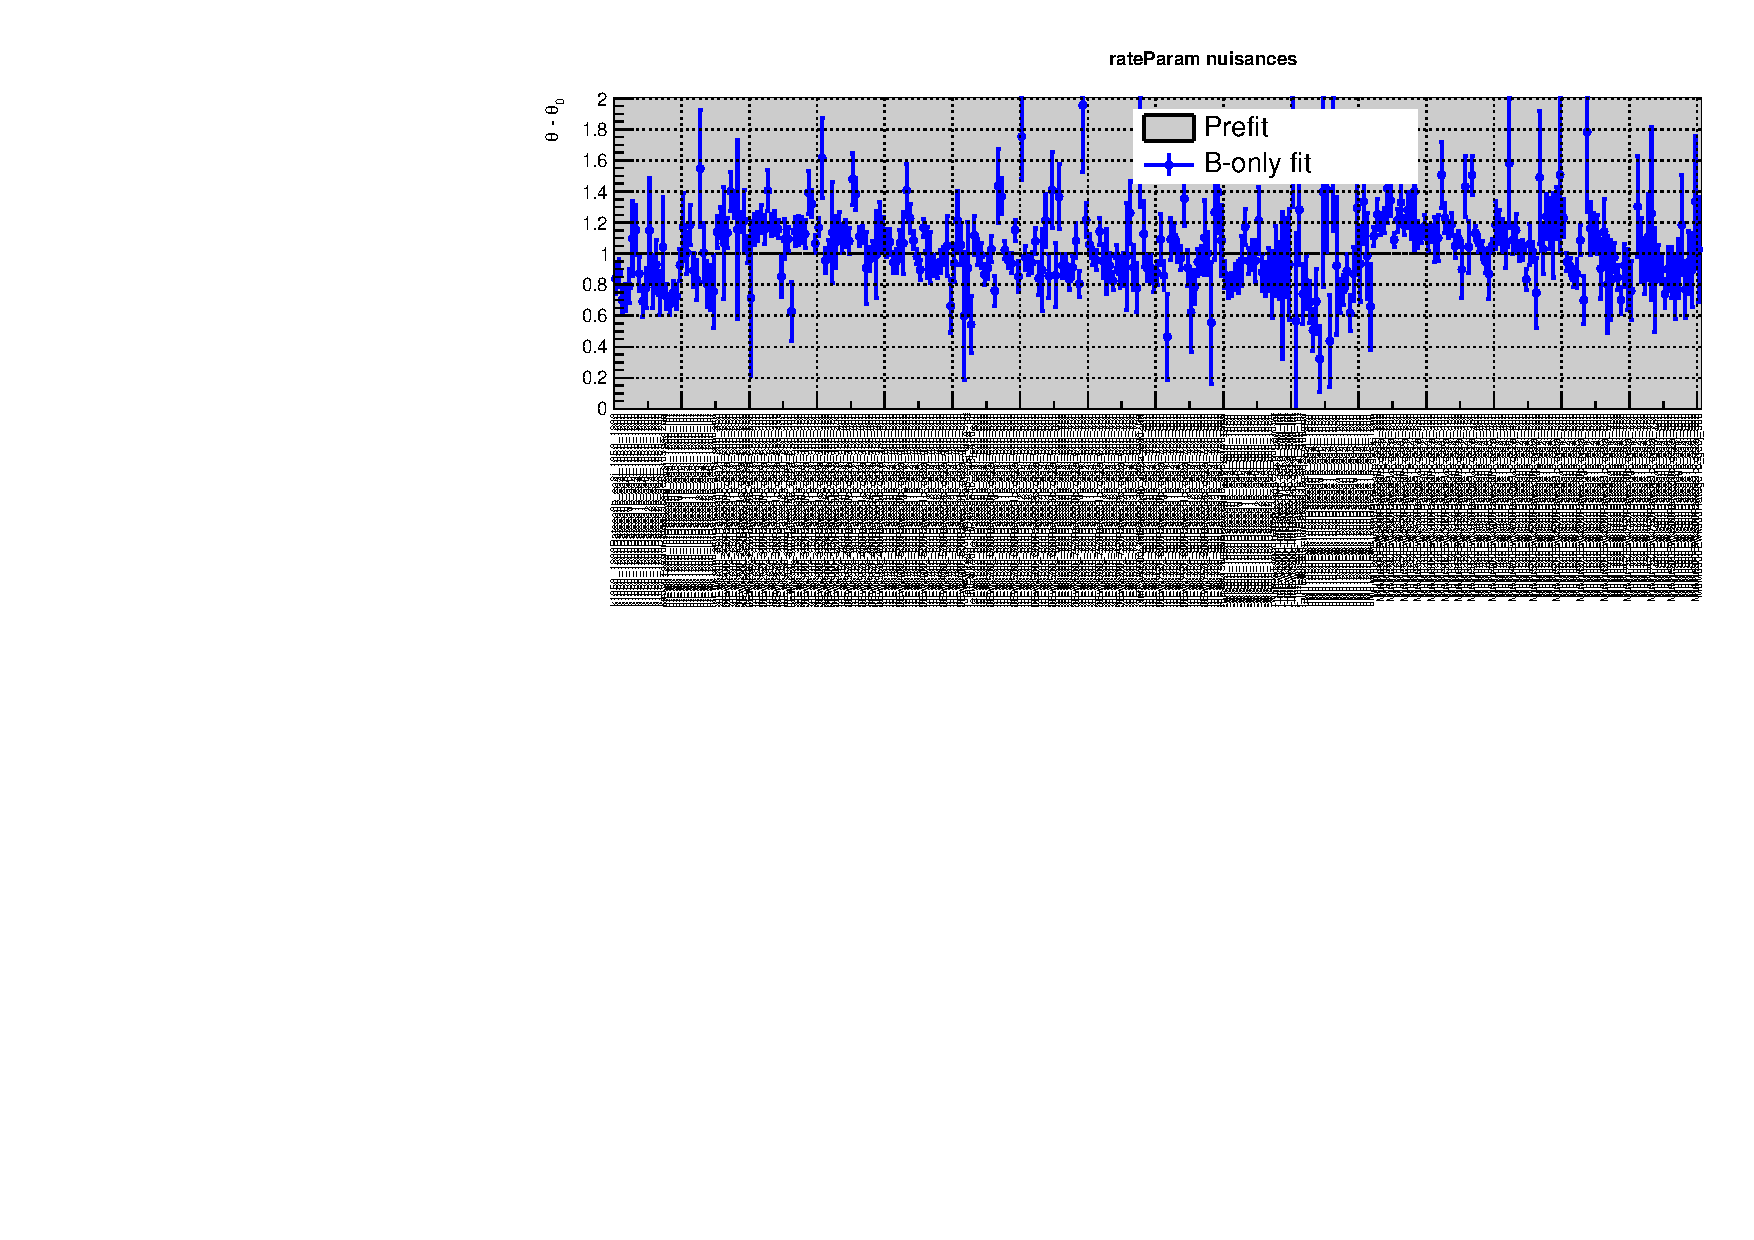
\includegraphics[width=1.\linewidth]{figures/results/36invfb/prefit/nuis/Rates_nuisances}
%\end{figure}
%
%\begin{figure}[h!]
%  \centering
%  \caption{Correlated sources of uncertainty}
%  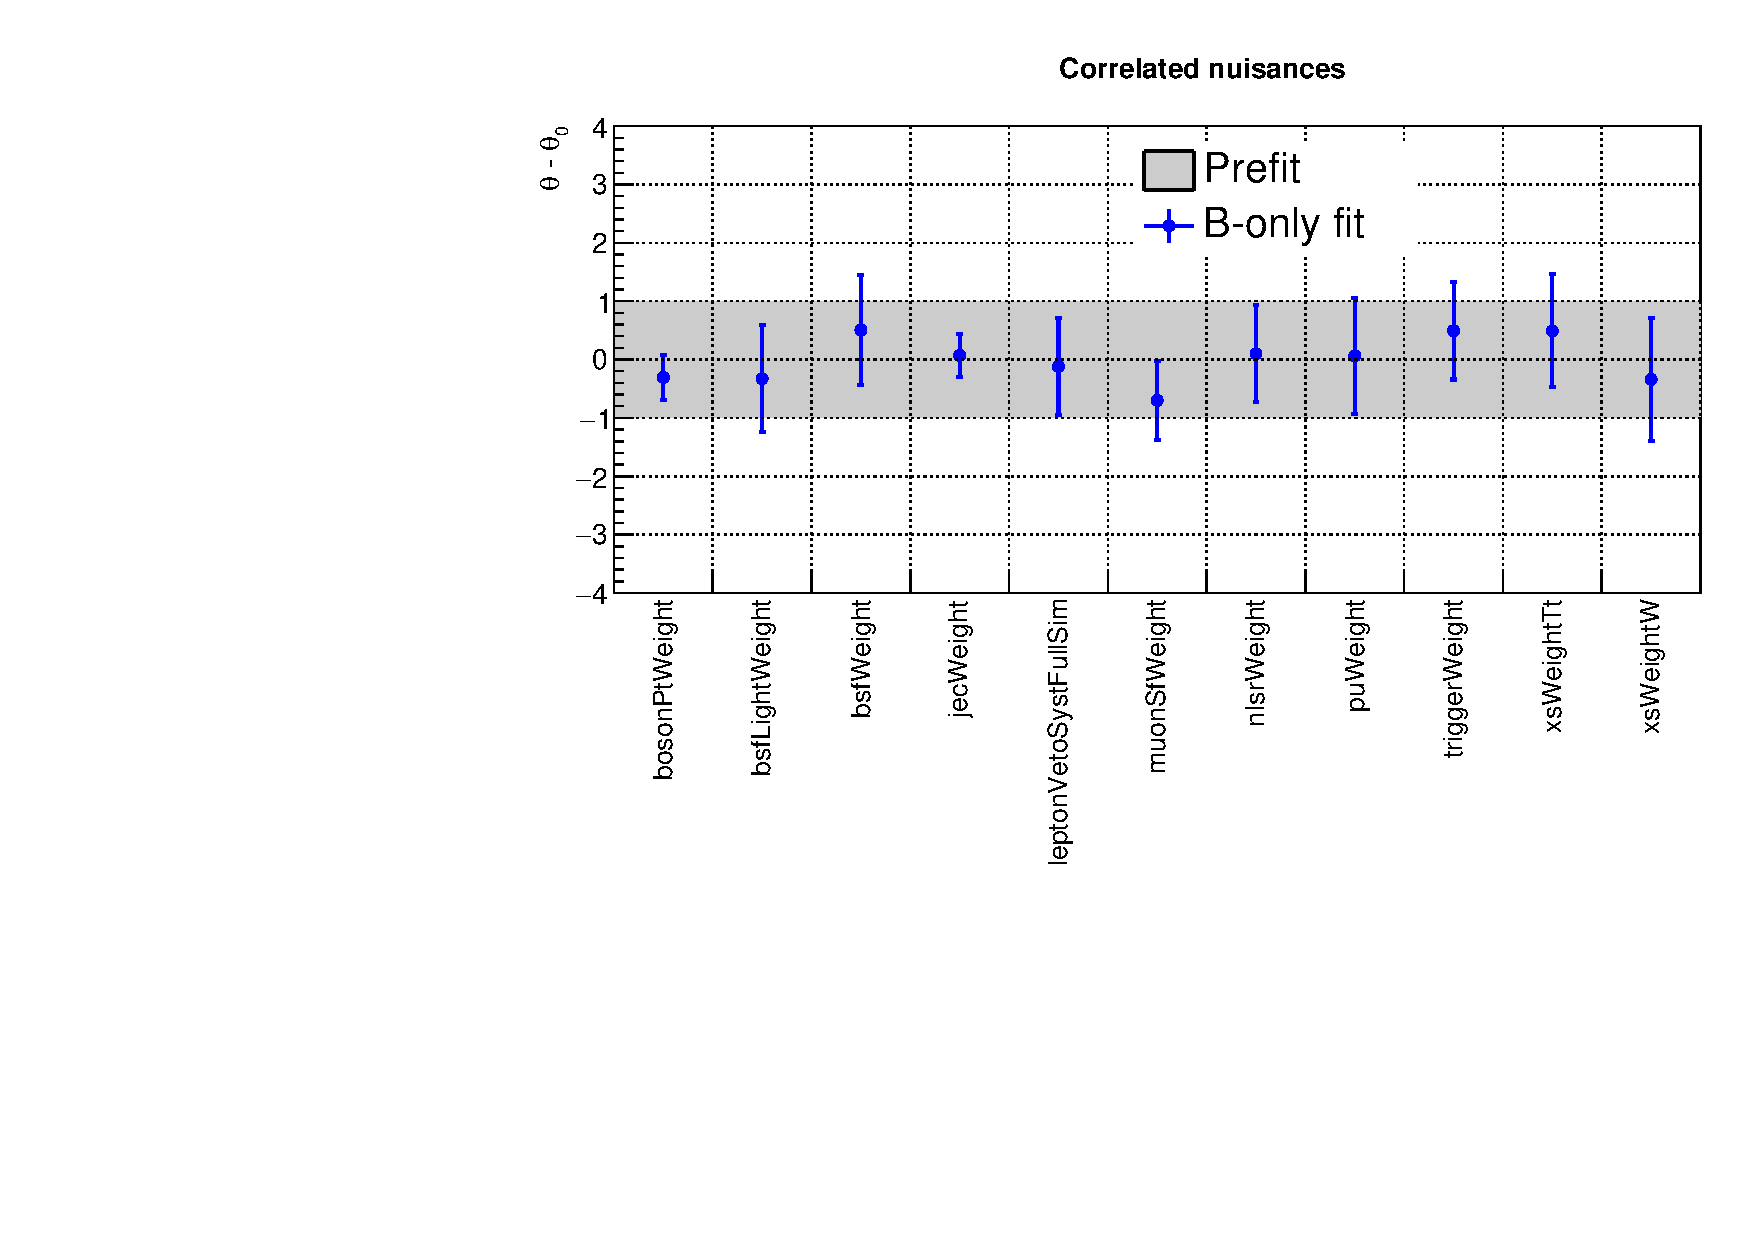
\includegraphics[width=1.\linewidth]{figures/results/36invfb/prefit/nuis/Correlated_nuisances}
%\end{figure}

\clearpage
\subsection{Post-fit nuisance parameters}
\label{app:nuispost}

\begin{figure}[h!]
  \centering
  \caption{Rate parameters}
  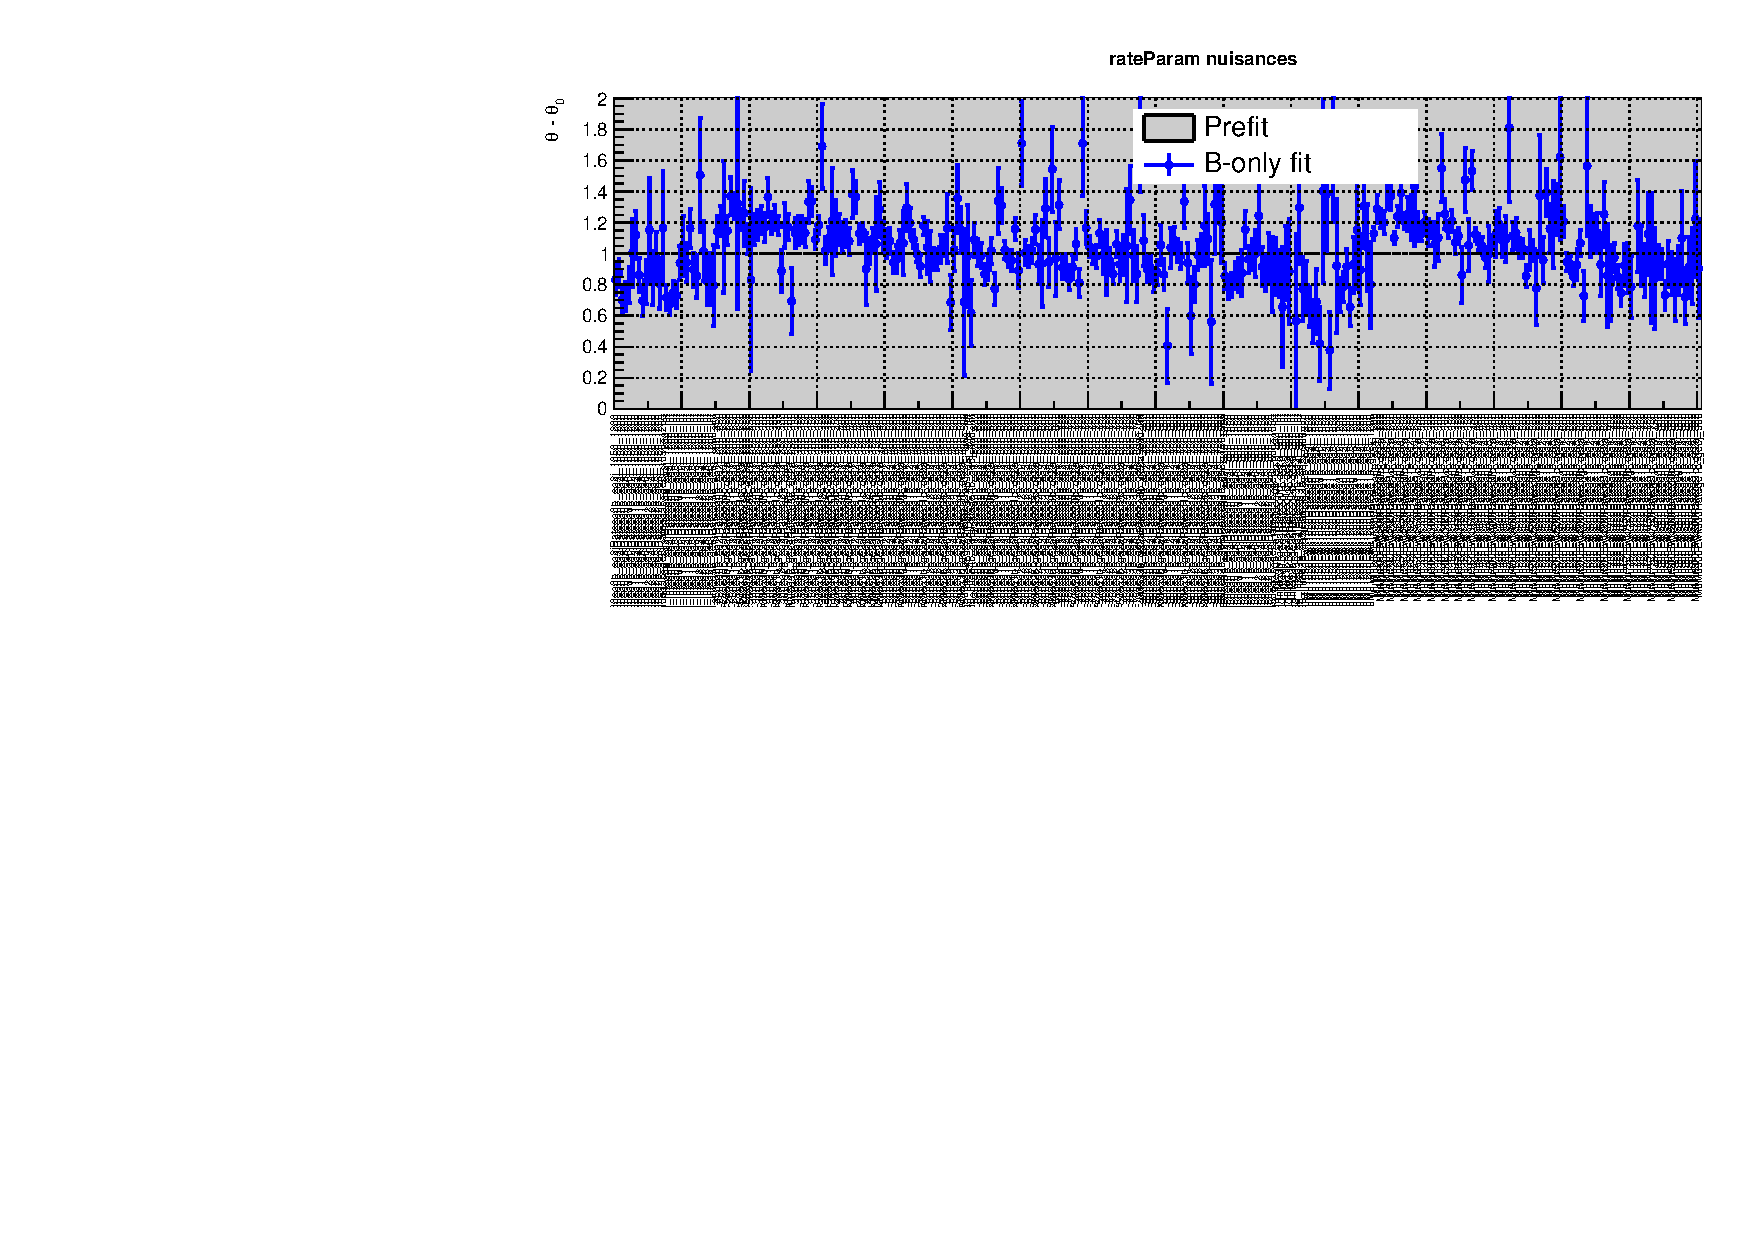
\includegraphics[width=1.\linewidth]{figures/results/36invfb_preapproval/postfit/nuis/Rates_nuisances}
\end{figure}

\begin{figure}[h!]
  \centering
  \caption{Correlated sources of uncertainty}
  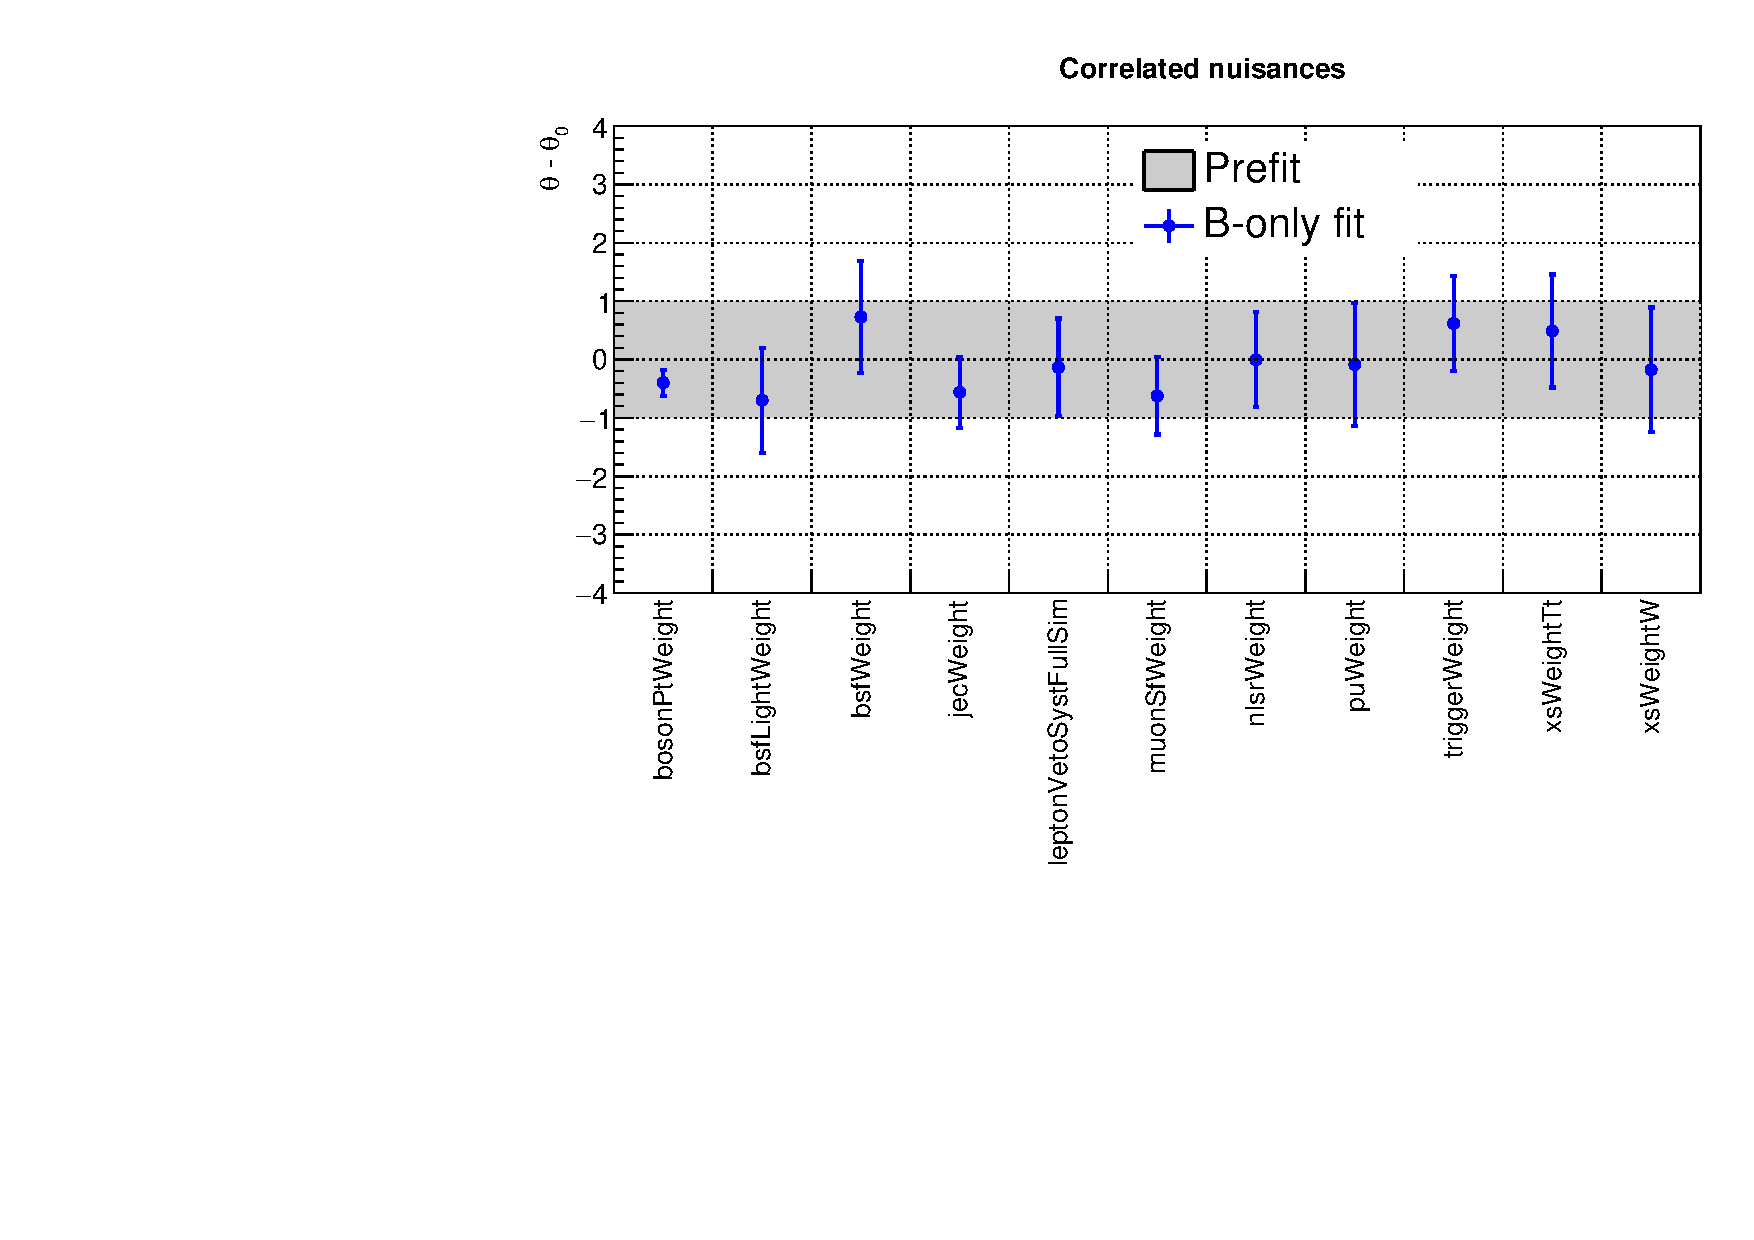
\includegraphics[width=1.\linewidth]{figures/results/36invfb_preapproval/postfit/nuis/Correlated_nuisances}
\end{figure}

\clearpage
\begin{figure}[h!]
  \centering
  \caption{``MC stat.'' uncertainties for lost lepton background.}
  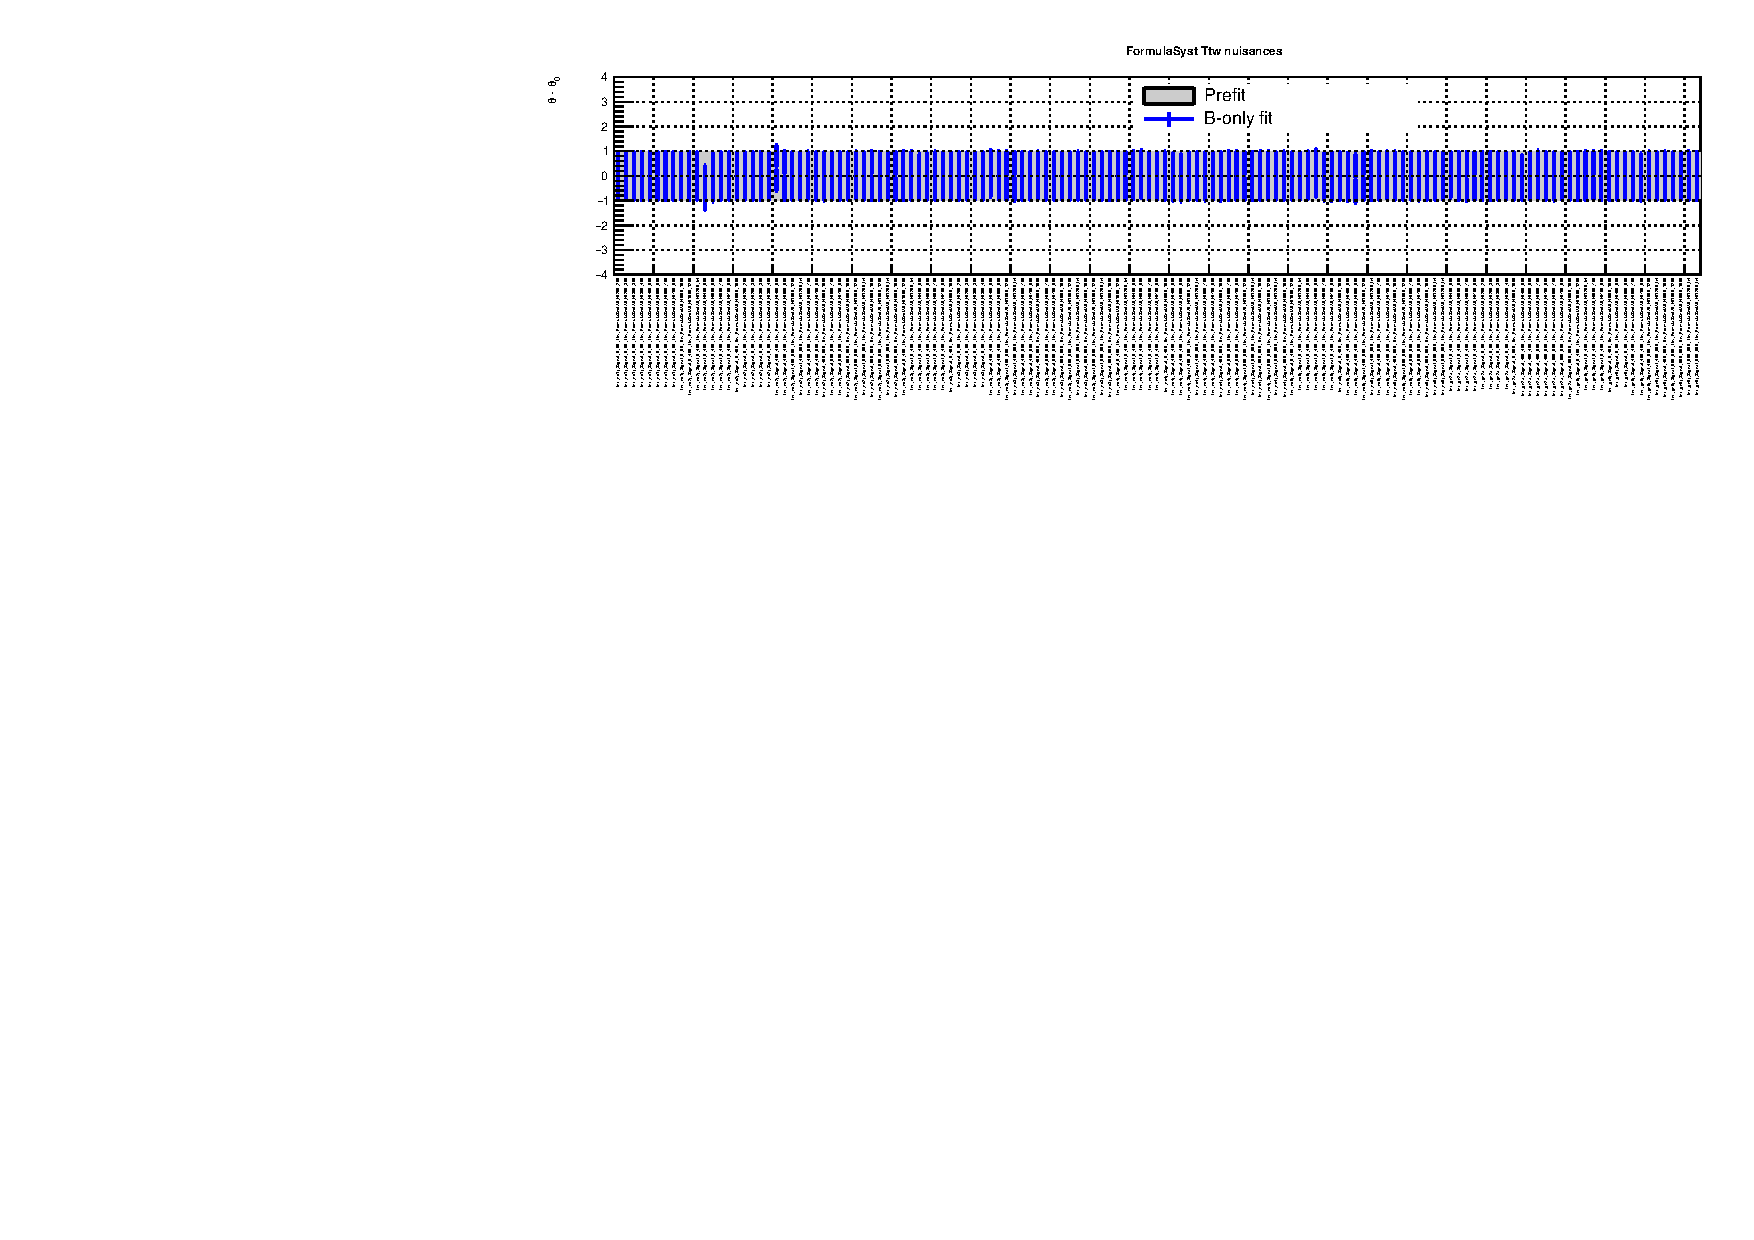
\includegraphics[width=1.\linewidth]{figures/results/36invfb_preapproval/postfit/nuis/FormulaSystTtw_nuisances}
\end{figure}

\begin{figure}[h!]
  \centering
  \caption{``MC stat.'' uncertainties for \znunuj background.}
  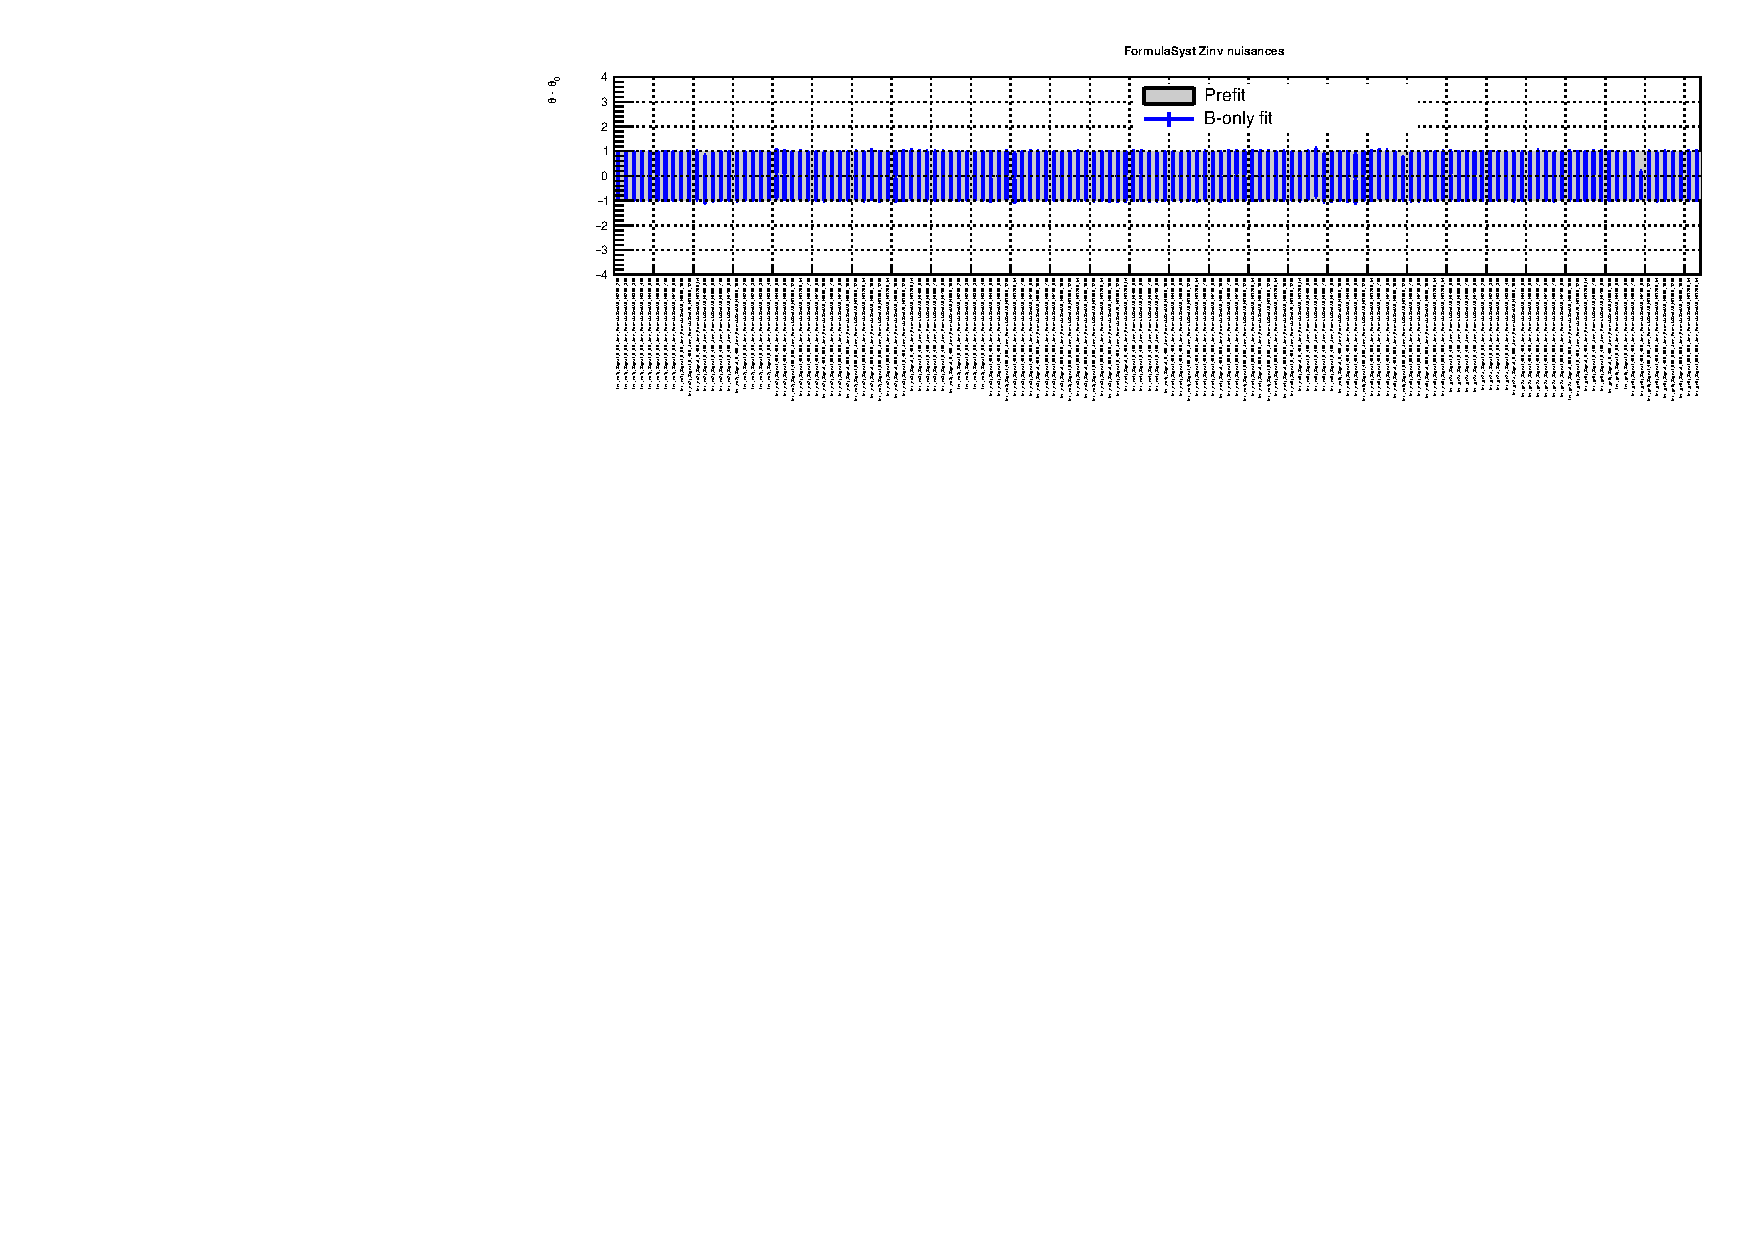
\includegraphics[width=1.\linewidth]{figures/results/36invfb_preapproval/postfit/nuis/FormulaSystZinv_nuisances}
\end{figure}

\clearpage
\begin{figure}[h!]
  \centering
  \caption{Systematic uncertainties in QCD background estimate}
  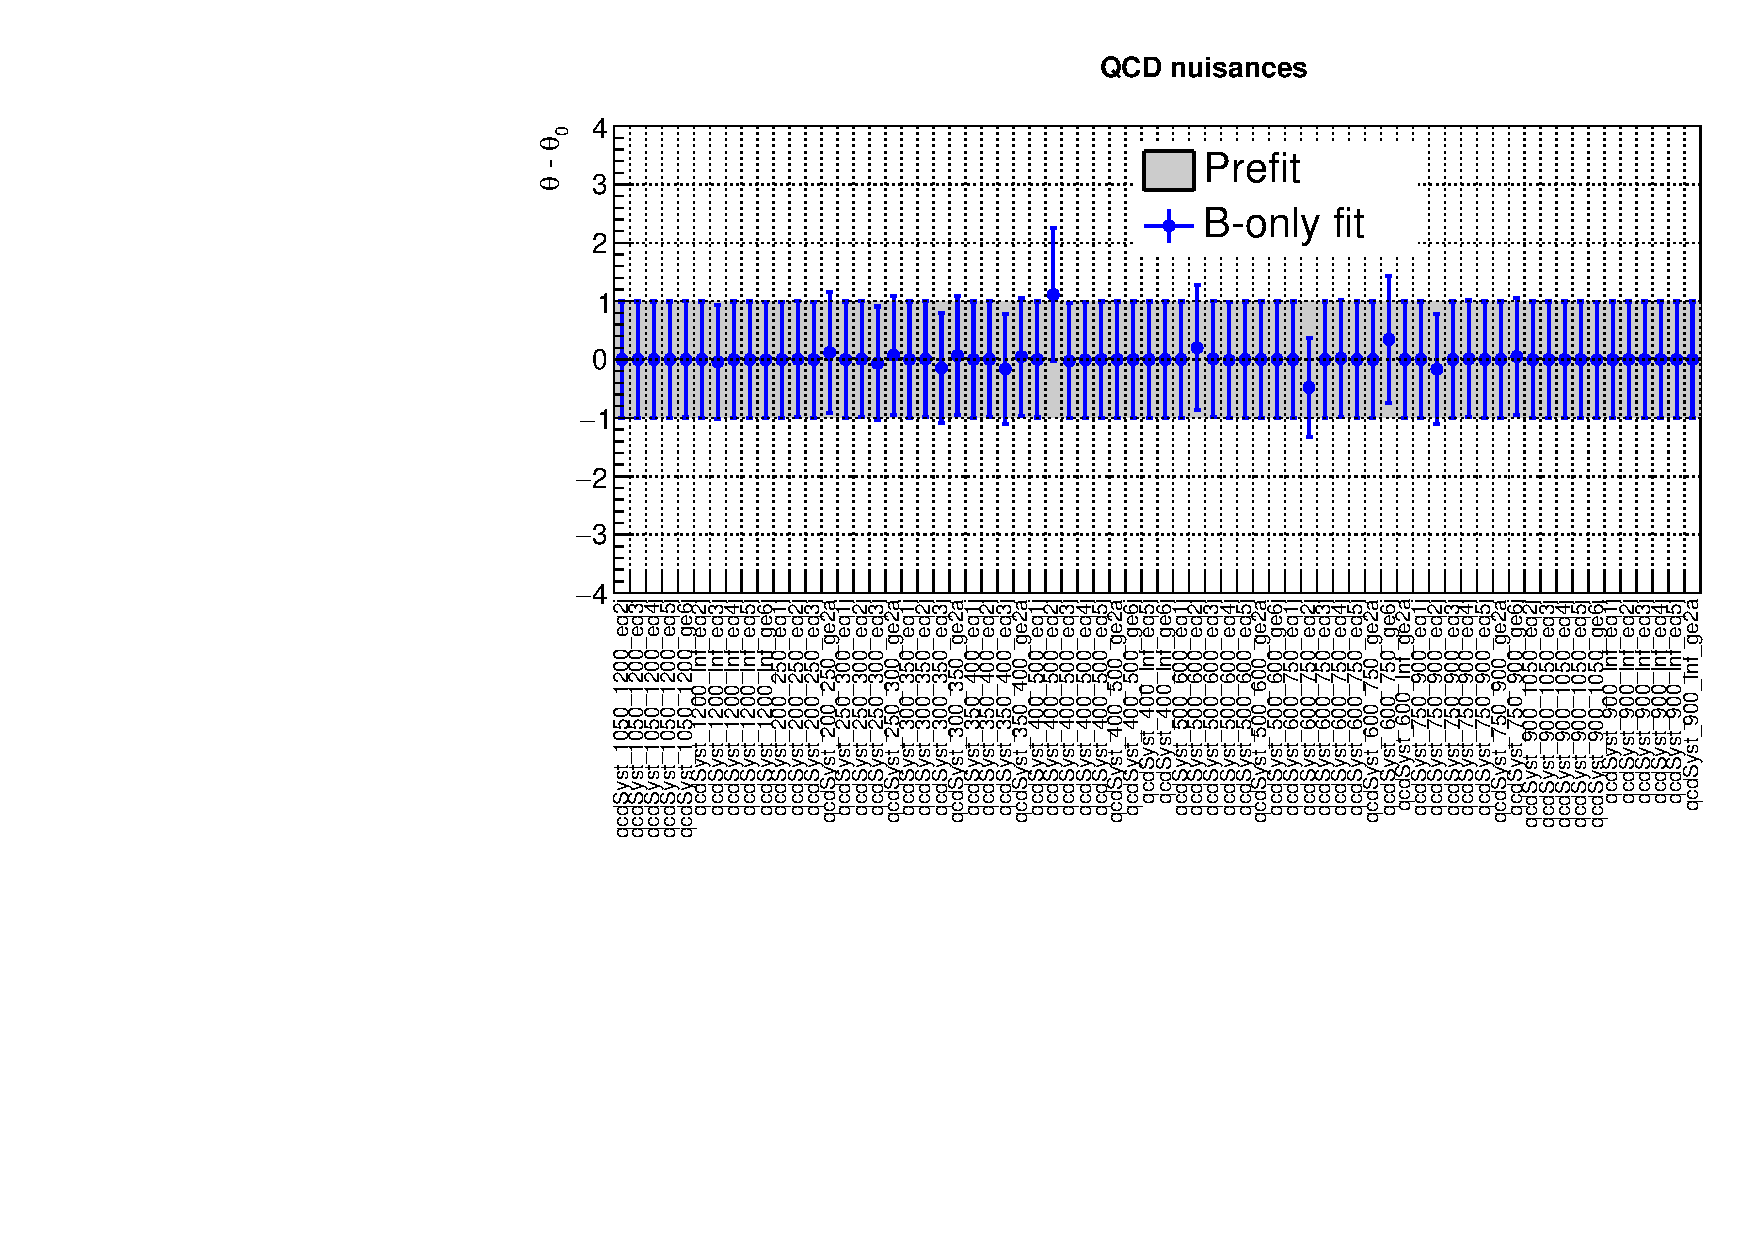
\includegraphics[width=1.\linewidth]{figures/results/36invfb_preapproval/postfit/nuis/qcd_nuisances}
\end{figure}

\clearpage
\begin{figure}[h!]
  \centering
  \caption{Systematic uncertainties per \scalht category in \mht modelling for lost lepton background}
  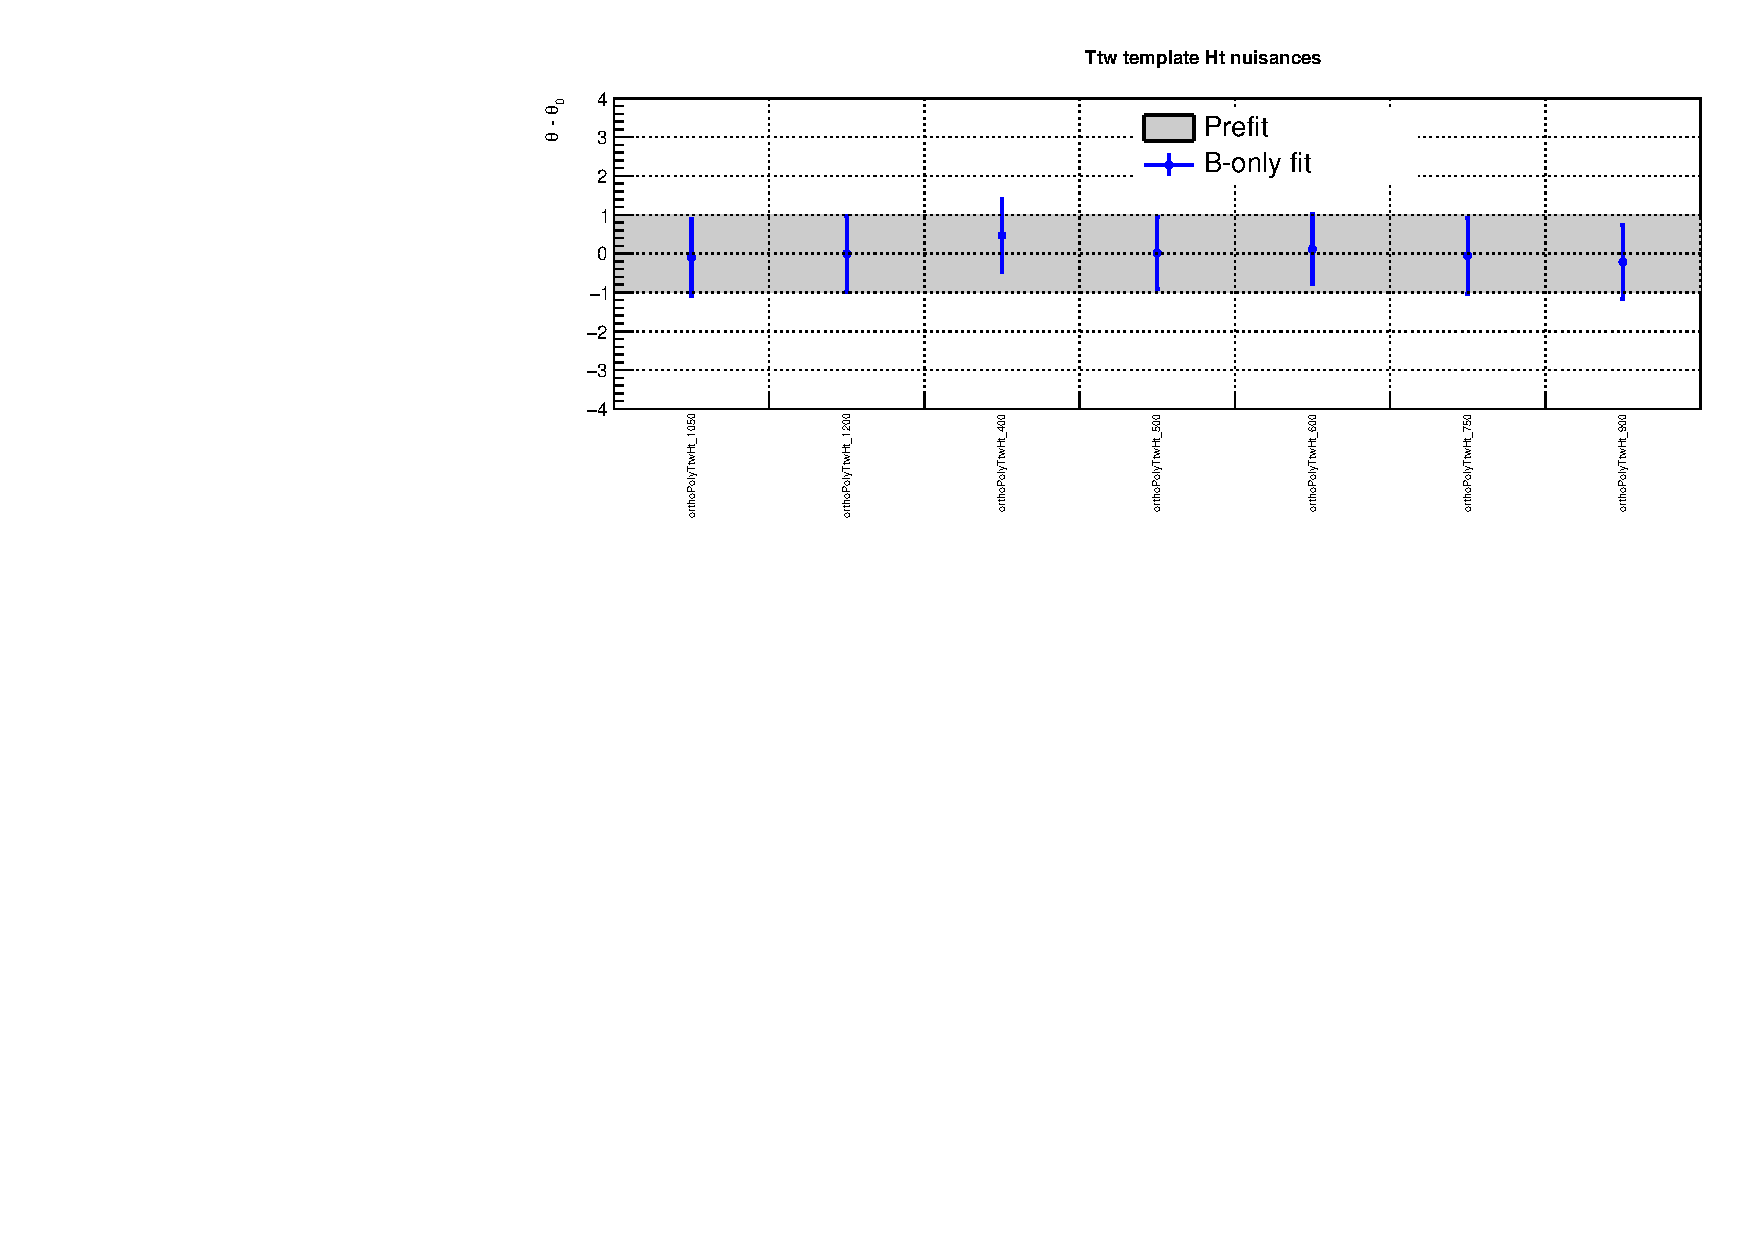
\includegraphics[width=1.\linewidth]{figures/results/36invfb_preapproval/postfit/nuis/TemplateTtw_ht_nuisances}
\end{figure}

\begin{figure}[h!]
  \centering
  \caption{Systematic uncertainties per \njet category in \mht modelling for lost lepton background}
  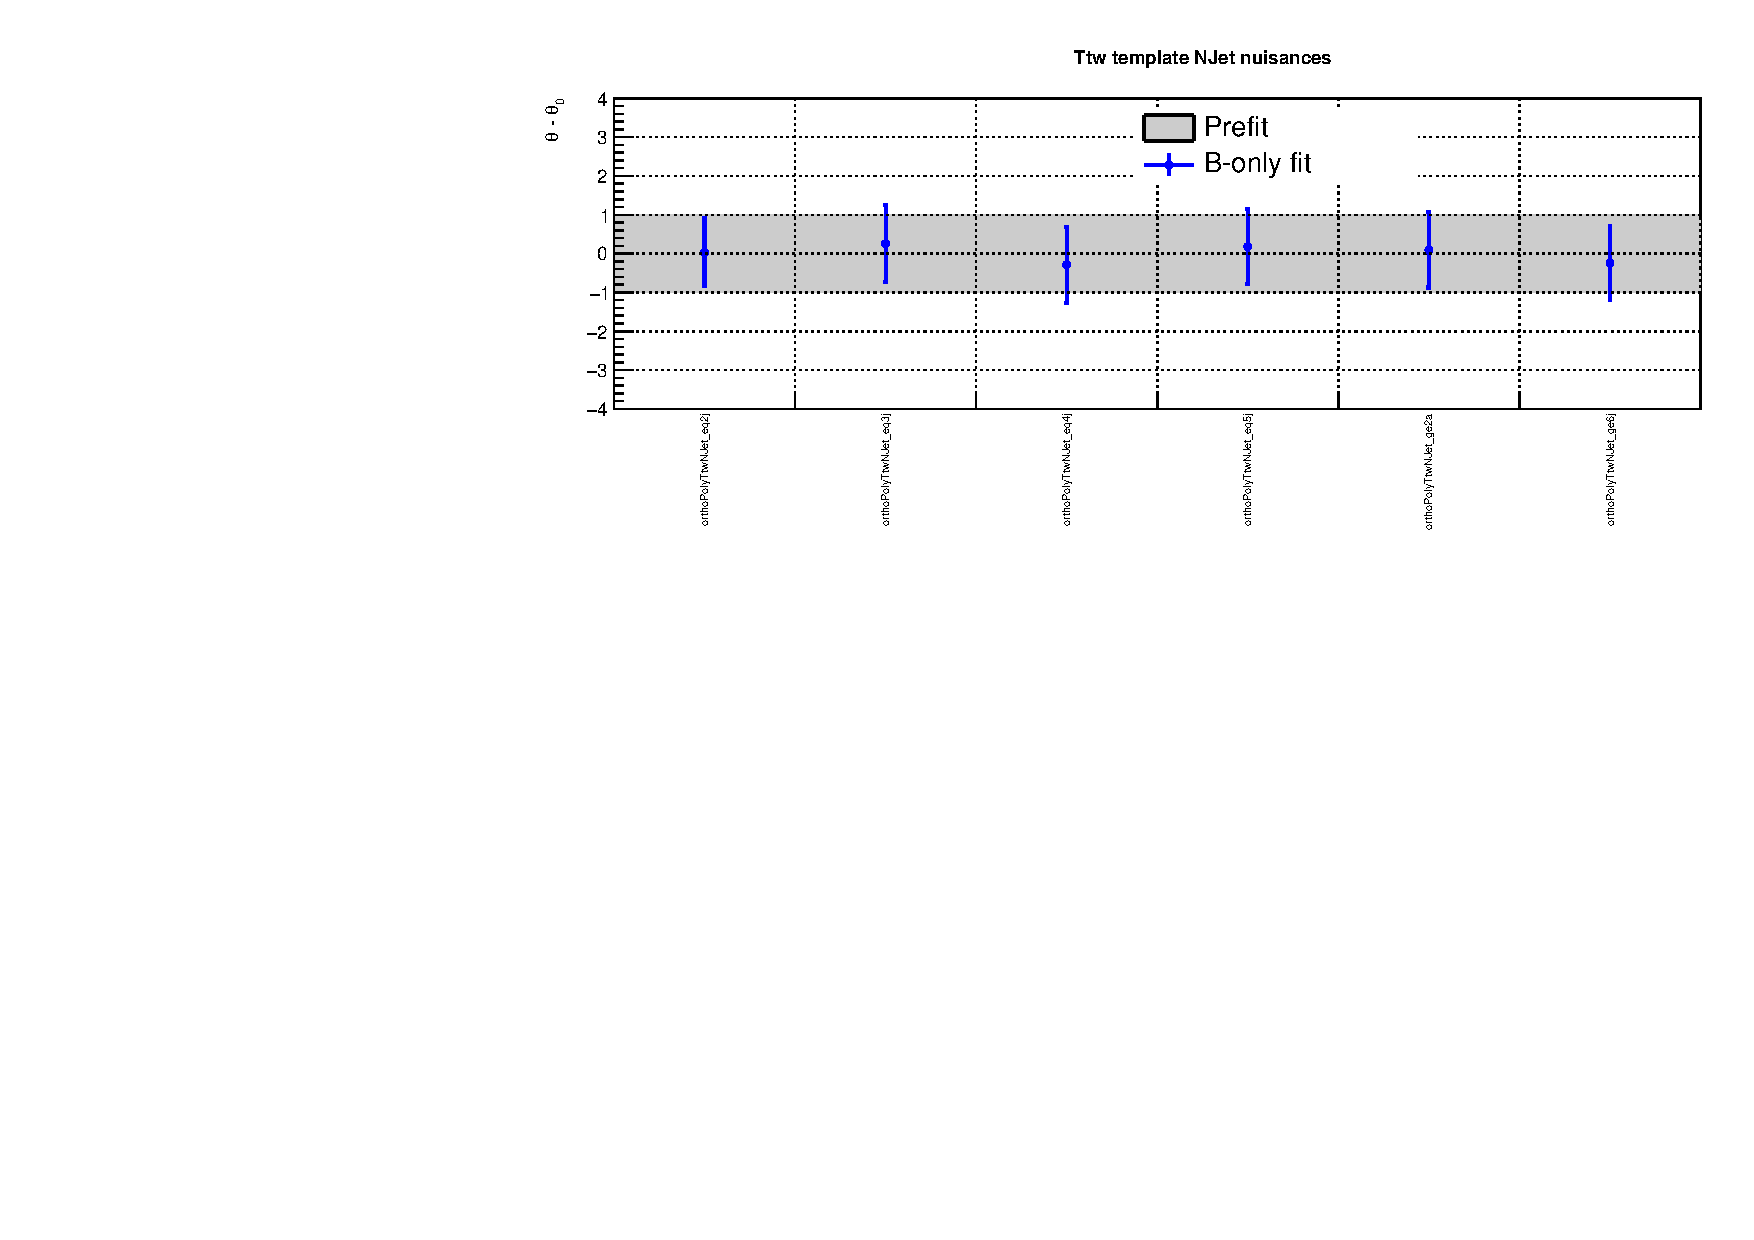
\includegraphics[width=1.\linewidth]{figures/results/36invfb_preapproval/postfit/nuis/TemplateTtw_njet_nuisances}
\end{figure}

\clearpage
\begin{figure}[h!]
  \centering
  \caption{Systematic uncertainties per \scalht category in \mht modelling for \znunuj background}
  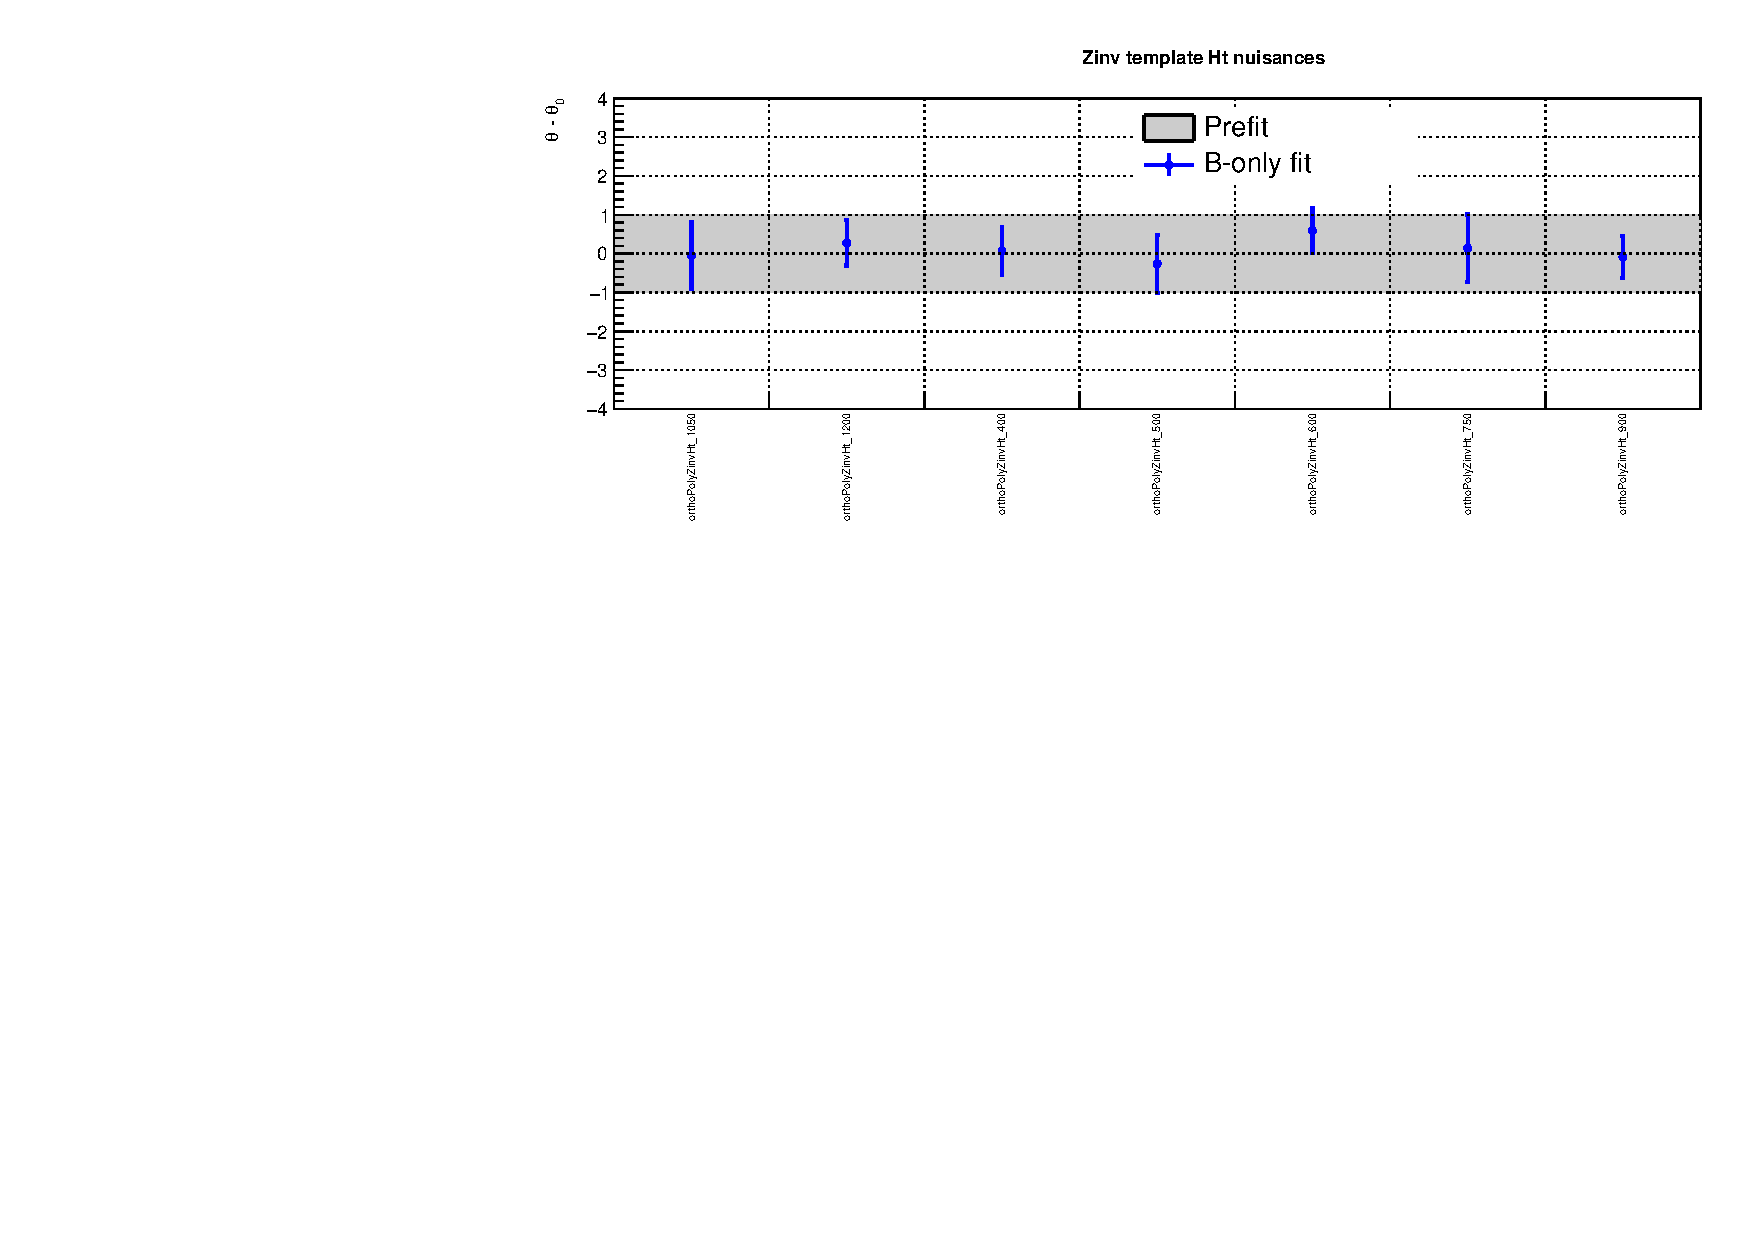
\includegraphics[width=1.\linewidth]{figures/results/36invfb_preapproval/postfit/nuis/TemplateZinv_ht_nuisances}
\end{figure}

\begin{figure}[h!]
  \centering
  \caption{Systematic uncertainties per \njet category in \mht modelling for \znunuj background}
  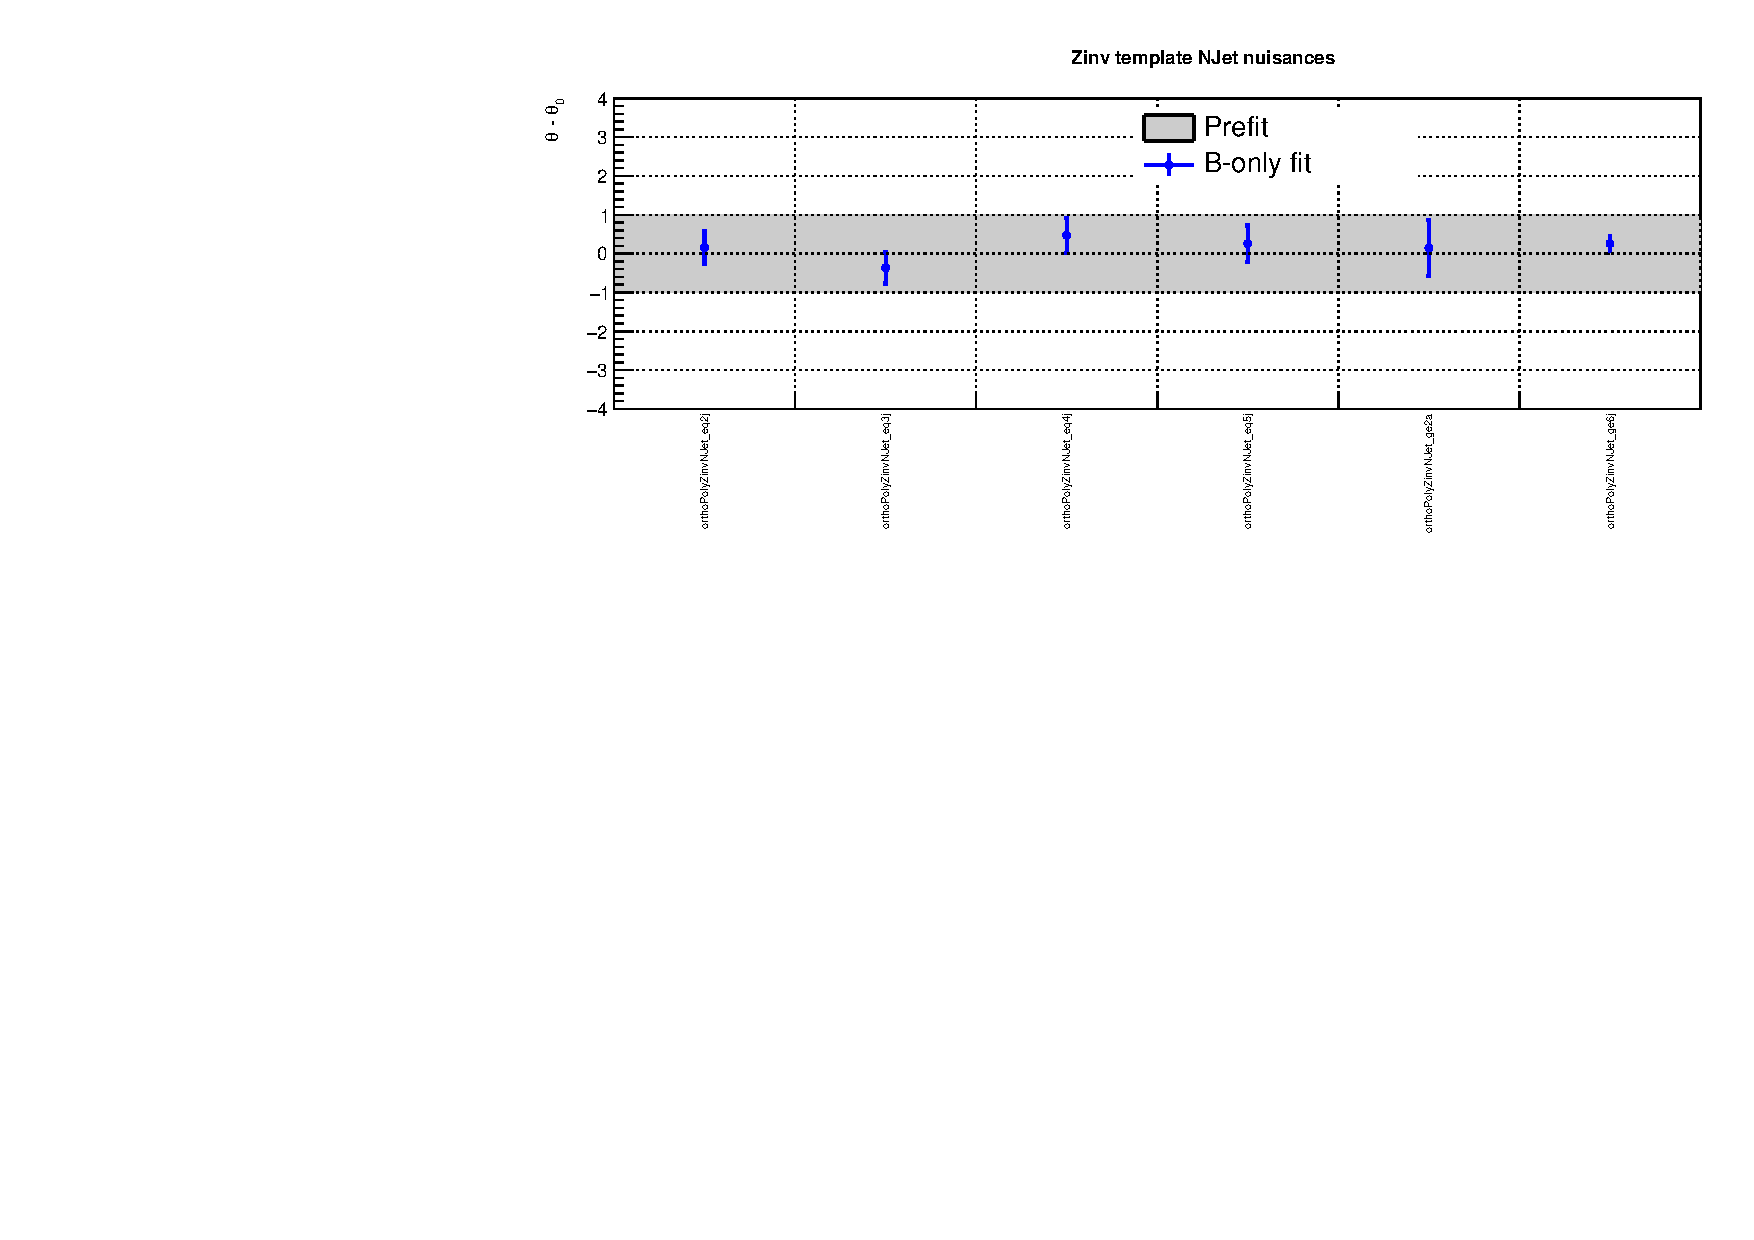
\includegraphics[width=1.\linewidth]{figures/results/36invfb_preapproval/postfit/nuis/TemplateZinv_njet_nuisances}
\end{figure}

\clearpage
\begin{figure}[h!]
  \centering
  \caption{Systematic uncertainties in \alphat modelling}
  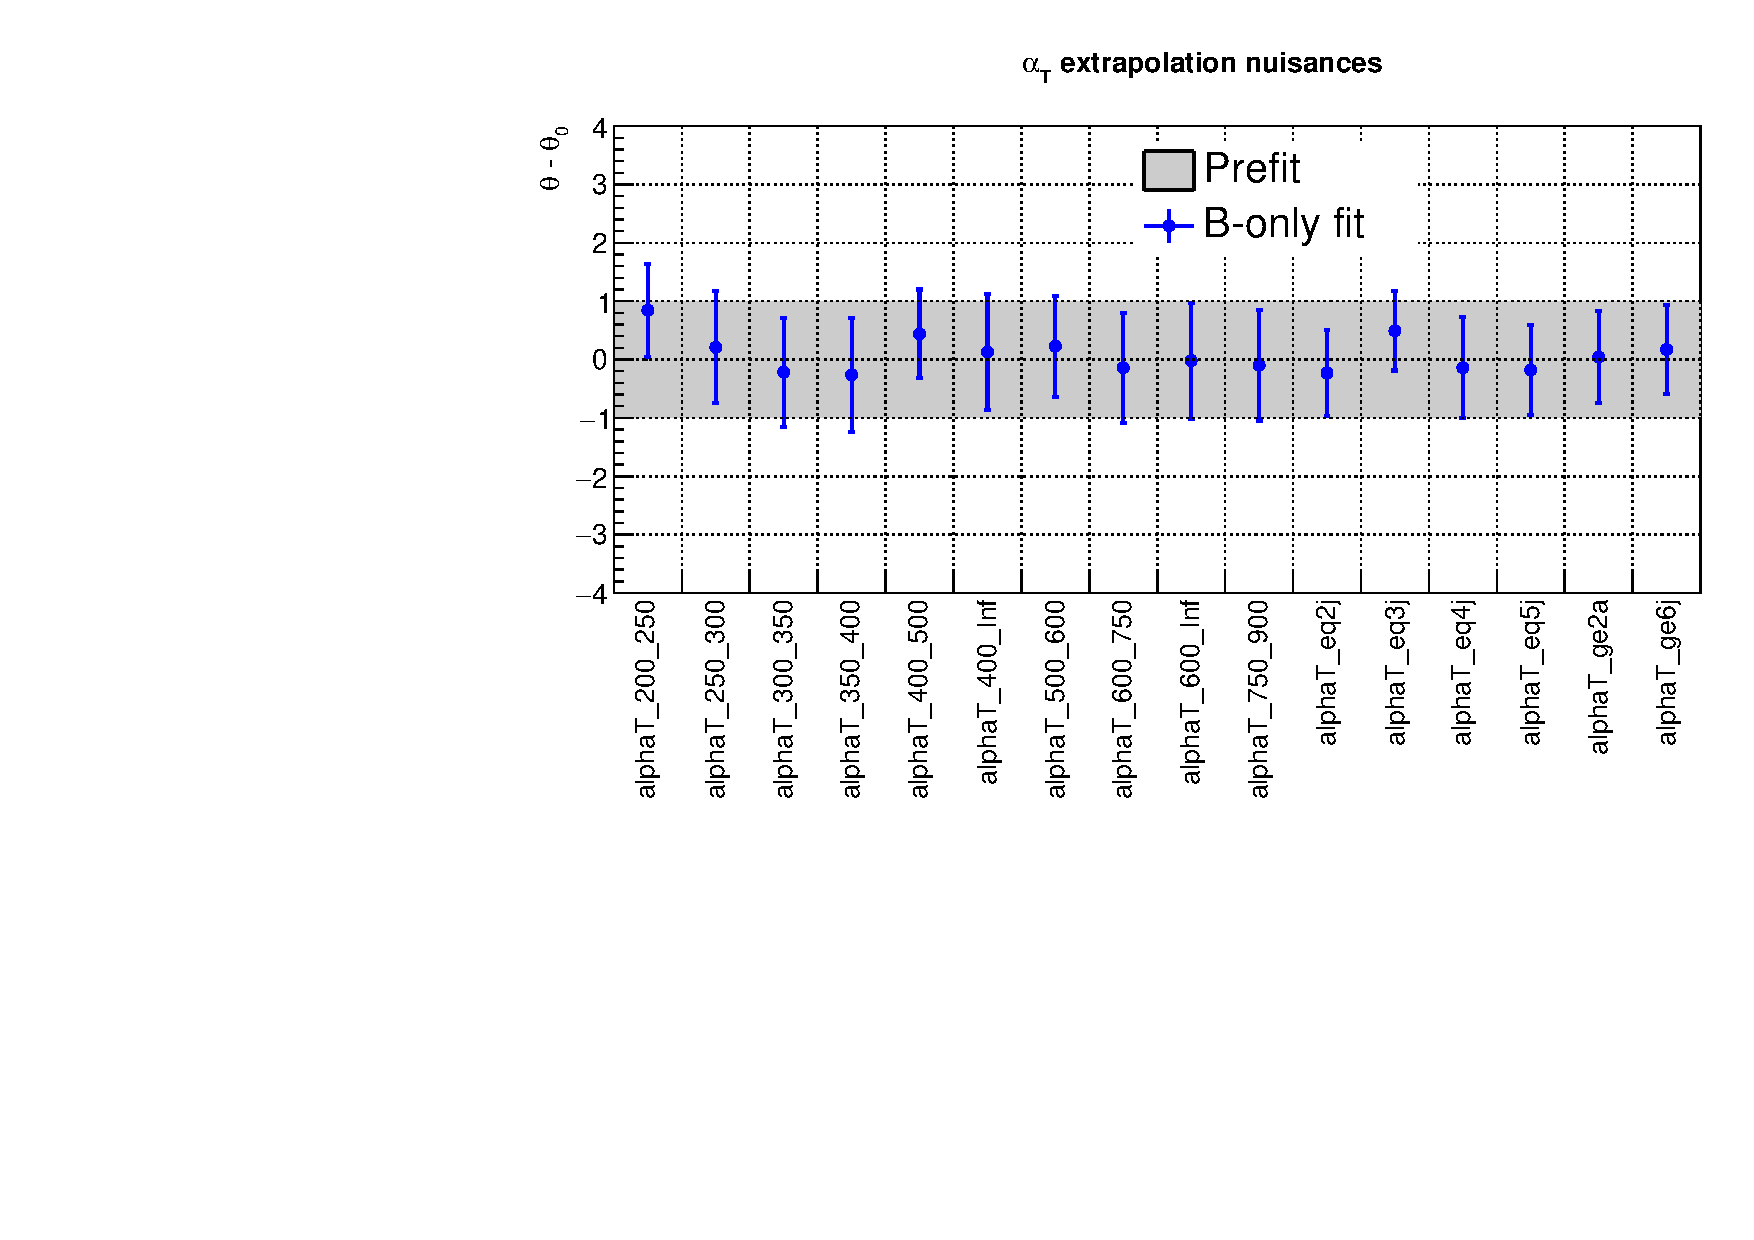
\includegraphics[width=0.8\linewidth]{figures/results/36invfb_preapproval/postfit/nuis/AlphaT_nuisances}
\end{figure}

\begin{figure}[h!]
  \centering
  \caption{Systematic uncertainties in \bdphi modelling}
  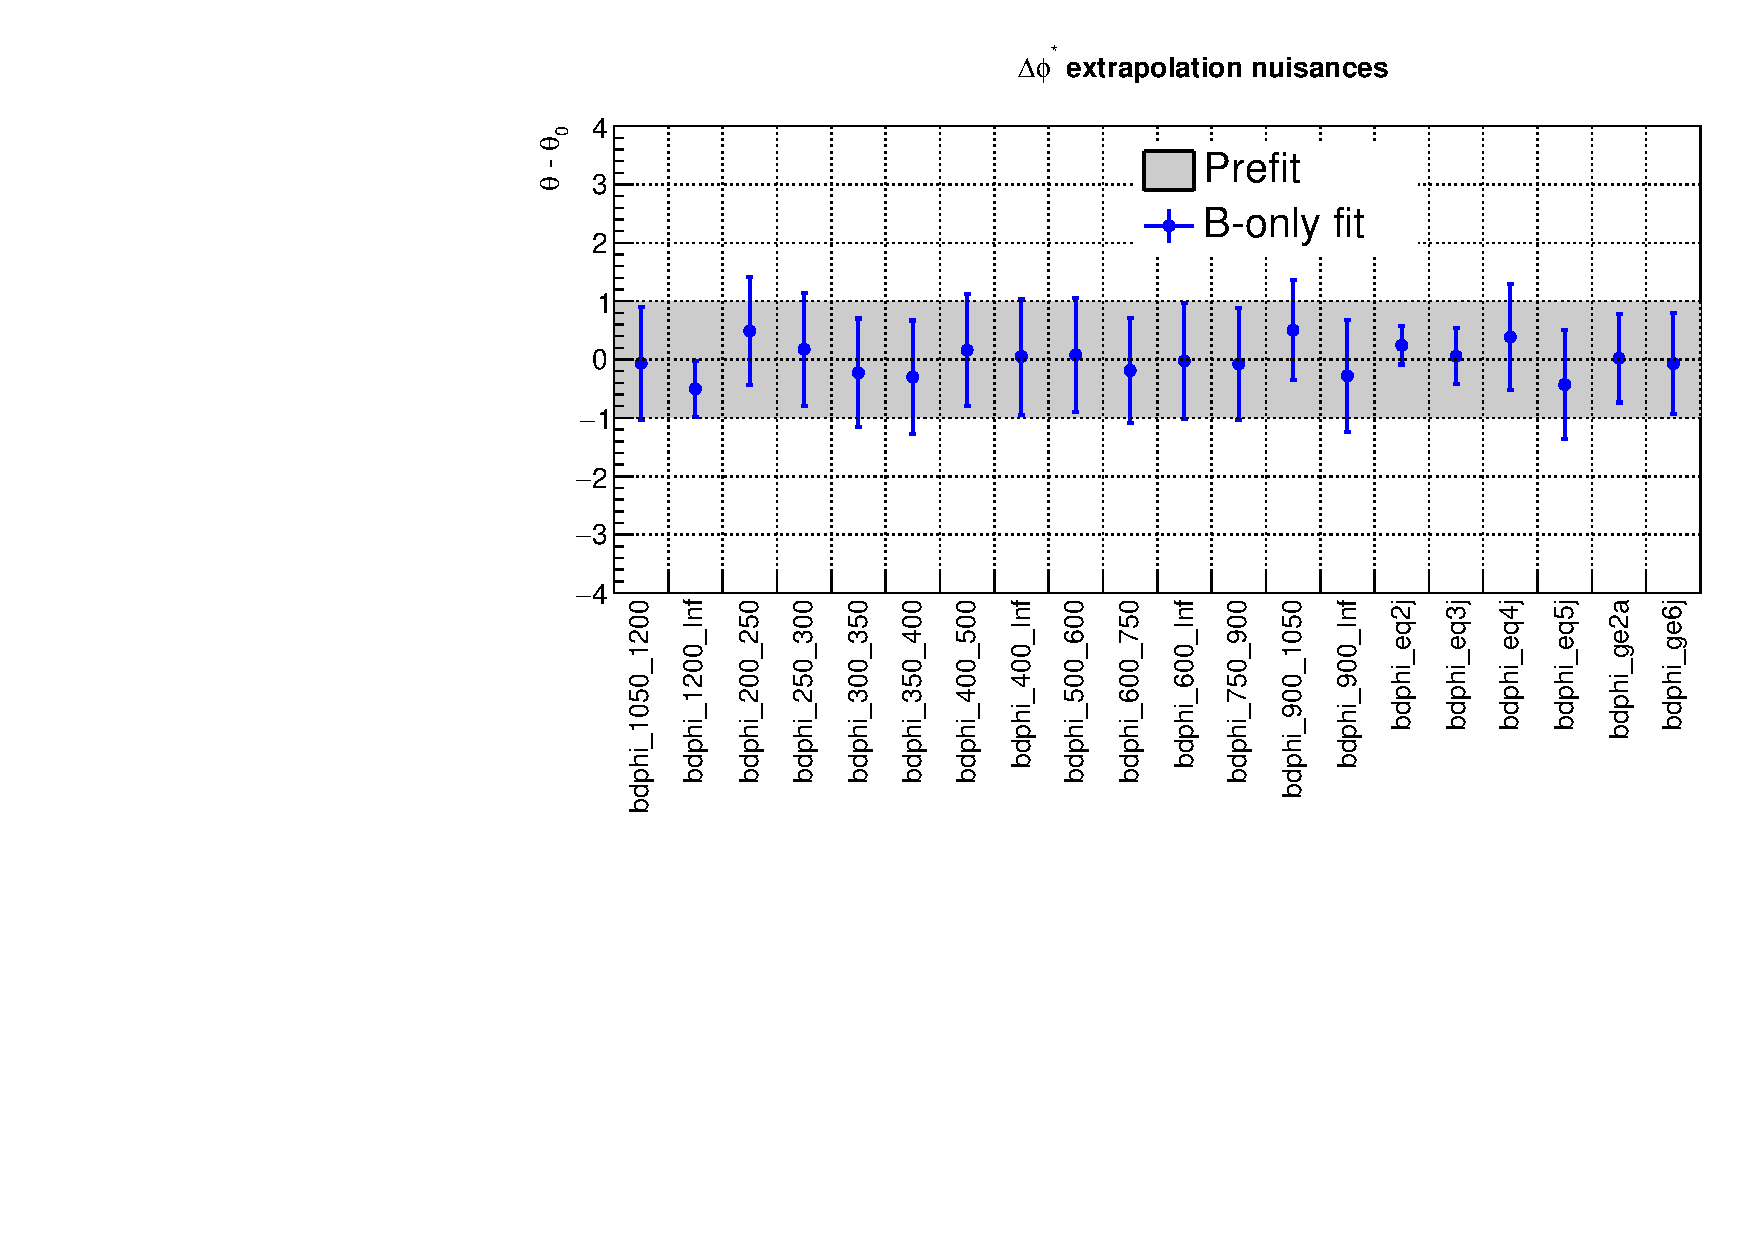
\includegraphics[width=0.8\linewidth]{figures/results/36invfb_preapproval/postfit/nuis/bDPhi_nuisances}
\end{figure}

\clearpage
\begin{figure}[h!]
  \centering
  \caption{Systematic uncertainties in single isolated track veto modelling}
  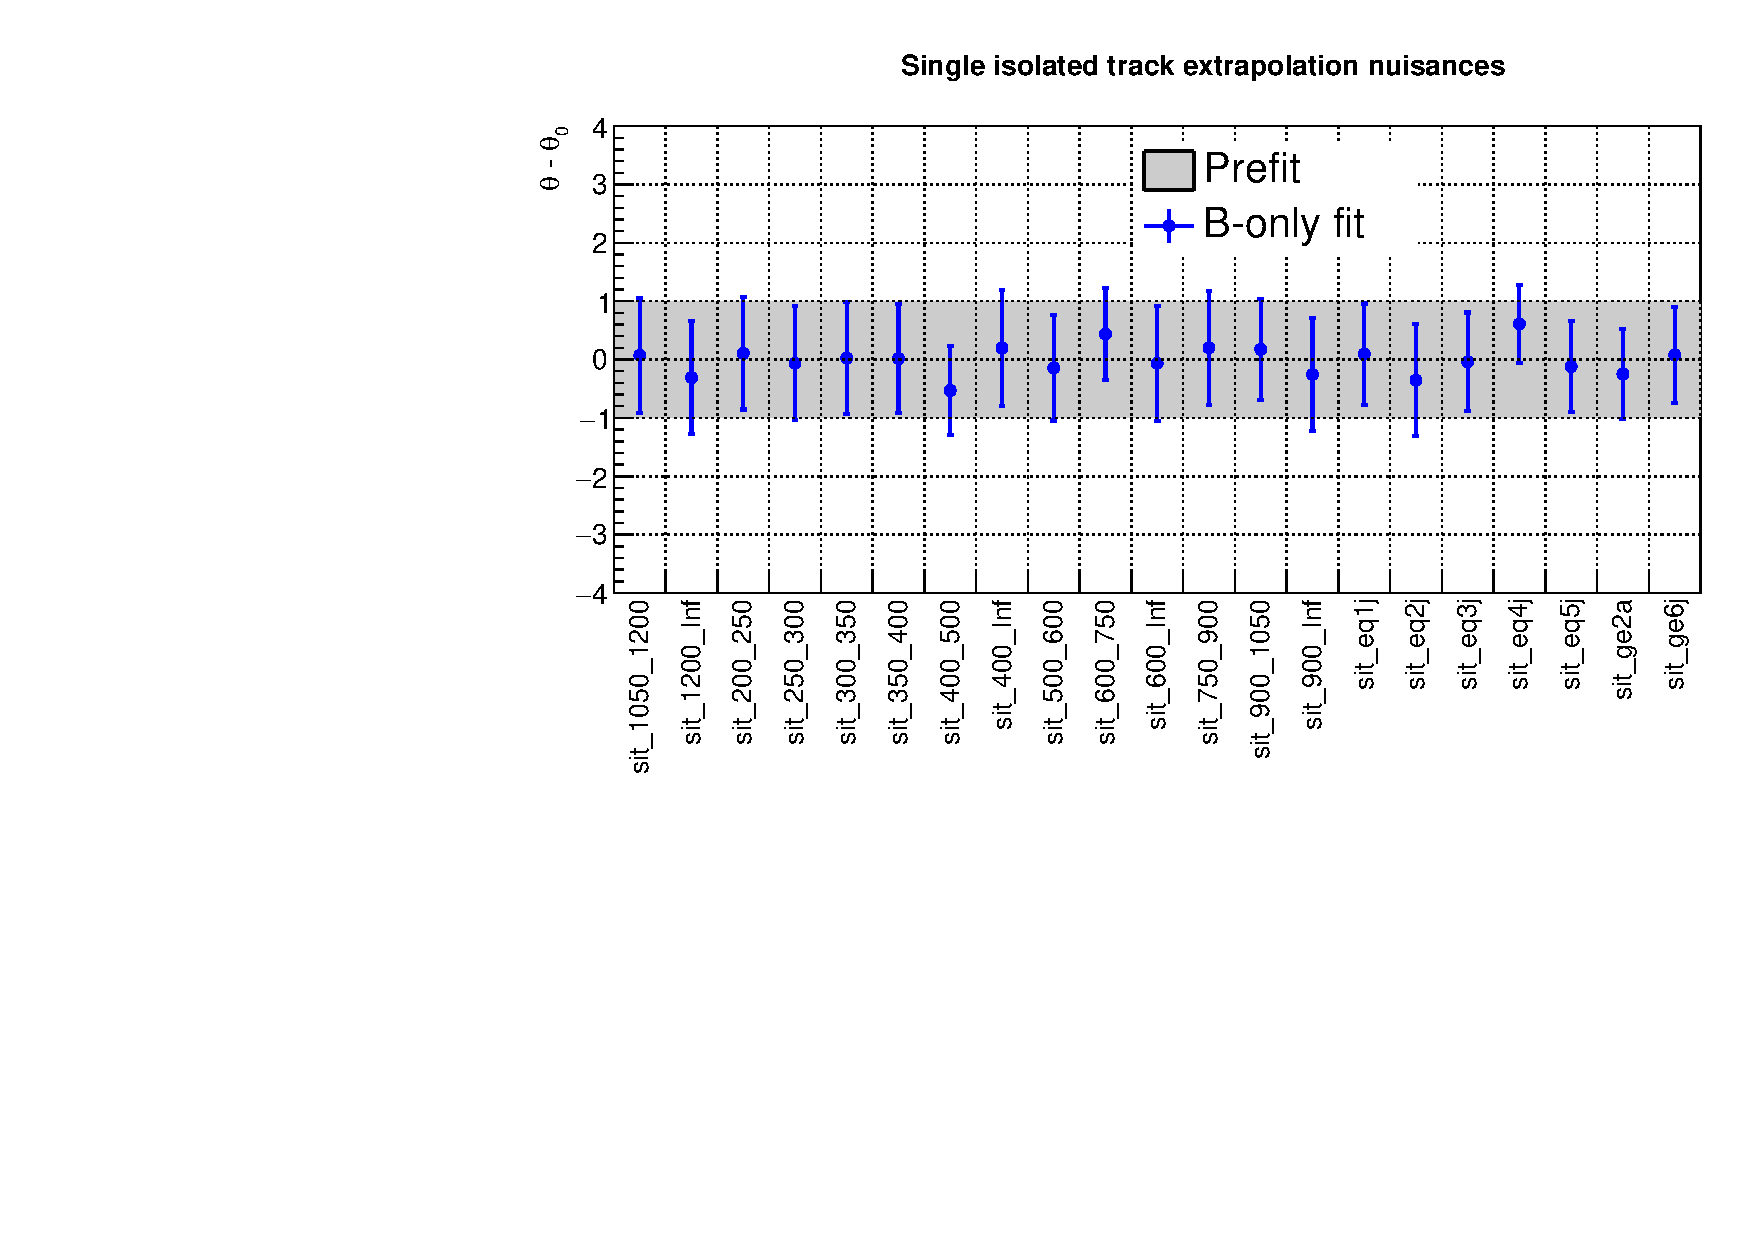
\includegraphics[width=0.8\linewidth]{figures/results/36invfb_preapproval/postfit/nuis/SIT_nuisances}
\end{figure}

\clearpage
\begin{figure}[h!]
  \centering
  \caption{Systematic uncertainties in W polarisation modelling}
  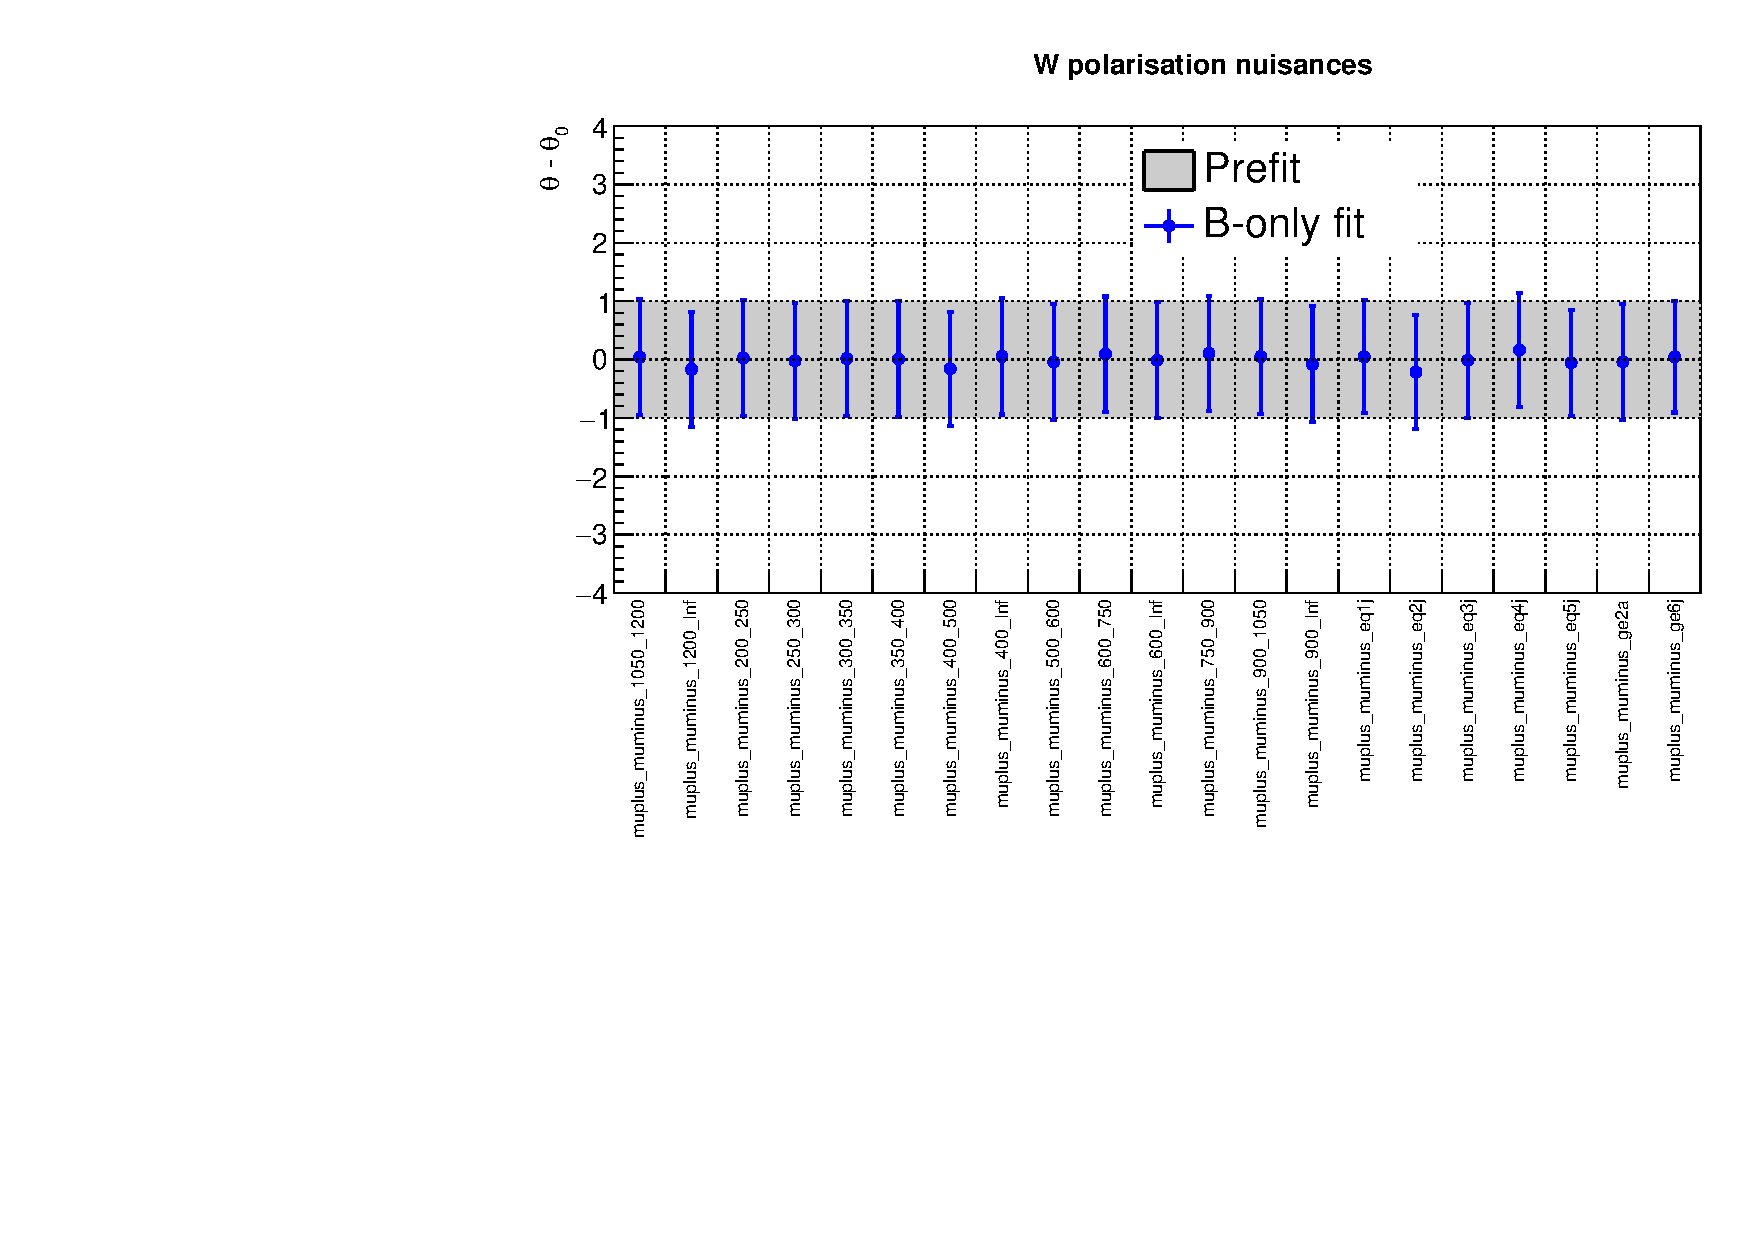
\includegraphics[width=0.8\linewidth]{figures/results/36invfb_preapproval/postfit/nuis/WPol_nuisances}
\end{figure}
